\chapter{安全:可扩展身份认证协议、IP 安全协议、传输层\\ 
安全、DNS 安全、域名密钥识别邮件}
\section{引言}
本章将会介绍与 TCP/IP一同使用的安全方案。安全是一个内容广泛又十分有趣的话题,
其涵盖的内容远远超出了本书所涉及的范围。因此,本章将着重介绍互联网上的安全威胁,
并详细讨论抵御这些威胁的安全机制。这些安全机制适用于各种协议,比如IP、TCP 以及重
要的电子邮件与 DNS应用协议。

虽然下述分类并不正式,但安全威胁一般可以根据执行目标的不同分为三类攻击:试图
颠覆已有过程来运行其他不应该执行的代码;试图获得用户权限来运行恶意程序;采用未经
授权的方法使用兼容的网络协议。本书的其他章节已经介绍过一些上述形式的攻击。例如,
互联网最早的蠕虫(自我繁殖软件)之一就是利用了缓冲区溢出的问题重写服务器进程的内
存。客户端程序能够将蠕虫软件注入服务器中,从而使服务器最终运行注人的代码。注人的
代码还会重复上述动作,从而实现自身的繁殖。因此,这种代码会比简单的自我繁殖带来更
多的危害。

各种类型的攻击与技术能够结合起来。随着互联网上信息价值的不断提升,复杂的软件
与安全分析工具也在不断发展。一些文章(包括[MSK09])详细地讨论了这些工具与技术。
如今,任何由用户或以用户账户执行却违背了用户本身意愿的软件被统称为恶意软件(英文
为malware,它是“malicious software”的缩写)。随着行业的发展,提高与降低恶意软件
影响的能力都在不断发展。恶意软件能够借助电子邮件的消息或附件传播(例如借助垃圾邮
件),在用户访问网站时侵人(隐式攻击),或者在用户使用便携式多媒体设备(比如USB驱
动器)时传播。

在一些情况下,恶意软件被用于控制互联网上大量的计算机(僵尸网络,botnet))。僵尸
网络由个人或某一组织(僵尸牧人)控制。它的用途非常广泛,比如发送垃圾邮件,危害其
他计算机,从被感染的系统中窃取信息(例如信用卡与银行账户的信息,以及用户登录时敲
击的键码),通过向一个或多个受害者发送大量的互联网流量来发起拒绝服务攻击。如今,僵
尸网络已经成了一项租赁服务——客户能够雇佣僵尸牧人来执行一个或多个恶毒的任务。一
种常见的任务是生成电子邮件来诱导接收者访问某个特定的网站或者购买某一特定的商品
(网络钓鱼)。当某一受害者成为上述方式的特定目标时,这种行为通常称为鱼又式网络钓鱼
(spear phishing)。

本章的着重点在于理解互联网上的安全通信协议是如何工作的。具有讽刺意味的是,也
许有许多蠕虫与病毒都执行着安全通信协议。在大多数情况下,本章将会介绍之前学习的各
种协议(比如IP、TCP、电子邮件以及 DNS)是如何通过安全扩展(有时是以附加协议的形
式)来增强安全性的。我们需要为通信协议中的“安全” 赋予具体的定义,这样才能方便理
解一项技术是否能够为我们提供预想的保护。因此,本章将首先介绍在信息安全领域中必不
可少的信息保护的属性。

\section{信息安全的基本原则}
从信息安全的角度看,无论是否在计算机网络中,信息具有三个重要的属性:机密性,
完整性,以及可用性(又称“CIA三元组”)[LOL]。这些属性总结如下:
• 机密性是指信息只能其指定的用户(可能包含处理系统)知晓。
• 完整性是指信息在传输完成之前不能够通过未授权的方式修改。
• 可用性是指在需要的时候信息是可用的。

这些都是信息的核心属性,同时还有一些其他属性也是必要的,包括可认证性、不可抵
赖性以及可审计性。可认证性是指一个经过身份认证的组织或个体是不能够被其他个体假冒
的。不可抵赖性是指一个个体所做出的任何行为(例如,同意合同的条款)都能够在此之后
得到证实(即不能够被轻易地抵赖掉)。可审计性是指一些可信的日志或说明能够描述信息
使用的过程。这些日志是十分重要的论据(即从法律与诉讼的角度)。

这些原则最初适用于以物理(如打印)形式组织的信息。为了增强对信息共享、存储与
发布的控制,一些方法比如保险箱、安全设施以及警卫已经被使用了数千年。当信息在一个
不安全的环境中传播时,需要一些附加技术才能确保安全。为了证明此点,本章将会在不安
全的信道上传输信息,从而验证各种潜在的威胁。

\section{网络通信的威胁}
在考虑如何设计并运用一个网络协议时,我们需要保证信息具有基本的完整性、可用性与
机密性。由于在不可控的网络(例如 Intemet)中会出现各种可能的攻击,因此这是一项非常具有
挑战性的工作。根据[VK83],攻击通常被分为被动与主动两类。由于不同技术所提供的安全保
护依赖于特定的攻击分类,因此识别攻
击的类别是十分有益的。被动攻击一般
Eve
会监视或窃听网络流量的内容,如果不加
Mallory
以控制,它将会导致信息未经授权就发布
出去(破坏了机密性)。主动攻击一般会
篡改信息(可能会破坏信息的完整性)或
Alice
Bob
使其拒绝服务(破坏可用性)。逻辑上说,
这类攻击是由“入侵者”或敌方发起的。
图 18-1 个体Alice 与Bob 尝试进行安全的通信,然而
Eve 可能会进行窃听,而Mallory 可能会修改
图18-1描绘了这类攻击的一般场景。
传输的消息
图18-1描绘了个体 Alice 与Bob
正尝试进行通信。然而,出现了两个攻击者一
-Eve 与 Mallory。Eve(窃听者)只能够监听
Alice 与Bob之间交换的流量,因此她只能发起被动攻击。Mallory(恶意攻击者)能够存储、
修改、重放 Alice 与Bob 之间的通信流量,因此她既能实施被动攻击也能实施主动攻击。表
18-1列出了 Alice 与Bob 所面对的主动攻击与被动攻击的大致分类。

表18-1 通信攻击广义上分为被动与主动两类。被动攻击一般较
难检测出来,而主动攻击一般较难进行防御
\begin{verbatim}
    被动攻击
    主动攻击
    类型
    窃听
    流量分析
    威胁
    机密性
    机密性
    类型
    消息流篡改
    拒绝服务(DoS)
    伪造机构
    威胁
    可认证性,完整性
    可用性
    可认证性
\end{verbatim}
从攻击者的角度看,表18-1简单地总结了Eve 可采用的被动攻击与 Mallory 可采用的主
动(与被动)攻击。Eve 能够窃听(听取,也称捕获或嗅探)流经 Alice 与Bob 间的流量,
并对它们进行流量分析。捕获流量可能会破坏信息的机密性。某些敏感的数据可能在 Alice
与 Bob 不知情的情况下使Eve 受益。此外,流量分析能够检查流量的一些特征,比如它的大
小、它是何时被发送的,甚至有可能识别出通信的双方是谁。虽然这种方法没有揭示通信的
准确内容,但是仍会导致敏感信息的泄露。这些泄露的信息可能会招致更强有力的主动攻击。
被动攻击基本上不可能被 Alice 或Bob 检测出来,Mallory 能够发起更容易被注意到的主
动攻击。这些攻击包括消息流篡改(MSM)、拒绝服务(DoS)以及伪造关联。消息流篡改(包
括所谓的中间人攻击,MITM)属于一类攻击,包括通过任何方式修改传输中的消息流,比
如删除、重新排序以及内容修改。拒绝服务攻击包括删除流量,或生成大量的流量来淹没
Alice、Bob,以及他们之间的通信信道。伪造关联攻击包括伪装(Mallory 伪装成Bob 或 Alice)
与重放,Alice 与Bob 之前的(可靠真实的)通信会从 Mallory的记录中调出被重新播放。

刚才我们介绍了用于防御主动与被动攻击的两种主要方法。一种方法是确保物理安
全,只有可信赖的个体才能够访问连接 Alice 与Bob的通信设施。这种方法可用于受限的
环境中,但并不适用于那些覆盖较大地理范围的网络。如果通信信道是无线的,只采用物
理方法显然难以确保其安全性。基于这些考虑,需要有一定的机制允许信息穿越不安全的
信道,并保证像Eve 与 Mallory 这样的敌手将无功而返。这一机制就是加密。如果合理有
效地使用加密方法,被动攻击将会失效,而主动攻击将能够被检测出来(并在一定程度上
被防御)。

\section{基础的加密与安全机制}

加密是为了满足以下需求:在不安全的信道上保护所传输信息的机密性、完整性以及可
认证性。这一能力对于保护机密信息有着重要的意义,比如军令、情报以及某些危险品或有
价值原料的秘方。以原始的方式进行加密可以追溯至公元前3500年。最早的加密系统通常
使用编码。编码是用编码本上的数字或字母来替换信息中的单词、短语或句子。编码本需要
秘密地保管起来以维护通信的私密性,因此分发这些编码本也需要十分谨慎。

更高级的系统通常使用具有替换与重排功能的密码。几种编码方式早在中世纪就已为
人所用,到19世纪后期大规模的代码与密码系统才普遍用于外交与军事通信。到20世纪
早期,加密系统才被完整地建立起来,但直到第二次世界大战爆发它才迎来了一次重大的飞
跃。在此期间,机电加密设备,比如德国的 ENIGMA 与Lorenz 机向同盟国的密码专家(密
码破译者)提出了挑战。英国研发了首批数字计算机——巨人,并用其来破译Lorenz 加密的
消息。英国国家计算博物馆的 Tony Sale 率领他的团队经过14年的努力,于2007年在布莱
切利公园重建了一台巨人2代计算机[TNMOC]。

\subsection{密码系统}
虽然传统的基础加密主要用于保护信息的机密性,但是其他属性比如完整性与可认证性
也能够借助加密以及相关的数学技术达到。为了帮助理解这些基础,图18-2举例说明了两
个重要的加密算法——对称密钥与公开(非对称)密钥是如何工作的。

图18-2显示了对称与非对称密钥管理系统的高层操作。在每一个例子中,明文都需要
经过加密算法的处理才能够产生密文(杂乱的文本)。密钥是用于驱动加密算法的一个特殊的
比特序列。在输入相同的情况下,使用不同的密钥会产生不同的输出结果。将具体加解密算
法与支持的协议、操作方法结合起来就构成了一个密码系统。在对称密码系统中,由于加密
与解密的算法相同,它们的密钥也是相同的。在非对称密码系统中,每一个个体都拥有一对
密钥,包括一个公钥与一个私钥。公钥将被公之于众,任何希望向这对密钥所有者发送消息
的人都能够成功获得。公钥与私钥有数学上的关联,它们都是密钥生成算法的输出结果。非
对称密钥密码系统的一个主要优点在于不需要考虑密钥该如何安全地分发给每一个希望参与
通信的个体。

明文
密钥
对称
加密算法
密钥
对称
解密箅法
密文
对称密钥密码系统
810
574
接收者的公钥
接收者的私
非对称
加密算法
非对秭
密文
解密算法
非对称(公钥)密码系统
图18-2

未加密的消息(明文)经过加密算法的处理生成加密的消息(密文)。在对称密码系统中,加
密与解密使用相同的密钥。在非对称或公钥密码系统中,使用接收者的公钥进行加密而用它
的私钥进行解密,从而保证信息的机密性

如果不知道对称密钥(在对称密码系统中)或私钥(在公钥密码系统中),任何第三方在截
获密文后(被认为)无法生成相应的明文。这一点为维护信息的机密性提供了基础。对于对称
密钥密码系统而言,它也提供了一定程度的认证功能。因为只有拥有密钥的一方生成的密文才
能够被解密成符合语义的明文。接收者可以将密文解密,然后从解密后的明文中找出一个特定
的协商数值,并根据它判断发送者是否拥有匹配的密钥,从而最终完成认证过程。此外,绝大
多数的加密算法还具有下述功能:如果消息在传输的过程中被更改,那么它们在解密之后不能
生成有用的明文。因此,对称密码系统提供了一种保证消息可认证性与完整性的方法,但是仅
仅凭借这种方法是非常脆弱的。因此,许多校验和计算方法往往会与对称密码系统一起使用,
用来保证消息的完整性。本章将会在介绍完密码学的初步知识后继续讨论这部分内容。

对称密码算法通常被分为分组密码(或称块密码)与流密码两类。分组密码每次只对固
定数目(例如64或128)的比特块进行操作,而流密码将提供的大量比特(或字节)作输
人并且会连续地运行下去。多年来,最流行的对称密码算法是数据加密标准(DES)。DES
是一种分组密码,使用64比特的数据块与56位的密钥。最终,使用56位密钥的DES被认
为并不安全,许多应用都采用了3重 DES(也被称作3DES或TDES—利用两个或三个不
同密钥对每一个数据块进行三次 DES加密)。今天,无论是 DES 还是3DES 都逐渐被高级加
密标准(AES)所取代[FIPS197]。很少有人记得 AES 的原名为 Rijndael 算法(发音为“rain-
dahl”),该命名是为了纪念它的发明者比利时密码学家 Vincent Rijmen 与 Joan Daemen。 AES
的不同版本提供了长度不同的密钥,比如128位、192位以及256位。这些不同的版本往往
安全:可扩展身份认证协议、IP安全协议、传输层安全、DNS安全、域名密钥识别邮件575
在书写时也会加上相应的扩展名(即,AES-128、AES-192以及 AES-256)。

与对称密码密钥系统相比,非对称密码系统增添了一些有趣的属性。假设 Alice 是信息
的发送者而Bob 是对应的接收者,而任何第三方都知道Bob 的公钥并且能够向Bob 发送一
条加密的消息,那么只有Bob 才能解密这条消息,因为只有Bob 自己知道与他的公钥相对应
的私钥。然而,Bob 并不能保证自己接收到的消息就是真实可靠的,因任何人都能生成一
条消息,然后用Bob 的公钥加密后发送给他。幸运的是,如果反向使用,公钥加密系统则会
提供另一项功能:对发送者进行认证。在上述情况下,Alice 用自己的私钥加密了一条消息,
然后将其发送给Bob(或其他任何人)。使用Alice 的公钥(已公布)任何人都能够证实这条
消息是 Alice授权的并且未被修改过。然而,由于任何人都知道 Alice 的公钥,所以这种方法
没有任何机密性可言。为了达到可认证性、完整性与机密性,Alice 可以用自己的私钥先对消
息进行一次加密,然后再用Bob 的公钥对其结果进行一次加密。这样生成的结果既能够认证
消息是否经 Alice 授权,又能够保证其对接收者 Bob 的机密性。图18-3描述了这一过程。

不具有机密性—能够
被任何人读到
非对称
恥密奠法
非对称
加密箕法
密后的
不具有可认证性—能够
由任何人发送
非对称(公钥)密码系统
图 18-3

非对称密码系统能用于保证信息的机密性(加密)、可认证性(数字签名),甚至两者兼顾。当
兼顾两者时,它所生成的签名消息对于发送者与接收者而言是具有机密性的。公钥,顾名思
义就是对外发布的密钥,不需要对其保密

当公钥密码系统“反向” 使用时,它提供了数字签名的功能。数字签名是公钥密码学的
重要成果,它可用于维护信息的可认证性与不可抵赖性。只有拥有 Alice 私钥的人才能够对
消息进行授权或以 Alice的身份发起上述传输过程。

在混合密码系统中,公钥密码系统与对称密钥密码系统的各种元素都会被使用。通常
情况下,公钥运算被用来交换一个随机生成的机密的(对称的)会话密钥。该会话密钥只用
于对当前这一次传输的数据进行对称加密。这样做是出于性能方面的原因——与公钥运算相
比,对称密钥运算所耗费的计算资源要少得多。如今绝大多数系统都采用混合型的方式:公
钥密码往往用于创建个体会话时所需的对称密钥。

\subsection{RSA 公钥密码算法}

前一小节已经介绍了公钥密码系统在数字签名与保障信息机密性方面的作用。目前最
流行的公钥密码是RSA。RSA这一名称是为了纪念它的发明者 Rivest、Shamir 与 Adleman
[RSA78]。该密码系统的安全性取决于将一个大数分解成两个素数因子的难度。在RSA 初始
化阶段,需要生成两个大素数p与q。这项工作首先需要随机地生成数值较大的奇数,然后
检验这些数是否为素数,直到找到两个大素数为止。这两个素数的乘积n=Pq 被称作模。n、
p与q的长度一般用比特来衡量。虽然目前推荐n采用2048比特的长度,但在通常情况下n
的长度1024比特,而p与q的长度为512比特。根据数论的知识,¢(v)的值表示整数v
的欧拉数。它表示那些比v小且与v互质(即最大公约数为1)的正整数的个数。根据RSA
算法,n的构建方法为中(n)=(9-1)(P-1)。

根据¢(n)的定义,我们选择RSA 的公钥指数(称作e,表示加密),并按照关系式
d = e (mod d(n))得到一个私钥指数(称作d,表示解密)作为乘法逆元素。在实践中,e
一般取容易计数的数值(即,比特位为1的数目较少的数),比如65537(二进制记为
10000000000000001)以便于更快速地计算。为了获得密文c,需要使用公式c=m' (mod n)
对明文m进行计算。为了从密文c中获得明文m,需要使用公式 m=c(mod n)进行解密。
一个RSA公钥包含了公钥指数e与模n,而对应的私钥则包括私钥指数d与模n。

如前文所述,通过“反向”使用公钥算法(比如RSA)能够对信息进行数字签名。为了
对一条消息m进行RSA数字签名,可以通过公式s=m”(mod n)计算s的数值作为m的签
名。任何接收到s的人能够使用公有元素e与公式 m =s°(mod n)来进行检验。这样就能够
验证生成数值s的是 RSA 的私有值d(杏则根据s重新计算的m 值将不同于原值)。
RSA 的安全性是基于对大数分解因数的困难性。根据RSA的内容与图18-1 中的场景,

Eve能够获得n与e,但是她并不知道p、9与¢(n)。如果她能够决定这三个数值中的任何一
个,那么使用上述的公式关系来获得d的值就变得很简单。然而,这样做需要对n进行因数
分解。目前,普遍认为即使是最好的分解因数算法也不能成功地分解1000位或更多位的大
数。事实上,分解半素数(由两个素数构建的数)是上述算法中最困难的一种情况。

\subsection{Diffie-Hellman-Merkle 密钥协商协议}

通信双方通过协商制定一套秘密的比特序列作为对称密钥是安全协议的共同需求。在一
个被监听的网络中完成上述工作是非常困难的挑战。因为找出一种方法帮助通信双方(比如
Alice 与Bob)在窃听者(比如Eve)不知情的状况下完成共同密钥的协商并不是一件容易的
事情。Diffie-Hellman-Merkle 密钥协商协议(通常简称为 Diffie-Hellman 或 DH)提供了完成
上述工作的一种在有限域上的计算方法[DH76]°。DH技术已用于许多与互联网相关的安全
协议\href{https://www.rfc-editor.org/rfc/rfc2631}{[RFC2631]},并且与公钥密码系统的 RSA 方法紧密相关。下面将简单介绍 DH 是如何工
作的。

假设所有人(Alice、Bob 等)都有相同的特征,并且知道两个整数p与q。P是一个(大)
素数,而g是模p的原根(g<p)。在上述前提下,集合Zp={1.P-1}中的每一个整数都
能够通过不断地增加g来生成。换一种说法,对于任意一个整数n,必定存在倍数k使式子
g'=n(mod p)成立。在给定g、n 与p的情况下寻找合适的K值被认为是一件困难的事情(称
为离散对数问题),因此DH协议也被认为是安全的。在给定g、K与p的情况下找出n 的值
是非常容易的,从而保障了这种方法能够付诸实践。

为了建立一个共享的安全密钥,Alice 与Bob 可以使用下面的协议:Alice 选择一个秘密
的随机数a,并按照公式 A=g*(mod p)计算出A的值,然后将这个值发送给Bob。Bob 选择
• 该技术由 C. Cocks 记录在一份1973年的机密文献中,
“A Note on ‘Non-Secret Encryption’”
。参见 http:!/
www.cesg.gov.uk/publications/media/notense.pdf.

安全:可扩展身份认证协议、IP 安全协议、传输层安全、DNS 安全、域名密钥识别邮件 577
一个秘密的随机数b,并按照公式B=g°(modp)计算出B的值,然后将这个值发送给 Alice。
Alice 与Bob 便达成了一个共享的密钥 K=g”(mod p)。Alice 将按照下面的公式计算K 值:

K=B(modp)=g”(modp)

Bob 计算K值的方法如下:
K=A°(modp)=g"(modp)

由于g”与g”是相等的(因集合Zp是幂结合的,并且假定各方都知道正在使用的集
合 Zp),Alice 与Bob 都能获得协商密钥K。值得注意的是,Eve 只能够获得g、P、4与B,
因此在解决离散对数问题之前她将无法获得密钥K的值[MW99]。然而,这一基本协议在
Mallory 的攻击面前是脆弱的。Mallory 能够假扮成Bob 并用自己的B值与 Alice 进行通信,
反之 Mallory 可以用自己的A值假扮成 Alice 与Bob 进行通信。如果像A与B这样公开的数
值能够被认证[DOW92],那么基本的DH协议就能够抵御此类中间人攻击。最经典的方法是
站-站协议(Station-to-Station protocol, STS)。该协议要求 Alice 与Bob 对他们公布的数值
进行签名。

\subsection{签密与椭圆曲线密码}
当使用 RSA时,选取较大的数值会提高算法的安全性。然而,RSA要求的基本数学操作
(例如,指数运算)属于密集型计算,并且其规模会随着数值的增加而增大。为了减少对信息
同时进行数字签名与加密的工作量,可以采用一种签密方案[297](也称为可认证的加密)来
兼顾这两项工作。签密方案的计算量小于数字签名与加密单独运算的计算量之和。然而,如
果改变公钥密码系统的数学基础,那么加密算法可能会达到更高的运行效率。
后续的研究以提高安全协议的效率与性能为主要目标。研究者已经制定出不同于 RSA
的公钥密码系统。一种基于以下困难的方法成为新的选择,即寻找椭圆曲线离散对数元素是
困难的。它也被称作椭圆曲线密码系统(ECC(Elliptic Curve Cryptography),注意别与纠错
码(Error-Correcting Code)弄混)[M85][K87]\href{https://www.rfc-editor.org/rfc/rfc5753}{[RFC5753]}。在达到相同安全程度的前提下,
ECC所使用的密钥长度小于 RSA的密钥长度(例如,一个1024比特的RSA密钥的长度是
ECC密钥长度的6倍)。因此,在面向相同问题时,ECC使得计算过程更加简单,便于快速
执行。ECC已经标准化并用于许多目前RSA 仍占据支配地位的应用中。然而,ECC 的推广
之路却有些迟缓。这是因为ECC的技术专利还被Certicom 公司所持有(RSA算法也申请了
专利,但是到2000年它的专利已经失效)。
\subsection{密钥派生与完全正向保密}
在通信双方需要交换多条消息的场景中,通常会建立一个短期的会话密钥来进行对称加
密。会话密钥一般是由密钥派生函数(KDF)根据一些输人而生成的随机数(参见下节),这
些输人可能是一个主密钥或是之前的会话密钥。如果一个会话密钥被破解,那么由该密钥加
密的任何数据也都会被破解。然而,在一个持续的通信会话期间,往往会多次更改密钥(重
新设定密钥(rekey))。如果一种方案能够保证即使有一个会话密钥被破解而由其他密钥加密
的后续通信过程仍然安全,那么就称该方案是完全正向保密(Perfect Forward Secrecy,PFS)
的。通常情况下,能够提供完全正向保密的方案需要额外的密钥交换与认证过程,这样就引
入了新的开销。之前在 DH 中介绍的STS协议就是一个很好的例子。

\subsection{伪随机数、生成器与函数族}
在密码学中,随机数经常被用作密码函数的输入,或者用于生成难以猜测的密钥。由于
计算机并不能做到本质上的随机,因此获得真正的随机数是有难度的。大多数计算机中把用
于模拟随机的数字被称为伪随机数(pseudorandom number)。这些数字通常并不是真正随机
的,但它们所表现出来的一些统计特性能够符合随机数的规律(例如,当生成许多随机数时,
它们通常均匀地分布在一定范围之内)。

伪随机数一般通过某些算法或称为伪随机数生成器(PseudoRandom Number Generator,
PRNG)、伪随机数发生器(PseudoRandom Generator,PRG)的设备来生成。简单的伪随机
数生成器是确定的。也就是说,它们仅仅拥有少量的由随机种子初始化的内部状态。一旦这
些内部状态被破解,那么伪随机数的序列也能够确定下来。例如,如果输人的参数是已知或
可猜测的,那么常见的线性同余发生器(Linear Congruential Generator,LCG)算法所生成
的随机出现的数值是完全可预测的。因此,LCG能够很好地满足某些程序的需求(例如,用
于模拟游戏的随机事件),但它远远没有达到密码系统的需求。

伪随机函数族(PseudoRandom Function family,PRF)是指那些在算法上(通过多项
式时间算法)无法区别于真正随机函数的函数族[GGM86]。PRF 是比PRG 更深人的概念,
它能用于创建一个PRG。PRF一般作为加密性强的(或安全的)伪随机数生成器(被称次
Cryptographically Strong PseudoRandom Number Generator, CSPRNG)的基础。为了保证足
够的随机性,密码应用程序必须使用CSPRNG 才能满足各项目标,其中包括生成会话密钥。

\subsection{随机数与混淆值}

加密随机数(crytographic nonce)是在密码协议中只使用一次的数值(习惯上我们称之为临
时密钥,本章的“临时密钥”指的就是“加密”随机数。——译者注)。临时密钥常用于认证协
议,选择一个随机数或伪随机数来保障时新性。时新性要求选取最新发生的消息或操作。例如,
在一个挑战—响应协议中,服务器会为请求的客户端提供一个临时密钥,而客户端需要在指定
时间内发送认证资料与临时密钥的副本(或临时密钥的一个加密副本)作为响应。由于重放到服
务器上的旧的认证交换信息不会包含正确的临时密钥数值,因此这种方法能够避免重放攻击。
混淆值(salt value)是一个用于加密文本中的随机数或伪随机数,可用来抵御对密文的
蛮力攻击。蛮力攻击通常包括反复地猜测密码、口令、密钥或等效的秘密值,并验证这些猜
测是否正确。混淆值可以使蛮力攻击的验证部分失效。UNIX 系统管理密码的方法是其中最
知名的例子。用户的密码都经过加密存储在一个密码文件中,所有用户都能够访问这个文
件。用户在登录时都会提供一个密码,该密码用于对一个固定值进行双重加密。加密结果将
与密码文件中的对应用户的记录进行比较,如果匹配,则说明当前用户提供了正确的密码。

由于加密方法(DES)是广人知的,基于硬件的字典攻击可以事先对字典中的许多单
词用DES进行加密(形成一张彩虹表,即密码破解演算表),然后再将这些结果与密码文件
中的记录进行比较。对于一个密码而言,可以有4096种(非标准)方式将一个12位的伪随
机数添加到 DES算法中,从而达到混淆算法、抵御攻击的目的。对于性能升级的电脑(能够
同时猜测更多的数值)而言,12位的混淆值是不够的,需要进一步扩展。

\subsection{加密散列函数与消息摘要}

之前研究的大多数协议,包括以太网、IP、ICMP、UDP 以及TCP,都通过帧校验序列
安全:可扩展身份认证协议、IP安全协议、传輸层安全、DNS 安全、域名密钥识别邮件579
(FCS,或校验和,或CRC)来判断协议数据单元在传输过程中是否出现比特错误。这些函数
会在检测随机错误发生的可能性与添加 FCS值引人的负载之间进行权衡。在考虑安全性时,
我们的兴趣点在于如何保证消息的完整性。这不仅需要防止随机的偶发错误,还要预防对消
息流的故意篡改攻击。在图18-1所示的场景中,消息很可能在网络传输的过程中被Mallory
修改。普通的帧校验序列函数不足以达到预防此类攻击的目的。

如果正确地使用一些特殊功能的函数,校验和或帧校验序列就能被用于验证消息的完整
性,从而抵御像 Mallory这样的敌人。这些函数被称为加密散列函数,类似于部分加密算法。
当以一条消息M作为输入时,加密散列函数的输出H被称为这条消息的摘要或指纹H(M)。
消息摘要可以看作是一种功能较强的帧校验序列。它不仅易于计算,还具有下述特性。
• 原像不可计算性(preimage resistance):在给定摘要H(M)而未知消息M的情况下,
很难计算出消息M的值。

• 原像不相同性(second preimage resistance):给定消息 MI 的摘要 H(M1),找出一条
消息 M2(M2 M1)使它的摘要与M1 的摘要相等(H(M1)=H(M2))是十分困难的。
• 抗碰撞性 (collision resistance):找出一对摘要相同 (H(M1)=H(M2))而自身不同的
消息 MI、M2 (M1 * M2)是十分困难的。

如果一个散列函数具备上述所有属性,那么当有两条消息具有相同的加密散列值时可以
断定它们是同一条消息。目前最通用的两个加密散列算法是生成128位(16字节)摘要的消
息摘要算法 5(Message Digest Algorithm 5,MD5)\href{https://www.rfc-editor.org/rfc/rfc1321}{[RFC1321]},以及生成160位(20字节)
摘要的安全散列算法1 (Secure Hash Algorithm 1, SHA-1))。最近,一系列基于SHA 的函数,
称为SHA-2\href{https://www.rfc-editor.org/rfc/rfc6234}{[RFC6234]},能够生成长度224、256、384以及512位(分别为28、32、48
以及64字节)的摘要。其他函数目前正在研究中。

注意 加密散列函数通常基于一个压缩函数f。函数f以长度为L的消息作为输入,
生成一个具有抗碰撞性、长度确定且小于L的摘要。Metkle-Damgard结构能够将
任意长度的输入分割成长度沟L的数据块,填充数据不足的块,利用压缩函数f进
行计算,最后再将计算结果综合起来。这样就构建了一个加密散列函数,它将一个
长的消息作为输入,同时生成一个具有抗碰撞性的输出结果。

在2005年宣告被破解(即,两个不同的128字节的序列被证明拥有相同的MD5值。)
之前[WY05],MDS已广泛用于互联网协议。SHA-1是另一种可用的散列函数,但是它被认
为可能具有潜在的脆弱性。因此,相继开发出 SHA-2 的一系列算法。由于 SHA-2与 SHA-1
的相似性,它们被认为拥有相似的脆弱性。2010年12月,美国国家标准与技术局(NIST)
宣布5种算法被选为新一代“SHA-3”加密散列算法的候选[CHP]。最终胜选的算法将在
2012 年春季揭晓。

\subsection{消息认证码}
消息认证码(简称为MAC,有时也称为 MIC,注意该缩写与第3章介绍的链路层 MAC
地址无关)用于保障消息的完整性。消息认证码一般基于有密钥的加密散列函数。这些函数
类似于消息摘要算法(参见18.4.8节),但需要一个私钥来验证消息的完整性,甚至也可能用
于验证消息的发送者。

消息认证码可用于防止各种伪造。给定有密钥的散列函数H(M,K),M输人的消息,K
是密钥,抵御选择性伪造意味着敌方在不知道密钥K的情况下对指定的消息 M生成散列值
H(M.K) 是非常困难的。如果敌方在没有掌握密钥K的情况下很难找出任何之前未知的消息
M与散列值 H(M.K)的组合关系,那么 H(M.K) 被认为能够防止存在性伪造。值得注意的是,
消息认证码并不能提供与数字签名完全一样的特性。例如,它们并不能为不可否认性提供坚
实的基础,因为不止有一方知道对应的密钥。

一个标准的使用加密散列函数的消息认证码被称为基于有密钥散列的消息认证码
(HMAC) [FIPS198] \href{https://www.rfc-editor.org/rfc/rfc2104}{[RFC2104]}。HMAC “算法”使用通用的加密散列算法 H(M)。下面的公式
定义了使用密钥K对消息M用H进行散列的方法(称为HMAC-H),它形成t字节的HMAC。
HMAC-H (K, M)’= A.(H((K ④ opad) || H((K ④ ipad) |I M)))
在上述公式中,opad(外填充)是一个将数值 0x5C重复|K次的数组,而ipad(肉填充)
是将数值 0x36重复|KT次的数组。④是向量的异或运算符,而||是连接运算符。通常 HMAC
会输出一个长度固定t字节的值,因此操作符A((M)表示取消息M最左边的t字节。
细心的读者会发现HMAC 的定义是以H(K1 || H(K2 || M))的形式将一个散列函数作用于
另一个散列函数,其中K1与K2分别为两个散列函数的密钥。这种结构能够抵御所谓的扩
展攻击。扩展攻击(例如由 Mallory 发起的)会选择一个填充值,并将其与拦截下的消息结
合起来生成新的摘要,这样就扩展成了一条具有正确摘要值的新消息(然而,这条消息并不
是由 Alice 发出的)。内填充与外填充的数值并不重要,但是生成的密钥K1与K2需要有较
大的差别(即,它们拥有较大的汉明间距)。一些扩展攻击已被证明对于形式为H(KTIM)或
H(MIK)的消息认证码是有效的,但对于 HMAC结构(或NMAC结构[BCK96],HMAC 的
一种衍生版本)却不能奏效[B06]。

近年来,一些其他形式的消息认证码已经被标准化,比如基于密码的消息认证码
(CMAC)[FIPS800-38B]、GMAC(Galois 消息认证码)[NIST800-38D]。这些新的标准不再
使用 HMAC的加密散列函数,而是使用分组密码,比如AES或3DES。CMAC是针对方便
使用分组密码的环境而设计的。这样就取代了原先的散列函数。根据\href{https://www.rfc-editor.org/rfc/rfc4493}{[RFC4493]},CMAC使
用的是AES-128算法,因此被称为 AES-CMAC。本质上看,CMAC利用密钥K按照 AES-
128算法对消息块进行加密,将加密的结果与其他子块进行异或操作,然后再对异或后的结
果进行加密。加密会不断地重复这一过程,直到所有的消息块都处理完毕。这样最终的输出
结果就是加密的结果。如果最终消息块的长度仍然是算法中数据块长度的数倍,那么还需
要借助一个子密钥来生成最终的加密结果。这个子密钥是根据特的子密钥生成算法由密
钥K衍生出的[IK03]。如果与上述情况不相同,输出的消息块首先会被填充,然后由另一
个子密钥(同样也是由K衍生出来的)加密生成最终的结果。Galois 消息认证码采用了 AES
算法的一种特殊模式,称为Galois/ 计数器模式。它仍然使用一个有密钥的散列函数(称
GHASH,并不是一个加密散列函数)。下一节将会继续介绍更多的加密操作模式。

\subsection{加密套件与密码套件}
前文已经介绍了在不安全的通信网络中保证信息机密性、可认证性与完整性的各种机
制。如果选择其他合适的数学或加密技术,也能够达到上述这些功能(例如,不可抵赖性)。
一些特殊的系统,尤其是前文介绍过的互联网协议,会结合使用多种技术。这些技术被称为
加密套件(cryptographic suite) 或密码套件(cipher suite)。第一个名称描述得更加准确。一
个加密套件的定义不仅仅是加密算法,还包括了特殊的消息认证码算法、伪随机函数族、密
安全:可扩展身份认证协议、IP安全协议、传輸层安全、DNS 安全、域名密钥识别邮件581
钥协商算法、数字签名算法,以及相关的密钥长度与参数。

许多定义的加密套件都被用于安全协议。通常,一个加密算法通过它的名字与描述指
定,比如密钥的长度多少位(一般为128位),以及使用何种运行模式。用于互联网协议
的加密算法已经完成了标准化,其中包括 AES、3DES、NULL \href{https://www.rfc-editor.org/rfc/rfc2410}{[RFC2410]} 以及 CAMELLIA
\href{https://www.rfc-editor.org/rfc/rfc3713}{[RFC3713]}。NULL 加密算法不对输入进行任何修改,一般用于对机密性没有要求的情况。
加密算法(尤其是分组密码)的运行模式描绘了如何使用加密函数与密钥来对一条完整
的消息进行加解密。上述这些加密函数通常将一个数据块作为输人,通过不断地调用加密函
数(例如,级联),才能完成消息的加解密工作。今天,常见的模式包括密码块链接(CBC)
与计数器(CTR)等,当然还有许多其他的定义模式。当使用CBC模式进行加密时,首先
需要被加密的明文块与之前的密文块进行异或(XOR)操作(第一个数据块与随机的初始向
量(Initialization Vector,IV)进行异或)。当使用CTR 模式进行加密时,首先需要创建一个
数值并与临时密钥(或初始向量)相结合,此后计数器会随着每成功加密一个数据块而增1。
结合后的数值会被加密,而输出的结果会与一个明文块进行异或操作从而生成一个密文块。
这一过程将会在上述成功加密的数据分组间不断重复。实际上,这种方法使用了分组密码来
产生密钥流。密钥流是一个(随机出现的)比特序列,通过与明文比特序列结合生成密文。
本质上,将分组密码转换成流密码可以不要求对被加密的明文进行准确的填充操作。

CBC需要一个连续的加密过程与一个部分连续的解密过程,而计数器模式允许加解密完
全并行地执行,从而大大提高了效率。因此,计数器模式更为流行。此外,还有多种计数器模
式的变体(例如,使用 CBC-MAC 的计数器模式(CCM)与 Galoris 计数器模式(GCM))可用
于认证加密\href{https://www.rfc-editor.org/rfc/rfc4309}{[RFC4309]}。它们也可用于认证(但不加密)附加的数据(称认证加密相关的数
据(AEAD))\href{https://www.rfc-editor.org/rfc/rfc5116}{[RFC5116]}。当使用认证加密算法,独立的消息认证码通常是没有必要的。如果
AEAD算法操作的数据对机密性没有要求,那么在这种退化的情况下可以有效地生成一种消息
认证码(例如,GMAC)。当加密算法被指定作加密套件的一部分时,它的名字通常包括了
它的模式,以及密钥的长度。例如,\verb|ENCR_AES_CTR| 是指使用CTR 模式的AES-128 算法。
当一个伪随机函数族(PRF)被包含在加密套件的定义中时,它通常会基于一个加密散
列算法族(如SHA-2\href{https://www.rfc-editor.org/rfc/rfc6234}{[RFC6234]}),或一个加密消息验证码(如CMAC\href{https://www.rfc-editor.org/rfc/rfc4434}{[RFC4434]}\href{https://www.rfc-editor.org/rfc/rfc4615}{[RFC4615]})。
这种类型的结构一般包括了基础的函数名称。例如,算法 AES-CMAC-PRF-128 是指一个
使用基于 AES-128的CMAC的伪随机函数族。它也可被记作 \verb|PRF_AES128_CMAC|。算法
\verb|PRF_HMAC_SHAl|是指一个基于 HMAC-SHAI 的伪随机函数族。

在一个互联网加密套件的定义中,密钥协商参数与DH组定义相关,其他的密钥协商
协议将不会被广泛使用。当DH密钥协商协议用于为特殊的加密算法生成密钥时,需要保证
生成的密钥拥有足够的长度以防止危及加密算法的安全性。因此,至少有16组在不同的文
本中与DH一起使用的算法已经被标准化\href{https://www.rfc-editor.org/rfc/rfc5114}{[RFC5114]}。头5个组是在 Oakley 协议中指定的,
因此被称为“Oakley 组”\href{https://www.rfc-editor.org/rfc/rfc2409}{[RFC2409]}。Oakley 协议之前曾是IPsec 协议的一个组成部分,但
现在已被废弃。模指数(MODP)的组是基于指数运算与模运算。模素数的椭圆曲线(ECP)
组\href{https://www.rfc-editor.org/rfc/rfc5903}{[RFC5903]}是基于在Galois 域GF(P)上为素数P寻找对应的曲线。模2的幂的椭圆曲线
(EC2N)组是基于在GF(2")域上为指数 N寻找对应的曲线。

有时加密套件的定义中会包含签名算法。该签名算法可用于对各种数值进行签名,包括
数据、消息验证码以及 DH的值。虽然在一些环境下可以使用数字签名标准(缩写为 DSS,
或缩写为 DSA代表数字签名算法)[FIPS186-3],但是最常见的方法还是使用RSA 对某个数
据块的散列值进行签名。随着ECC的问世,现在基于椭圆曲线的签名也被许多系统所支持。
由于模块化与分工化的变革,加密套件的概念已经演变成互联网安全协议的重要内容。
随着计算能力的不断发展,较早的加密算法与长度较短的密钥已经成为各种蛮力攻击的受害
者。在一些案例中,更加复杂的攻击已经揭示出一些需要通过更换最根本的数学或加密方法才
能解决的问题,然而这些基本协议的组织却不这么认为。因此,选取加密套件需要综合各种因
素,比如便利性、性能与安全,并独立于具体的通信协议。协议倾向于以一种标准化的方式使
用加密套件的各个组成部分,这样合适的加密套件就会在恰当的时机被“嵌入”(snap-in)。现
在,在设计协议时一般将安全处理部分“外包”给拥有一定密码与数学经验的大型机构,让这
些机构单独去定义一套安全套件。虽然“嵌入”新密码组件的能力非常吸引人,但是还需要数
年的时间来对这些可接受的套件进行标准化与部署。鉴于互操作性,通信的每一个参与者必须
使用相同的套件。当密码套件广泛用于软件与硬件系统时,这将成为一个巨大的障碍。

\section{证书、证书颁发机构与公钥基础设施}

由密码技术与相关数学知识所支持的工具(包括数字签名与加密算法)构建一个安全系
统提供了良好的基础。然而在此基础之上构建一个完整的系统还需要大量的后续工作。在构
建安全协议的诸多事宜中就包括如何安全地使用加密方法,怎样创建、交换及撒销密钥(也称
为密钥管理)。密钥管理仍然是在跨多个管理域的大平台上部署密码系统的重大挑战之一。
与公钥密码加密系统相伴的一个重要挑战就是正确地决定某个主体或身份的公钥。在
图18-1的例子中,如果 Alice 向Bob 发送自己的公钥,Mallory 能够在传输过程中将其修改
为自己的公钥。Bob(也被称为依赖方)可能察觉不到自己使用的是 Mallory 的公钥,而认为
这是 Alice的公钥。这样就使得 Mallory 能够轻易地扮演 Alice 的角色。为了解决上述问题,
需要用公钥证书以数字签名的方式将一个主体与一个指定的公钥绑定起来。乍一看,这种方
法似乎属于那种“是先有鸡还是先有蛋”的问题:如果数字签名本身依赖于一个可靠的公钥,
它又如何能对公钥进行签名呢?目前有两种方法解决这一问题。

一种被称作“信任网络”的模型,通过一些当前用户(也称作背书者)做背书的方式来
证明一个证书(将身份与公钥绑定在一起)的可靠性。一名背书者会对一个证书进行签名,
然后将其发布出去。随着时间的推移,如果一个证书有越来越多的背书者,那么它就越可
靠。当某个个体检查一个证书时,可能需要一定数量的背书者或者某些特定的背书者才能信
任它。信任网络模型是分散的、没有中心的权威机构,因此它具有一定的“草根” 性。该模
型的优缺点是显而易见的。首先,没有中心的权威机构,模型不会因单点失效而崩溃,但
是这也意味着新加人者需要经历相当长的时间才能使自己的密钥得到一定数量用户的背书。
一些小组会维护“密钥签名团体”来加快这一过程。“信任网络”模型开始是作为PGPPretty
Good Privacy)加密系统的一部分被提出的,用于电子邮件[NAZ00],负责支持一个标准的
编码格式 OpenPGP,它由\href{https://www.rfc-editor.org/rfc/rfc4880}{[RFC4880]}定义。

一种更常见的方法是依靠中心化的机构,其中包括对公钥基础设施(Public Key
Infrastructure,PKI)的使用。这一方法在特定的理论假设下更容易被证明是安全的。PKI负责
提供创建、吊销、分发以及更新密钥对与证书的服务。它需要一些证书颁发机构(Certificate
Authority,CA)才能运行。证书颁发机构是用于管理与认证一些个体与它们的公钥间的绑定
关系的实体。目前有数百家商业证书颁发机构。一个证书颁发机构通常采用层次的签名构架。
这意味着一个公钥可能会被一个父密钥签名,而这个父密钥可能会被一个祖父密钥签名,依
安全:可扩展身份认证协议、IP安全协议、传输层安全、DNS安全、域名密钥识别邮件 583
次类推。最终,一个证书颁发机构会拥有一个或多个根证书,许多下属的证书都会依赖根证
书来建立信任。一个对证书与密钥具有权威性的实体(例如,证书颁发机构)被称次“信任
锚,点”。这个词也会被用于描述证书或者其他与加密材料相关的实体\href{https://www.rfc-editor.org/rfc/rfc6024}{[RFC6024]}。下文将会
对此做进一步讨论。

\subsection{公钥证书、证书颁发机构与 X.509标准}

虽然有几类证书过去使用过,但我们最感兴趣的是基于互联网构架的ITU-T X.509标
准\href{https://www.rfc-editor.org/rfc/rfc5280}{[RFC5280]},以及任何能够以多种文件或编码格式进行存储和交换的特证书。最常见的
包括DER、PEM(Base64编码版的 DER)、\verb|PKCS#7|(P7B)以及\verb|PKCS#12|(PFX)。第8章
已经介绍了 \verb|PKCS#1|\href{https://www.rfc-editor.org/rfc/rfc3447}{[RFC3447]}的使用情况。如今,互联网中与PKI 相关的标准往往会使用
密码消息语法\href{https://www.rfc-editor.org/rfc/rfc5652}{[RFC5652]}。该语法基于 \verb|PKCS#7|的1.5版本。在下面的例子中,我们将使用
X.509 PEM 格式的证书,这是许多互联网应用程序的默认格式,并且它具有可以简单地用
ASCII 码显示的优点。

证书主要用于识别互联网上四种不同类型的实体:个人、服务器、软件开发商和证书颁
发机构。一个知名的商业证书颁发机构 Verisign将所有证书进行分级,范围为1到5。1级
证书通常用于个人,2级证书用于组织,3级证书用于服务器与软件,4级证书用于公司间的
在线数据传输,5级证书用于私人组织与政府。不同的证书类别主要为了方便对各种类型的
证书进行分组与命名,以及为其定义不同的安全策略。一般而言,高类别号表明在认证一个
身份(也称为身份证明)的过程中需要采取更严格的控制才能发布相关的证书。
上述工作并没有完全解决在前文中提到的由PKI 引发的“鸡与蛋”的问题。在实践
中,系统往往要求公钥操作应当拥有知名CA 的根证书。这些根证书是在配置时安装的(例
如,微软公司的 Internet Explorer 浏览器、Mozilia公司的 Firefox 浏览器以及 Google 公司的
Chrome 浏览器都能够访问一个预先配置的根证书数据库)。为了说明这一点,我们将使用命
令来显示证书的信息。openssl 命令能够用于包括 Windows 与 Linux 在内的大多数通用平台,
并允许用户查看一个网站的证书(为了表述清楚,一些行已被省略):
\begin{verbatim}
    Linux8 CDIR= openss1 version -d | awk '{print $2),、
    Linux8 openssl s_client -CApath $CDIR\
    -connect www.digicert.com:443 > digicert.out 2>1
    ^C (to interrupt)
\end{verbatim}
第一行命令决定了本地系统存储其预先配置CA证书的位置。通常根据系统的不同,
存放的路径也不一样。在本例中,目录的名称保存在 shell 变量CDIR 中。接着,我们连
接了域名为www.digicert.com 的服务器的HTTPS端口(443),并且将输出结果重定向至
digicert.out 文件。第二条 openssl 命令°会打印每个证书认证的实体,以及它们在证书层次结
构中相对于根证书的深度(深度0表示服务器的证书,因此深度的数值是从底部向顶部开
始计数的)。该命令还会将这些证书与已保存的证书颁发机构的证书进行对照,以确定这些
认证是否合理。在上述情况中,命令的“认证返回”选项置为0将表示OK。
Linux* grep"return code" digicert .out
Verify return code: 0 (ok)
digicert.out 文件不仅包含了对连接服务器的跟踪记录,还对服务器的证书进行了拷贝。
•Windows 中有一个相似的命令 certutil,该命令适用于 Windows 2003 Server 及 Windows Server 2003
Administration Tool Pack。
823
584
第18章
824
为了以更加有效的方式获得证书,我们抽取了证书中的数据,将其转换并保存至一个 PEM
编码的证书文件中。
Linux8 openss1 x509 -in digicert.out -out digicert.pem
假设证书按照 PEM的格式保存,可以利用openssl 提供的多种功能对其进行操作与检查。
在最高级别,证书包含了被签名的数据(也被称 TBSCertificate)、签名算法的标识符以及签
名值。要查看服务器的证书,可以使用以下命令(为了表达清楚,一些行被隐藏或移除)。
\begin{verbatim}
    Linux&
    openss1 x509 -in digicert.pem -text
    Certificate:
    Data:
    Version:3(0x2)
    Serial Number:
    02:c7:1f:e0:1d:70:41:4b:8b:a7:e2:9e:5e:58:42:b9
    Signature Algorithm:
    shalWithRSAEncryption
    Issuer: C=US,O=DigiCert Inc,OU=www.digicert.com,
    CN=DigiCert High Assurance EV CA-1
    Validity
    Not Before: Oct
    6 00:00:00 2010 GMT
    Not After : Oct
    9 23:59:59 2012 GMT
    Subject: 2.5.4.15=V1.0,Clause 5.(b)/
    1.3.6.1.4.1.311.60.2.1.3=uS/
    1.3.6.1.4.1.311.60.2.1.2=Utah/
    serialNumber=5299537-0142,
    C=US,ST=Utah,L=Lindon,O=DigiCert,Inc.、
    CN=www.digicert.com
    Subject Public Key Info:
    Public Key Algorithm:rsaEncryption
    RSA Public Key:(2048
    Modulus(2048 bit):
    00:d1:76:0b:le:4e:96:d2:08:c1:b8:75:bd:20:9c:
    66:7f:42:6b:54:8b:7f:7a:4a:f8:3e:df:70:68:1f:
    25:7b:40:e9:e3:cc:a2:0d:95:29:f4:08:ed:50:16:
    52:11:6f:de:a0:bb:34:bc:8b:b5:60:c1:ab:e4:78:
    Exponent: 65537(0x10001)
    X509v3 extensions:
    X509v3 Authority Key Identifier:
    keyid:4C:58:CB:25:FO:41:4F:52:F4:
    28:C8:81:43:9B:A6:A8:A0:E6:92:E5
    X509v3 Subject Key Identifier:
    4F:E0:97:FF:C1:AE:06:53:03:19:F7:
    0A:37:4B:9F:FO:13:B2:88:D8
    X509v3 subject Alternative Name:
    DNS:www.digicert.com,DNS:content.digicert.com
    Authority Information Access:
    OCSP - URI:http://ocsp.digicert.com
    http://www.digicert.com/CACerts/
    DigiCertHighAssuranceEVCA-1.crt
    Netscape Cert Type:
    SSL Client,SSL Server
    X509v3 Key Usage:critical
    Digital signature,Key Encipherment
    X509v3 Basic Constraints: critical
    X509v3 CRL Distribution Points:
    URI:http://cr13.digicert.com/ev2009a.crl
    安全:可扩展身份认证协议、IP安全协议、传输层安全、DNS 安全、域名密钥识别邮件585
    URI:http://cr14.digicert.com/ev2009a.crl
    X509v3 Certificate Policies:
    Policy: 2.16.840.1.114412.2.1
    CPS:http://www.digicert.com/ssl-cps-repository.htm
    User Notice:
    Explicit Text:
    X509v3 Extended Key Usage:
    TIS web server Authentication,
    TLs Web Client Authentication
    signature Algorithm:shalwithRSAEncryption
    e1:e6:dd: 0e:23:5f: 08:9a:63:63:c7:al:f3:95:f0:ca:7e:3c:
    57:81:2c:2a:19:2b:24:fe:e4:26:bd:91:27:7c:11:50:35:e7:
    fd:64:6f:97:8b:15:fb:d1:7a:f7:67:80:da:da:41:d8:e3:f9:
    e4:bd:92:97
    -----BEGIN CERTIFICATE-----
    MIIHLTCCBhWgAWIBAgIOAscf4B1wQUuLp+KeXIhCuTANBgkqhkiG9WOBAQUFADBP
    MQSWCQYDVQQGEWJVUZEVMBMGA1UEChMMRGInaUN1cnQgSW5jMRKWFwYDVQQLExB3
    8+q00wF/xY9rHMOteIqy3da4AFhfW4sAmyafs7hcEMjUAkS6Yb0qIw8ud/1kb5eL
    FfvRevdngNraQdjjteS9kpc=
    -----END CERTIFICATE-----
\end{verbatim}
该命令的输出结果(BEGIN CERTIFICATE 与 END CERTIFICATE 之间指示的内容)首
先显示了采用ASCII码(PEM)表示的证书,然后给出了证书解码后的版本。解码后的证书
包括了数据部分与签名部分。在数据部分中是一些元数据,包括一个版本字段,用于表示特
定的X.509证书类型(数值3,最近一般用十六进制表示为0x02);一个特定证书的序列号,
它是由证书颁发机构分配给每一个证书的唯一编号;一个有效期(Validity)字段,表明在某
一段时间内证书被认为是合法的,它以 Not Before 子域作为开始,并以 Not After 子域作为结
束。证书的元数据还会指明采用哪一种签名算法对数据部分进行签名。本例首先利用 SHA-1
算法计算出一个散列值,然后再使用RSA 算法进行签名。签名的结果将会在证书末尾显示。
发行者(Issuer)字段用于指明发行证书的实体的不同名称(术语源自ITU-T X.500标
准),并拥有以下特殊的子域(根据X.501标准):C(国家)、L(地区或城市)、O(组织)、OU(组
织单元)、ST(州或省)、CN(通用名称)。此外,还定义了许多其他子域。本例还使用了一
个扩展认证的(EV)[CABF09] CA 证书来对服务器的证书进行签名。

扩展认证的证书(EV证书)是业界对一些钓鱼攻击做出的回应。这些钓鱼攻击包括那些
不经过严格的身份验证就发布证书的恶意网站。EV证书的颁发必须严格遵守一套经过商定
的标准。用户使用EV证书和一个现代浏览器访问网站时,通常会看到一个绿色的标题栏,
同时CA信息也会显示一个更加严格的标准。置于CA之上的EV证书必须提供一个认证业
务规则(Certification Practice Statement,CPS),以描述颁发证书时的具体做法。\href{https://www.rfc-editor.org/rfc/rfc5280}{[RFC5280]}
介绍了认证业务规则的作者(以及适用于每一个证书的策略与认证规则)。值得注意的是虽然
EV 证书提供了更高级别的保证(例如,某些 Web 网站),但绝大多数用户并没有注意到浏览
器为揭示这一事实所提供的线索[BOPSW09]。

主题(Subject)学段用于标识与当前证书相关的实体,随后的主题公钥信息(Subject
Public Key Info)字段则用于标识公钥的拥有者。在本例中,主题字段是一个复杂的结构,
类似于发行者字段包含了多个对象 ID (OID)[ITUOID]。绝大多数 OID 都会与具体的名
称一起被编码(例如,O,C,ST,L,CN),但也有一些例外。这是因为 openss! 的特殊
版本会打印出一些难以理解的内容。OID 1.3.6.1.4.1.311.60.2.1.3也被称“国家名称域”
(jurisdictionOflncorporationCountryName),而 OID 1.3.6.1.4.1.311.60.2.1.2 则被称“州或省
名称域”(jurisdictionOflncorporationStateOrProvinceName)。这两个名称都有显而易见的意
义。OID 2.5.4.15对应商业类别(参见[CABF09]了解细节)。需要注意的是,CN子域在鉴
别互联网上证书的主题与发行者时变得越来越重要。本例的证书给出了与服务器相匹配的正
确名称(以及在主题备用名称(Subject Alternative Name,SAN)的扩展部分所包含的名称)。
如果在访问时与名称(或表示同一服务器的URL)不相匹配(例如,用域名 https:/digicert.
com 代替 https://www.digicert.com),则会导致错误。值得注意的是,CN 并不是保存DNS名
称的字段,而 SAN 则用于负责这一事务。

当需要验证一个证书时,将会开启一个递归过程遍历证书的层次结构直到CA根证书。在
这一过程中,需要匹配的发行者名称可能在一个证书中,而主题名称可能在另一个证书中。在
这种情况下,证书是由高保障的数字证书颁发机构发布的(发行者的CN字段)。假设当前所有
的证书都处于有效期并得到妥善的使用,那么对于这些证书的主题字段而言,父证书(直接的
父证书、祖父证书等,但通常情况下是CA根证书)也应该被认是可信的并能获得成功认证。
主题公钥信息字段给出了与主题字段指定的实体相关的算法与公钥。在这个例子中,公
钥是一个模2048位、公钥指数65537的RSA公钥。主题拥有与公钥配对的私钥(加上私
钥指数后取模)。如果私钥被泄密,或者因为其他原因需要修改公钥,公钥与私钥必须重新
生成,然后发布一个新的证书,并撒销旧的证书(参见第18.5.2节)。

第3版的X.509证书可能包含0个或多个扩展。这些扩展有些是关键的,有些是不关键
的,其中有一些扩展是互联网模式所要求的\href{https://www.rfc-editor.org/rfc/rfc5280}{[RFC5280]}。如果是关键的扩展,它的处理与建
立过程必须被信赖方(CPS 术语)的规则所接受。非关键的扩展只要被支持就能够进行处理,
但需要保证不能产生错误。本例中包含了10个第3版X.509的扩展。虽然已经定义了许多
扩展,但我们正在讨论的这些扩展却属于两个非正式的类别。第一个类别包含了与主题相关
的信息以及如何使用有问题的证书。第二个类别涉及一些与发布者相关的项目,还包括密
钥标识以及指出与证书颁发机构相关的附加信息位置的URI。本例中的证书是一个终端实体
(非CA)证书。CA证书经常会包含多个不同的扩展以及与其对应的数值。

基本约束(Basic Constraints) 扩展是一个关键的扩展。它指出一个证书是否是CA证书。
本例的证书就不是CA证书,所以它不能用于签名其他证书。如果一个证书是CA证书,那
么它在证书验证链中将不会处于叶子位置。这对于根CA证书或者其他签名证书的证书(“中
间”证书,比如本例中的 DigiCert High Assurance EV CA-1证书)是共同的。
主题密钥标识符(Subject Key Identifier) 扩展定义了证书中的公钥。它允许对同一主题
所拥有的不同密钥加以区别。密钥用法(Key Usage)扩展是一个关键扩展,它决定了密钥的
有效用途。可能的用法包括数字签名、不可否认性(承诺内容)、密钥加密、数据加密、密钥
协商、证书签名、CRL签名(参见18.5.2节)、仅进行加密、仅进行破译。由于这种服务器
证书主要用于识别一条连接的两个端点以及加密一个会话密钥(参见18.9节),就像这个例
子中,它的用途可能是有限的。扩展的密钥用法(Extended Key Usage) 扩展可以作为关键的
扩展,也可以作为非关键的扩展,它可能会对密钥的用途做出更严格的限制。在互联网模式
下这一扩展的可能值包括以下内容:TLS客户端与服务器的身份验证、可下载代码签名、电
子邮件保护(不可抵赖性和密钥协商或加密)、各种 IPsec 操作模式(参见18.8节)以及时间
戳。SAN 扩展允许一个证书用于多种用途(例如,拥有不同的DNS名称的多个 Web 站点)。
这样就缓解了每一个站点对应一个独立证书的需求,从而降低了成本与管理的负担。在本例
安全:可扩展身份认证协议、IP安全协议、传輸层安全、DNS 安全、域名密钥识別邮件587
中,证书既用于 DNS域名 www.digicert.com,又用于域名 content.digicert.com(但不包括之
前提到的域名 digicert.com)。网景证书类型(Netscape Cert Type)扩展现在已经过时,它可
用于指定网景软件的密钥用途。

本例证书中其余的扩展与证书管理和状态以及它的CA有关。CRL 分发点(CDP)扩展
给出了一个 URL列表,用于寻找CA证书的撤销列表(CRL)。CRL 中列出了撤销的证书,
用于确定一个处于验证链中的证书是否已被撤销(参见18.5.2节)。证书策略(Certificate
Policies,CP)扩展包含了适用于当前证书的策略\href{https://www.rfc-editor.org/rfc/rfc5280}{[RFC5280]}。本例中,证书策略扩展包含一
个带有两个限定的策略。策略值2.16.840.1.114412.2.1 指明证书符合EV策略。CPS 限定给
出了一个指针,该指针指向那些符合策略的特定CPS的URI。用户注意事项(User Notice)
限定包含了显示给依赖方的文本。在本例中,它包含以下字符串:

Any use of this Certificate constitutes acceptance of the DigiCert EV CPS and the Relying
Party Agreement which limit liability and are incorporated herein by reference.
权威密钥标识符能够识别那些与用来签名证书的私钥相关的公钥。当一个发行者拥有多
个私钥来生成签名时,它显得十分有用。权威信息访问(Authority Information Access, AIA)
扩展指明从哪里能够检索与CA相关的信息。在本例中,它指出了一个 URI,用于决定是否
使用一个在线的查询协议来撤销证书(参见18.5.2节)。它也指出了CA发行者的名单,其中
包括了一个指向为本例中服务器证书签名的CA 证书的 URL。

扩展部分后面是证书的签名部分。它包含了签名算的标识符(本例中使用RSA 的
SHA-1算法)。该标识符必须与之前介绍的签名算法字段中的数据保持一致。在本例中,签
名本身是一个256字节的数值,它是RSA 算法进行2048位模运算的对应结果。

\subsection{验证与撒销证书}

前文已经介绍了一个证书可能会被撒销或者被一个新发布的证书所替代。在 Internet 工
程任务组中,\href{https://www.rfc-editor.org/rfc/rfc5280}{[RFC5280]}定义了根据面向 Internet 的X.509版本2的证书撒销列表使用X.509
版本3的方法。这种做法同时也带来了证书如何被撤销的问题,以及如何让依赖方知道他们
所依靠的证书不再可信的问题。

为了验证某个证书,需要建立一条验证(或认证)路径。这条路径应当是一个已被验证
过的证书集合,通常会包含依赖方已经的信任锚点(例如,根证书)。验证过程的一个关键
步骤在于确定证书链中的一个或多个证书是否已被撤销。若是,则验证路径将失效。8.5.5节
已经介绍了相关的内容。

有一些原因能够解释我们为什么要撒销一个证书,比如一个证书的主题(或发行者)改
变了隶属关系或名称。当一个证书被撤销后,它将不再使用。我们所面临的挑战是确保希望
使用证书的实体能知道证书将被撤销。在互联网中,有两种实现证书撤销的方法:证书撤销
列表(CRL)与在线证书状态协议(Online Certificate Status Protocol, OCSP) \href{https://www.rfc-editor.org/rfc/rfc2560}{[RFC2560]}。
当 CRL 分发,点扩展像前面的例子中一样包括了一个 HTTP或FTP的URI方案时,完整的
URL 给出了以 DER 格式编码的包含X.509证书撤销列表的文件名称。在下面的例子中,我
们可以利用以下命令检索 CRL 对应的证书:
\begin{verbatim}
    Linux& wget http://cr13.digicert.com/ev2009a.crl
\end{verbatim}
并使用以下命令将其打印输出:
\begin{verbatim}
    Linux8 openssl crl -inform der -in ev2009a.crl -text
    Certificate Revocation List (CRL):
    Version 2 (0x1)
    signature Algorithm: sha1withRSAncryption
    Issuer:/C=US/O=DigiCert Inc/OU=www.digicert.com/
    CN=DigiCert High Assurance EV CA-1
    2 06:20:13 2011 GMT
    Next Update: Jan
    9 06:20:00 2011 GMT
    X509v3 Authority Key Identifier:
    keyid:4C:58:CB: 25:FO:41:4F:52:F4:
    28:C8:81:43:9B:A6:A8:A0:E6:92:E5
    X509v3 CRL Number:
    732Revoked Certificates:
    Serial Number: 0119BF8D1A24460EBE59355A11AD7B1C
    Revocation Date: Jul 29 19:25:40 2009 GMT
    CRL entry extensions:
    X509v3 CRL Reason Code:
    Unspecified
    serial Number:OD2ED685A9A828A21067D1826C5015A9
    Revocation Date: Dec 17 17:18:40 2010 GMT
    CRL entry extensions:
    X509v3 CRL Reason Code:
    Superseded
    Signature Algorithm: shalWithRSAEncryption
    d4:a3:50:07:1b:b8:17:Ef:e2:83:3d:b9:6a:3e:22:8d:e4:22:
    40:12:0b:cf:26:d9:16:99:b1:96:5a:86:ea:3e:8a:3f:f9:39:
    •••
    c7:e0:92:f6:66:72:7e:a4:f0:fd:16:d4:ec:2f:10:35:ea:2d:
    45:06:19:4b
    -----BEGIN X509 CRL-----
    MIIHeDCCBmACAQEWDOYJKOZIhVvCNAQEFBQAWaTELMAKGAIUEBhMCVVMXFTATBgNV
    BAOTDERPZ21DZXJOIE1uY2BZMBCGA1UECxMQd3d3LmRPZ21jZXJOLmNvbTEOMCYG
    hzcRf+ITVZ76LtHdzWDDPFujPyqPzMnkbGqGvsve9Gd4NcQioz0yoCDvalezg069
    EYmMayk9zXFSaBVdEZ5rgekrjofFnsfgkvZmcn6k8POW1OwvEDxqLUUGGUs=
    -----END X509 CRL-----
\end{verbatim}
此例中我们能看到×.509第2版的证书撒销列表格式。该格式与证书本身的格式非常类
似,如同证书一样整条信息都是由CA签名的。由于证书撤销列表与证书一样可以通过不受
信赖的通信信道或服务器进行分发,因此显得非常实用。与证书相比,有效期将替换为上一
个与下一个CRL 更新列表。虽然没有主题和公钥,但替换为被撤销证书的序列号,以及撒
销时间与撤销原因。还有一些独特的CRL 扩展。在本例中,权威密钥标识符扩展提供了一
个序号用于识别CA在签名CRL 时所使用的密钥。CRL.序号扩展将给出CRL 的序列号。其
他数值在\href{https://www.rfc-editor.org/rfc/rfc5280}{[RFC5280]}中均有详细介绍。

另一种确定证书是否被撤销的方法就是OCSP。该协议是一个应用层的请求/应答协议,
通常运行在 HTTP 协议之上(即使用基于 TCP/IP 协议的 HTTP 协议,开启 TCP 端口号80)。
一个 OCSP 请求包含了识别某个特定证书的信息,以及一些可选扩展。一个响应将指出证书
处于未被撒销、未知、被撒销等状态。当请求不能被解析或以其他方式处理时,将会返回一
个错误。用于签名 OCSP 响应的密钥不需要与签名原始证书的密钥相匹配。发行者还可以包
含一个密钥用法扩展来指明 OSCP 提供商的变更。

为了观察 OCSP 请求/响应的交互,一旦我们从文件 DigiCertHighAssuranceEVCA-1.pem
安全:可扩展身份认证协议、IP安全协议、传輸层安全、DNS 安全、域名密钥识别邮件589
(文件并没有显示出来)中获得了相应的1级证书,就可以执行下面的命令。为了表达清楚起
见,下面的例子省略了一些行。
\begin{verbatim}
    Linux8 CERT=DigiCertHighAssuranceEVCA-1.pem
    Linux8 openssl ocsp
    -igBuer $CERT -cert digicert.pem\
    -ur1 http://ocsp.digicert.com -vAfile $CERT -no_nonce -text
    OCSP Request Data:
    Version:1(0x0)
    Requestor List:
    Certificate ID:
    Hash Algorithm: shal
    Issuer Name Hash:B8A299F09D061DD5C1588F76CC89FF57092B94DD
    Issuer Key Hash:4C58CB25F0414F52F428C881439BA6A8A0E692E5
    Serial Number: 02C71FE01D70414B8BA7E29E5E5842B9
    OCSP Response
    Data:
    OCSP Response
    status: successful(0x0)
    Response Type: Basic OCSP Response
    Version: 1(0x0)
    Responder Id: 4C58CB25F0414F52F428C881439BA6A8A0E692E5
    Produced At: Jan 2 08:03:24 2011 GMT
    Responses:
    Certificate ID:
    Hash Algorithm:
    shal
    Issuer Name Hash: B8A299F09D061DD5C1588F76CC89FE57092B94DD
    Issuer Key Hash:4C58CB25F0414F52F428C881439BA6A8A0E692E5
    Serial Number: 02C71FE01D70414B8BA7E29E5E5842B9
    Cert Status:good
    This
    Update: Jan
    Next
    Update: Jan
    2 08:03:24 2011 GMT
    9 08:18:24 2011 GMT
    Response
    verify OK
    digicert.pem: good
    This Update: Jan
    Next Update: Jan
    2 08:03:24 2011 GMT
    9 08:18:24 2011 GMT
\end{verbatim}
如我们所见,OCSP 交互指出证书是没有问题的。请求包含了一个散列算法(SHA-1)
的标识、一个发行者名称的散列值、标识发行者密钥的序号(与证书中的密钥ID 扩展相同),
以及证书的序列号。响应者通过响应者ID 对自身进行标识,并对响应做出签名。响应包括
了请求的散列值与序号,以及说明证书“正常”(即,未被撤销)的状态。OCSP 协议虽然减
轻了客户端下载并检查最新 CRL 的负担,但仍要求客户端形成并验证整个验证路径。在一
些情况下,这也被认为是客户端的负担。

为了解决客户端系统中形成与验证证书链的负担,\href{https://www.rfc-editor.org/rfc/rfc5055}{[RFC5055]}定义了一个基于服务器的
证书验证协议(Server-Based Certificate Validation Protocol, SCVP)。然而,该协议尚未得
到广泛的应用。在SCVP 协议中,证书路径的形成(也称为委托路径发现或 DPD)以及验
证(也称为委托路径验证或 DPV)都能卸载到服务器上。验证将卸载到可信赖的服务器上。
SCVP 协议不仅提供了一种减轻客户端负担的方法,还提供了一种确保普通的验证策略能够
被一致地贯彻于一个企业的方法。

\subsection{属性证书}

除了用于绑定名称与公钥的公钥证书(PKC)之外,X.509还定义了另一种类型的证书,
称为属性证书(Attribute Certificate,AC)。属性证书在结构上与公钥证书类似,但缺少公
钥。它们用于指出一些其他信息,包括与相关公钥证书拥有不同生命期(例如,时间较短
的)的授权信息\href{https://www.rfc-editor.org/rfc/rfc5755}{[RFC5755]}。属性证书还包含其他类似于公钥证书的结构,包括扩展与属性
证书策略。

\section{TCP/IP 安全协议与分层}
加密技术为建立具有多项安全性能的通信系统提供了基础。包含加密技术的协议存在于
协议栈的多个不同层次。与第1章介绍的OSI 参考模型一致,通过加密的方法每一层都能够
提供基本的加强安全的措施。

正如我们所预料的,链路层的安全服务致力于保护一跳通信中的信息,网络层的安全服
务致力于保护两个主机之间传输的信息,传输层的安全服务致力于保护进程与进程之间的通
信,应用层的安全服务致力于保护应用程序操纵的信息。在通信的各层次中,由独立于通信
层的应用来负责保护数据的工作也是可以的(例如,文件能够经过加密并以电子邮件附件的
方式发送出去)。图18-4展示了与TCPAIP结合使用的最常见的安全协议。

层号
层名称
实例
DNSSEC, DKM, EAP, Diametet, RADIUS, SSH, Ketberos, IPsce (IKE)
TLS, DTLS, PANA
TPsec(ESP)
802.1X (EAPoL),302.1AE (MACSee).802JI/WPA2, EAP
图18-4

存在于OSI 协议栈中各层次以及一些“中间”层的安全协议。值得注意的是需要根据不同的
安全威胁选择合适的协议

图18-4展示了许多安全协议,而那些我们在任何时候都关心的协议是由需求的功能
范围所决定的。在讨论图18-4展示的大多数协议时,我们将会特别强调IPsec协议(位于
第3层的机器与机器之间的安全性)、TLS协议(设计用于支持应用层的传输层安全)以及
DNSSEC协议(DNS 安全)。TLS与IPsec协议的使用非常广泛,其中TLS协议用于所有的
安全网站通信(HTTPS),而IPsec协议用于大多数的网络层安全,包括 VPN。DNSSEC协
议致力于 DNS的安全(参见第11章),正处于缓慢的引人过程中,但预计需求是巨大的。
DNS安全将有助于限制 DNS劫持攻击,这样客户端系统就不会被重定向到一个满是错误
信息的虚偎 DNS服务器上。此处我们将不会详细讨论两个十分流行的协议:Kerberos 协议
\href{https://www.rfc-editor.org/rfc/rfc4120}{[RFC4120]}与SSH协议\href{https://www.rfc-editor.org/rfc/rfc4251}{[RFC4251]}。Kerberos 是一个应用于 Windows 企业环境的第三方认
证系统;而SSH是一个利用安全壳进行远程登录和实现隧道功能的协议,常用于大多数类
UNIX 系统中。这些协议往往被要求运行于特定操作系统的计算机上,即便这一要求并不是
必需的。本章将会对所选择的协议进行详细的描述,我们认为所选的这些协议将来会拥有更
广泛的互联网用户。

虽然几乎每一项网络技术都有一些相关的安全方法,但我们打算从处于OSI 协议栈最
底端的链路层进行讨论。第3章已经介绍了一些链路层协议有其自身的安全机制(例如,
802.11-2007协议在早期的802.11i规范的基础上将WPA2引人其中)。我们应当特别关注那
安全:可扩展身份认证协议、IP安全协议、传輸层安全、DNS 安全、域名密钥识别邮件 591
些能适用于多种链路类型网络的协议。

\section{网络访问控制:802.1X, 802.1AE, EAP, PANA}

网络访问控制(NAC)是指对于特定系统或用户而言用于授权或拒绝网络通信的方法。
由IEEE定义的802.1X基于端口的网络访问控制(PNAC)标准广泛用于 TCP/IP 网络,为企
业局域网提供安全,其中包括有线与无线网络。PNAC的目的在于,只有当系统(或其用户)
基于网络接人点完成认证后,才会为其提供网络访问服务(例如,内部网或互联网)。由于
常与IETF 标准的可扩展身份验证协议(EAP)配合使用\href{https://www.rfc-editor.org/rfc/rfc3748}{[RFC3748]},所以802.1X协议有时
也称为局域网上的EAP协议(EAPoL)。当然,802.1X标准涵盖的不仅仅是 EAPoL.数据包
格式。

802.1X最常见的版本基于2004年发布的版本,然而2010年的版本[802.1X-2010]包
括了802.1AE(IEEE 的局域网加密标准,称为 MACSec)与802.1AR(面向安全设备标识的
X.509证书)。它还包括了一个比较复杂的 MACSec 密钥协商协议 MKA(在后面的内容中,
我们不会对 MKA 做进一步介绍)。在802.1X中,系统是通过执行一个称为请求者的函数来
进行认证的。请求者通过与认证者以及后端认证服务器的交互来实现认证并获得网络访问
权。虚拟局域网(参见第3章)常被用来协助802.1X强化对访问控制的决策。

可扩展身份认证协议(EAP)可与多种链路层技术一同使用,并提供多种方法来实现身
份验证、授权以及计费(AAA)。EAP本身并不执行加密,所以它必须与其他一些加密功能
较强的协议一同使用才能保障安全。当与链路层的加密方法一同使用时,比如无线网络的
WPA2或者有线网络的802.1AE,802.1X是相对安全的。EAP使用了与802.1X相同的申请
者与认证服务器的概念,但采用了不同的术语(EAP 使用的术语:端点(peer)、认证者以
及AAA服务器,后者在一些与EAP相关的文献中有时也称为后端认证服务器)。图18-5展
示了一个具体的设置实例。

无线端点
(申请者)
EAP
直通模式
802.11
(802.11i)
((e))
Diameter协议
或RADIUS协议
认证、授权以及计费
(AAA)服务器
认证者
Internet
有线端点
(申请者)
802.1X
EAPoL
治理/客户端
治理虚拟
局域网
内网
服务器
服务器
图18-5

由802.11i与802.1X支持的EAP,允许在隔离AAA服务器的前提下由认证者对一个端点(申
请者)进行认证。认证者能够按照“直通”模式来运行。在该模式下,将会有更多的 EAP数据
包转发。它也可以更直接地参与EAP 协议。“直通”模式帮助认证者免于执行大量的认证方法
图18-5假想了一个包括有线与无线端点的企业网络。这个受保护的网络包括了 AAA
服务器、特虚拟局域网中的内网服务器以及一个不需要认证(或“治理”)的虚拟局域
网。认证者负责与未认证的端点以及 AAA服务器进行交互(通过 AAA 协议,例如 RADIUS
\href{https://www.rfc-editor.org/rfc/rfc2865}{[RFC2865]} \href{https://www.rfc-editor.org/rfc/rfc3162}{[RFC3162]},或者 Diameter \href{https://www.rfc-editor.org/rfc/rfc3588}{[RFC3588]},以确定是否给予每个端点访问受保护网\
络的权利。这项工作能够通过几种不同的方法来完成。最常用的方法是建立一个 VLAN 的映
射调整,这样被认证的端点就会被分配到受保护的VLAN 中,或被分配到另一个通过路由器
(第3层)与当前 VLAN相连的VLAN 中。认证者可能使用 VLAN 中继(IEEE 802.1AX链路
聚合,参见第3章),并且根据端口号分配 VLAN 标记或转发由节点发送的VLAN标记的帧。
注意 在一些EAP 部署中,认证者并不使用AAA服务器,而是自己评估端点的
证书。当谈及认证是在何处被最终确定时,EAP 的文献中会使用术语EAP服务器。
一般来说,当认证者使用直通模式时 EAP服务器是一个 AAA服务器(后端认证服
务器),否则就是认证者本身。

在802.1X中,申请者与认证者之间的协议被划分为上下两层。底层的称作端口访问控
制协议(PACP),顶层的则通常是一些EAP的变种。为了与802.1 AR一起使用,变种被称
为EAP-TLS \href{https://www.rfc-editor.org/rfc/rfc5216}{[RFC5216]}。即使不采用EAP认证(例如,当使用MKA 时),PACP 也会使用
EAPoL 帧进行通信。EAPoL 帧使用以太网类型(Ethertype)字段值 0x888E(参见第3章)。
接下来讨论IETF 的标准。EAP 并不是一个单独的协议,而是一个通过一套其他协议实
现认证的框架(其中一些协议我们在本章会介绍,包括TLS与IKEv2)。最基本的EAP数据
包格式如图 18-6所示。

EAP数据包的格式非常简单。在
0
15 16
31
图 18-6中,代码字段包含了6种EAP
代码
标识符
长度
数据包类型之一:请求(1),响应(2),
成功(3),失败(4),初始化(5),以
数据
及结束(6)。后两种类型是由EAP重
图 18-6
EAP头部包含一个用于多路分解数据包类型
认证协议定义的(参见18.7.2节),官方
(请求、响应、成功、失败、初始化以及结束)
的字段值是由IANA [IEAP]维护的。标
的代码字段。标识符字段用于匹配请求与响
识符字段包含了一个由发送者选择的序
应。对于请求与响应消息而言,第一个数据字
号,用于匹配请求与响应。长度字段给
节是一个类型字段

出了EAP 消息的字节数,其中代码、标识符以及长度字段均统计在内。请求与响应用于完
成对端点的识别与认证,最终给出“成功”或“失败”的指示。该协议能够承载一条信息性
消息,以便人类用户能够获得一些在系统无法认证时的操作说明。底层协议被认为是有序的
但不保证可靠性,而EAP是一个在底层协议之上运行的可靠协议。EAP本身并不执行其他
功能,比如拥塞或流量控制,但可以使用其他协议来完成这些工作。

典型的EAP交互过程从认证者发送一个请求消息给端点开始。端点以一条响应消息作
为回应。两条消息使用相同的格式,如图18-6所示。完整的交互过程如图18-7所示。
请求与响应消息的主要目的在于交换实现成功认证所需要的信息。\href{https://www.rfc-editor.org/rfc/rfc3748}{[RFC3748]}定义了许
多方法,其他标准也定义了一些方法。一种正在使用的特殊方法被编码在请求与响应消息
的类型字段中,数值为4或更大。其他特殊的类型字段值包括身份(1)、通知(2)、否认
ACK(“传统 Nak”)(3)以及类型扩展(254)。身份类型被认证者用于查询端点的身份信息
并为端点提供一种响应的方法。通知类型用于为用户或日志文件显示一条消息或通知(不是
错误,而是通知)。当一个端点不能支持认证者要求的方法时,它将回复一个否认 ACK(或
者是传统Nak,或者是扩展 Nak)。扩展 Nak 包含了由已实现的认证方法构成的向量。这些
认证方法在传统Nak 中并未提及。

安全:可扩展身份认证协议、IP安全协议、传输层安全、DNS 安全、域名密钥识别邮件593
端点
(申请者)
认证者
AAA服务器
(后端认证服务器)
请求
(类型)
响应
(类型)
附加
请求
駙加
购应
依赖于认证
方法(例如,
MDS-Challenge,
EAP-TLS)
一直通
Diameter/RADIUS
消息
Diametet/RADIUS
消息
Diameter/RADIUS
消息
成功
数据交换
图18-7
基本EAP 消息承载着端点与认证者之间的认证材料。在许多部署中,认证者是一个相对简
单的设备并采用“直通”模式。在这种情况下,绝大多数协议的流程都运行在端点与AAA
服务器上。IETF 为特定的AAA协议制定了标准,比如用于封装EAP 消息的RADIUS或
Diameter。EAP 消息在AAA服务器与认证者之间进行传输

EAP是一个支持自身的多路复用与多路分解的分层体系结构。从概念上讲,它包括四个
层次:底层(拥有多个协议)、EAP层、EAP端点/认证者层以及EAP方法层(拥有很多方
法)。底层负责有序地传输EAP帧。也许具有讽刺意味的是,一些用于传输EAP 的协议实
际上是更高层次的协议。它们中的大多数在前文中都已经讨论过。EAP底层协议的实例包括
802.1X、802.11(802.11i)(参见第3章)、带有L2TP 的UDP(参见第3章)、带有IKEV2的
UDP(参见18.8.1节)以及TCP(参见第12~17章)。图18-8显示了各层是如何结合直通
认证者实现的。一个直通的服务器应该是相反的,但不被 RADIUS 或 Diameter 支持。

EAP方法1
EAP方法2
EAP方法2
底层1
EAP端点层
EAP层
底层2
EAP端点层
底层3:
底层3
EAP认证
EAP层
AAA协议
:EAP认证
EAP层
:AAA协议
图 18-8
端点
直通认证者
AAA服务器

EAP栈与实现模式。在直通模式下,端点与AAA服务器负责EAP认证方法的实现。认
证者只需要实现EAP消息处理、认证者处理,并具有足够的AAA 协议(例如 RADIUS、
Diameter) 来与 AAA 服务器进行信息交换

在图18-8所示的EAP栈中,EAP层实现了可靠性与消除重复。它还实现了基于EAP
数据包代码值的多路分解。端点/认证者层负责实现端点与(或)认证者协议的消息,这是
基于对代码字段的多路分解实现的。EAP方法层包含了所有用于认证的特殊方法,包括任何
用于处理大消息的协议操作。由于其余的EAP 协议并不实现分片,而一些方法又可能会要
求大消息(例如,包含证书或证书链),因此上述方法是必要的。

\subsection{EAP 方法与密钥派生}

在EAP 的体系结构下,许多EAP 认证与封装的方法都可以使用(超过50种)。有一些
被IETF 制定为标准,而另一些则有着独立的发展过程(例如,Cisco或 Microsoft 的标准)。
一些常用的方法包括 TTLS [RFCS281]、TLS \href{https://www.rfc-editor.org/rfc/rfc5216}{[RFC5216]}、FAST\href{https://www.rfc-editor.org/rfc/rfc4851}{[RFC4851]}、LEAP(Cisco 专有)、
PEAP(基于TLS 的EAP,Cisco 专有)、IKEv2(尚处于实验阶段)\href{https://www.rfc-editor.org/rfc/rfc5106}{[RFC5106]}以及MDS。
在这些方法中,\href{https://www.rfc-editor.org/rfc/rfc3748}{[RFC3748]} 仅对MDS 制定了规范,但现在已不推荐使用。不幸的是,当单
独指定这些方法中的某一种时是非常复杂的。即使在一种方法中,有时也会为加密套件或身
份认证设置不同的选项。例如在 PEAP 中,一些版本的 Windows 操作系统支持MSCHAPV2
和TLS。

造成如此多选项有一部分历史原因。由于安全与运行经验随着时间的推移而不断演变,
人们发现有些方法是不安全的,或不够灵活。有些认证方法要求运行能够提供客户端证书的
公钥基础设施(例如,EAP-TLS),而有些(例如,PEAP、TTLS)并没有要求这一基础设施。
一些旧的协议(例如,LEAP)是在其他标准如802.11(结合802.11i标准)尚未成熟的时候
设计出来的。因此根据具体环境的不同,EAP会选择使用各种智能卡或令牌、密码、证书的
组合。

EAP方法的目的在于建立认证,并为网络访问提供可能的授权。在一些情况下(例如,
EAP-TLS),一些方法提供了双向的认证,即每一端既是认证者又是端点。这种类型的认证
是EAP方法采用一系列加密基元的结果。

一些方法不仅仅能提供认证。那些提供密钥派生的方法能够在一个密钥层次结构中完成
协商与导出密钥的工作\href{https://www.rfc-editor.org/rfc/rfc5247}{[RFC5247]},并且必须实现EAP端点与服务器之间的互相认证。无论
是在 EAP 端点还是在认证服务器上,主会话密钥(Master Session Key,MSK,也称为 AAA
密钥)常用于通过KDF 生成其他密钥。MSK 的长度至少为64字节,并且通常用于派生瞬时
会话密钥(Transient Session Key,TSK)。TSK 常用在底层来加强端点与认证者之间的访问
控制。MSK 扩展(EMSK)通常会与MSK一同使用,但只适用于EAP 服务器或端点,而不
适用于直通认证者。MSK扩展还用于派生根密钥\href{https://www.rfc-editor.org/rfc/rfc5295}{[RFC5295]}。根密钥一般与特定的用途或域
密切相关的。一个具有特定用途的根密钥(Usage-Specific Root Key,USRK)是在特的使
用环境下由 EMSK 派生出来的。特定域的根密钥(DSRK)是针对特定的域(即系统的集合)
由EMSK 派生而来。由DSRK 派生出的子密钥被视为特定域特定用途的根密钥(Domain-
Specific Usage-Specific Root Key,DSUSRK)。

在一个 EAP交互过程中,会使用多个端点与服务器的标识符,并且会分配一个会话标
识符。在完成基于EAP且支持密钥派生的认证中,MSK、EMSK、端点标识符、服务器标
识符以及会话标识符将提供给底层(可能需要提供一个现在已弃用的初始化向量)。密钥一
般会有相关的生存期(推荐为8小时),超过生存期之后EAP会要求重新认证。关于EAP密
钥管理框架的进一步讨论以及相应的安全分析细节,请参见\href{https://www.rfc-editor.org/rfc/rfc5247}{[RFC5247]}。

\subsection{EAP 重新认证协议}
在EAP 认证已经成功完成后,如果随后还需要进行认证交换,那么通常会要求减少
这一过程的延迟(例如,一个移动节点从一个接人点到另一个接人点)。ERP 重新认证协
议(EAP Re-authentication Protocol,ERP)\href{https://www.rfc-editor.org/rfc/rfc5296}{[RFC5296]} 提供了独立于任何特定的EAP方法来
完成上述工作的能力。支持ERP的EAP 端点与服务器被分别称为 ER 节点与服务器。ERP
使用一个从DSRK(或EMSK,但\href{https://www.rfc-editor.org/rfc/rfc5295}{[RFC5295]}建议避免这样做)派生出的重新认证根密钥
(rRK),以及一个从rRK 派生出的重新认证完整密钥(rIK)来证明rRK 的内容。
ERP运行在一个往返时间段中,这与它减少重新认证延迟的目标是一致的。ERP 开始于
一个完整的传统 EAP交互过程,并假设处于“本地”域名之下。生成的MSK像往常一样被
分配给认证者与端点。然而,tIK与rRK 的数值也在此时决定,并且在端点与EAP服务器
之间共享。这些数值可用于本地域中,以及为每一个认证者产生的rMSK。当ER端点移动
到一个不同的域中时,将会采用不同的数值(DS-rIK 与DS-rRK,都是DSUSRK)。ER服务
器的域名包含在ERP 消息的TLV 字段中,允许端点决定自己与哪一个服务器的域进行通信。
协议的细节请参见\href{https://www.rfc-editor.org/rfc/rfc5296}{[RFC5296]}。

\subsection{网络接入认证信息承载协议}

虽然EAP、802.1X与PPP组合在一起用于支持客户端(在一些情况下也包括网络)的
认证,但是它们并不是完全链路独立的。EAP倾向于在特定的链接上实现,802.1X适用于
IEEE 802 网络,PPP使用点对点的网络模型。为了解决这一问题,\href{https://www.rfc-editor.org/rfc/rfc5191}{[RFC5191]}、\href{https://www.rfc-editor.org/rfc/rfc5193}{[RFC5193]}
以及\href{https://www.rfc-editor.org/rfc/rfc6345}{[RFC6345]}基于\href{https://www.rfc-editor.org/rfc/rfc4058}{[RFC4058]}与\href{https://www.rfc-editor.org/rfc/rfc4016}{[RFC4016]}所描述的需求提出了网络接入认证信息承载
协议(Protocol for Carrying Authentication for Network Access,PANA)。该协议作为EAP的
下层,扮演着 EAP信息承载者的角色。它使用UDP/IP 协议(端口号716),因此能够用于多
种类型的链路,并且不限于点对点的网络模型。实际上,PANA 允许EAP 认证方法用于任何
链路层技术来确定网络访问。

PANA 的框架包含了三个主要的功能性实体:PANA 客户端(PANA Client,PaC)、PANA
认证代理(PANA Authentication Agent, PAA)以及 PANA 中继元件 (PANA Relay Element,
PRE)。PANA的用途通常包含认证服务器(Authentication Server, AS)和执行点(Enforcement
Point,EP)。AS 是一个通过访问协议(比如 RADIUS 或 Diameter)访问的常规 AAA 服务器。
PAA负责将认证材料从 PaC传输至 AS,并且在网络访问被批准或撒销时对EP进行配置。上
述一些实体可能位于同一位置。与EAP 认证者和PAA一样,PaC与相关的EAP端点总是位
于同一位置。当PaC与 PAA之间的直接通信不能实现时,PRE可用于两者之间的中继通信。
PANA 协议由一组请求/响应消息构成,包括一个由属性-值对组成的扩展集合(这一
集合由IANA 进行管理[IPANA])。作为PANA会话的一部分,UDP/IP 数据报的主要负载
是EAP消息。PANA 会话包含4个阶段:认证/授权、访问、重新认证以及终止。重新认
证实际上是访问阶段的一部分。由于重新执行基于EAP的认证,会话的生存期也得到相应
的扩展。终止阶段一般会以明确的方式进人,也会因为会话超时而进入(因为生存期耗尽或
生存状态检测失败)。PANA 会话通过一个32位的会话标识符确定,该标识符包含在每一条
PANA 消息中。

PANA 还提供了一种可靠的传输协议。每一条消息都包含了32位的序列号。发送者会
跟踪下一个发出的序列号,而接收者会跟踪下一个希望接收的序列号。响应包含了与对应请
求相同的序列号。初始序列号是由消息的发送者(即PaC或PAA)随机选择的。PANA 也实
现了基于时间的重传。PANA 是一个弱传输协议,它按照“等—停”模式工作,没有使用自
适应的重传计时器,不能够对数据包进行重新分组。当出现多个数据包丢失的情况时,它的
重传计时器会以指数的方式进行回退。

\section{第3层IP 安全(IPsec)}

IPsec 是一个集合了许多标准的体系结构。这些标准在网络层为 IPv4、IPv6\href{https://www.rfc-editor.org/rfc/rfc4301}{[RFC4301]}
以及移动IPv6 \href{https://www.rfc-editor.org/rfc/rfc4877}{[RFC4877]}提供数据源认证、完整性、机密性以及访问控制。它还为两个通
信的实体提供了一种交换密钥的方法、一个加密套件以及一种标记使用压缩的方法。通信
方可能是一台个人主机,也可能是一个在受保护与不受保护网络区域间提供界限的安全网
关 (Security Gateway,SG)。因此IPsec适用于以下应用,比如远程访问企业局域网(形成
一个 VPN),通过开放的Internet 实现企业内部各部分的安全连接,或保证主机与扮演主机的
路由器在交换路由信息时的安全。当需要为新开发的协议选择一种安全方案时,经常会选中
IPsec \href{https://www.rfc-editor.org/rfc/rfc5400}{[RFC5400]}。

图18-9显示了使用 IPsec能够完成的不同部署类型。使用 IPsec的主机可能会将其集成
于IP 协议栈中,或者作为网络栈下方其他协议的底层驱动(称为“协议栈中的块”(Bump in
the Stack,BITS)实现)。另外,它也可能存在于一个内联的SG 中,这种方式有时被称为‘“线
路中的块”(Bump in the Wire, BITW)实现。对于 BITW实现而言,由于需要远程管理设备,
因此在功能上同时需要主机与SG的参与。这与路由器除了能作纯第3层设备也能在其上
实现应用程序和传输协议的原因非常类似(参见第1章)。IPsec 支持组播通信,但我们会首
先关注更加简单与普遍的单播例子。

本地IPsec实现
不受保护的网络
(例如,Internet)
“线路中的块”
IPsec实现
安全网关
隧道柜
式安全关联
安全关联
安全关联
“协议栈中的块”
IPsec实现
未实现IPsec的主机
未实现IPsec的主机
图18-9
安全网关
IPsec适用于保障主机与主机之间的通信,主机与网关之间的通信,以及网关与网关之间的通
信。IPsec还支持组播的分布与移动

IPsec 的操作可分为建立阶段与数据交换阶段。建立阶段负责交换密钥材料并建立安全
关联(Security Association,SA);数据交换阶段会使用不同类型的封装构架,称为认证头
(Authentication Header, AH)与封装安全负载(Encapsulating Security Payload, ESP)。IPsec
可用于不同的模式,比如隧道模式或传输模式,以保护IP 数据报流。这些IPsec 组件都会便
用加密套件,而IPsec则被设计用于提供更大范围的套件。一个完整的IPsec 实现包括SA建
安全:可扩展身份认证协议、IP安全协议、传輸层安全、DNS 安全、域名密钥识别邮件597
立协议、AH(可选)、ESP 以及一些合适的加密套件、配置信息与设置工具。\href{https://www.rfc-editor.org/rfc/rfc6071}{[RFC6071]}总
结了所有IPsec 组件的发展过程与当前规范。

虽然在一个系统中可能实现 IPsec(这对IPv6实现来说是必需的),但是 IPsec会有选择
地对某些数据包进行操作,而这些操作都是基于管理员所设定的策略。所有策略都包含在一
个安全策略数据库(Security Policy Database,SPD)中,逻辑上与每一个 IPsec 的实现相伴。
IPsec 还需要两个额外的数据库,称为安全关联数据库(Security Association Database,SAD)
与端点认证数据库(Peer Authorization Database,PAD)。如图18-10所示,当需要决定该如
何处理一个数据包时,将会查询这些数据库。

以图 18-10中的SG为例(略微简化),会检查一个到达数据包的特定字段(流量选择器)
以决定该数据包是否正使用 IPsec并且拥有一个预先存在的SA。若是,则处理过程相对简
单并且通常会包含 ESP(或AH),详情可参见 18.8.2节与18.8.3节描述。若不是,将会使用
SPD来决定哪一种类型的SA应该被建立(如果有这种类型的话),并且SAD通常会包含新
SA 的信息。如果需要建立一个新的SA,最简单的方法就是使用一些自动建立密钥的协议。
虽然 IPsec 授权支持手动密钥(即密钥是由用户手工输人的),但这种方法不具有很好的可扩
展性且容易出错。因此,在建立SA 时一般要求使用密钥建立协议。对于 IPsec 而言,下文
将讨论此协议的最新版本。
\begin{verbatim}
    输入
    数据包
    841
    选择数据包
    字段
    管理
    接口
    管理
    协议
    LPgec_--
    边界
    SA已知?
    是
    否
    安全关联数据库
    (SAD)
    设置新SA
    (如果是直接的)
    安全策略数据库
    (SPD)
    适当地
    调度
    保护
    端点认证数据库
    (PAD)
    保护
    (ESP或AH)
    IPsec
    边界
    丢弃
    绕开
    保护
    输出
    输出
    图18-10
\end{verbatim}
在一个安全网关中,IPsec 数据包的处理过程一般位于一个逻辑实体的第3层。该逻辑实体划
分了受保护与未受保护的网络。安全策略数据库指示如何处理数据包:绕开、丢弃或者保护。
保护一般涉及应用或验证完整性保护或加密。管理者会配置SPD以达到预期的安全目标
18.8.1

Internet 密钥交换协议(IKEv2)

使用IPsec 的第一步就是建立一个 SA。SA是在两个通信方之间建立的单工(单向)认
证关联。如果 IPsec 支持组播,那么SA 也可以是单一发送者与多个接收者之间的单向认证
关联。最常见的情况是双方之间的双向通信,因此需要一对SA 才能有效地使用IPsec。可以
使用特殊协议 Internet 密钥交换(Internet Key Exchange,IKE)自动完成这项工作。该协议
的当前版本称作 IKEv2 \href{https://www.rfc-editor.org/rfc/rfc5996}{[RFC5996]},下文我们将其简称为IKE。值得注意的是,IKE 是 IPsec
较为复杂的一部分,因此一旦我们理解了它,剩下的部分将变得相对简单。此外,还需要注
意的是下文将仅讨论IKE 作为协议运行的要点内容。对于具体细节,比如无数支持的加密套
件与配置参数,读者可以自行查阅\href{https://www.rfc-editor.org/rfc/rfc5996}{[RFC5996]}。

为了建立一个 SA,IKE开始于一个简单的请求/响应消息对。该消息对包括一个建立以
下参数的请求:加密算法、完整性保护算法、Diffie-Hellman组,以及根据任何输人的比特
串随机生成输出的PRF。在IKE 中,PRF 用于生成会话密钥。IKE 首先自身建立一个 SA(称
为\verb|IKE_SA|),随后为AH 或ESP 建立 SA(称作 \verb|CHILD_SA|)。IKE 还能够通过协商为每一个
\verb|CHILD_SA| 进行IP 載荷压缩(IPComp)\href{https://www.rfc-editor.org/rfc/rfc3173}{[RFC3173]},因为加密之后再在其他层进行压缩是无
效的。我们将在18.8.2节与18.8.3节讨论 AH 与ESP 的细节。

IKE 的运行依赖发起者与响应者之间发送的消息对,这些消息对也称作交换。前两次交
换称为 \verb|IKE_SA_INT| 与\verb|IKE_AUTH|,建立了一个 \verb|IKE_SA| 和一个 \verb|CHILD_SA|。随后出现两个
交换,其中 \verb|CREATE_CHILD_SA| 交换用于建立其他的 \verb|CHILD_SA|;而 INFORMATIONAL 交
换则用于初始化SA 中的变化或收集SA的状态信息。在绝大多数情况下,一个 \verb|IKE_SA_INIT|
与\verb|IKE_AUTH| 交换(总共4条消息)就足够了。用于交换的消息会包含由类型号标识的负
载。类型号用于标识每个负载中携带的消息类型。一条消息中有多个负载是常见的情况,一
些较长的消息会要求IP 分片。

IKE 消息封装在UDP 中通过端口500或4500发送。然而,由于IKE流量可能会通过
NAT传递,从而造成端口号的改写,因此一个IKE接收者应该准备接收来自任何端口的流
量。端口号 4500被保留用于 UDP 封装的ESP 与IKE\href{https://www.rfc-editor.org/rfc/rfc3948}{[RFC3948]}。出现在端口 4500上的 IKE
消息会将其最初的4个字节设置为0(非ESP 标记)以区别于其他消息(例如ESP或 WESP)。
当IKE 消息出现丢失情况时,IKE 发起者会采用基于计时器的重传。只有当接收到一条
请求时,响应者才会触发重传。重传需要使用一个指数增长的计时器,但并未指定总次数。
发起者与响应者都会跟踪它们最后发送的消息以及相应的序列号。序列号用于匹配请求与响
应,并识别消息的重传。这样使得IKE成为一个基于窗口的协议。它的最大窗口大小由响应
者设定。当首次设置SA 时给出初始值,但随后会不断增长。最大窗口大小限制了未完成请
求的总数。

\subsubsection{IKEv2 消息格式}
IKE 消息包含了一个头部,后面跟着0或多个 IKE 负载。头部结构如图18-11所示。
图18-11显示了IKE 消息的头部,其中安全参数索引(Security Parameter Index,SPI)
是一个64位的号码,用于标识一个特定的\verb|IKE_SA|(其他IPsec 协议使用一个32位的SPI
值)。发起者与响应者都会有一个属于自己的SA,所以它们能提供正在使用的SPI。这一对
SPI 值能够与通信两端的IP地址结合起来用于形成一个有效的连接标识符。下一个负载字段
将在本节稍后部分讨论。对这一版本的IKE来说,主要版本与次要版本字段应分别设置为2
与0。当无法维持版本之间的互操作性时,主要版本号就会被修改。交换类型字段给出了消
息的交换类型,其中包括:\verb|IKE_SA_INIT| (34), \verb|IKE_AUTH| (35), \verb|CREATE_CHILD_SA |(36,
INFORMATIONAL (37), \verb|IKE_SESSION_RESUME|(38;参见\href{https://www.rfc-editor.org/rfc/rfc5723}{[RFC5723]})。其他数值被保留,
240~255的范围被留作私人用途。在标志位字段(每一位都按从右到左的顺序从0开始进
安全:可扩展身份认证协议、IP安全协议、传输层安全、DNS 安全、城名密钥识别邮件599
行标识)定义了一个3比特位的字段:I(发起者,第3位),V(版本,第4位),以及R(响
应者,第5位)。1位由原始发起者设置,接收者会在返回消息中将其清除。V位指出一个版
本号,高于发送者当前使用的协议的主要版本号。R位指出当前消息是之前某一消息的响应,
与其使用相同的消息标识符。

IKEV2头部。所有的IE消息都包含一个头部,后面跟着0或多个负载。IKE使用64位
SPI 值。交换类型字段给出了所支持的交换以及消息中期望的负载。标志位字段指明消息是
否从发起者发往响应者。消息标识符将请求与响应关联起来以检测重放攻击

IKE 的消息标识符字段扮演着类似于 TCP 中序列号字段的角色(参见第12章图 12-3),
不同的是对于发起者而言消息标识符将从0开始计算,而对于响应者而言从1开始计算。该
字段在随后的每一次传输中都增加1,而响应会使用与请求相同的消息标识符。消息中的第
I位与第R位用于区分请求与响应。无论是在发送还是接收时,消息标识符都会被记录下。
这样做可以帮助每一个通信端检测重放攻击。过期的消息标识符不会被处理掉。消息标识
符字段的回绕(可能会发生,但不太可能出现40亿IKE消息)是通过重新初始化\verb|IKE_SA_INIT|
交换来进行管理的。

其他字段(下一个负载与长度)用于描述IKE 消息所包含的内容。每一条消息包含0或
多个负载,而每个负载都有自身特定的结构。长度字段统计了IKE 消息头部与所有负载的
合计大小(按字节数计算)。下一个负载字段指出了后面负载的类型。目前已经定义了16种
类型(数值0表示没有下一个负载),请参见表18-2。读者可以查看官方当前的列表(参见
[IKEPARAMS]),其中包含了IKEv2所有的标准字段数值。
\begin{verbatim}
    数值
    33
    34
    35
    36
    符号
    SA
    KE
    IDi
    IDr
    表18-2 IKEv2负载类型。数值0表示没有下一个负载
    用途
    数值
    符号
    安全关联
    密钥交换
    标识符(发起者)
    标识符(响应者)
    37
    CERT
    38
    CERTREQ
    39
    AUTH
    证书
    认证
    40
    Ni, Nr
    用途
    证书请求(指出信任锚点)
    当事人(发起者,响应者)
    844
    845
    846
    600
    第18章
    (续)
    数值
    41
    42
    43
    44
    符号
    用途
    N
    D
    V
    TSi
    通知
    删除
    供应商标识符
    流量选择器(发起者)
    数值
    45
    46
    47
    48
    符号
    TSr
    SK4}
    CP
    EAP
    用途
    流量选择器(响应者)
    加密与认证(包含其他负载)
    配置
    扩展认证(EAP)
\end{verbatim}
1 ~32与49~255的数值范围被保留,而128 ~255 的数值范围被留作私用。每一个
IKE 负载都是从IKE 通用负载头开始的,如图18-12所示。
\begin{verbatim}
    0
    8
    15 16
    31
    下一个负载(8位)
    C
    保留
    负载长度(16位)
\end{verbatim}
图18-12 一个“通用”的IKEv2负载头部。每一个负载都始于这种形式的头部
通用的负载头部固定次32位,下一个负载与负载长度字段提供了一个大小可变的负载
“链”(最多为65535字节,包括负载头部的4字节)。该负载“链”存在于一条IKE 消息中。
每一个负载类型都有其自身特的头部。C位字段指出当前负载(而不是下一个负载字段标
识的负载)对于一个成功的IKE 交换而言被认为是“关键”的。不理解类型代码(在前一个
负载的下一个负载字段或IKE头部的下一个负载字段中提供)的关键负载接收者必须终止
IKE 交换。需要注意的是这种能力创建那些不会被所有实现理解的新负载类型提供了可能。
\subsubsection{IKE\_SA\_INIT 交换}
为了更好地了解IKE 的运行过程,我们从描述 \verb|IKE_SA_INIT| 交換开始。它是图18-13
中构成IKE“初始交换”的\verb|IKE_SA_INIT|与\verb|IKE_AUTH| 中的第一个交换。在早期版本的
IKE 中,初始交换也称作第1阶段。其他交换(\verb|CREATE_CHILD_SA| 与 INFORMATIONAL)
只有在初始交换完成之后才能被任何一方发起。由于基于前两个交换所建立的参数,它们总
是有安全保障的(加密或完整性保护)。

如图18-13所示,\verb|IKE_SA_INIT| 通过协商选择加密套件、交换随机数,以及执行 DH密
钥协商协议。它也可能包含一些附加信息,这取决于特定的实现与部署场景。\verb|IKE_SA_INIT|
交换开始于发起者发送一个IKE消息。该消息包含自身所支持的加密套件、DH 信息以及用
于3个负载(SA、KE与Ni)的随机数。\href{https://www.rfc-editor.org/rfc/rfc5996}{[RFC5996]}的第3部分给出了每一种负载类型的详
细信息,我们将会在18.8.1.3节讨论其中的一部分内容。需要注意的是一些实现会包含额外
的负载。如果没有针对当前消息的响应,那么发起者就会触发重传过程。

收到第一条消息后,响应者能够获知发起者提出的一个 IKE传输请求、发起者所支持
的加密套件以及配置参数。响应者选择一个可接受的加密套件,并将其描述于SArl 负载中
(参见18.8.1.3节)。响应者还要在 KBr负载中提供其 DH 密钥协商参数部分,在 Nr 负载中包
含它的随机数,以及在 CERTREQ 负载中包含一个针对发起者证书的可选请求。CERTREQ
负载指出了响应者能够接受的CA(即它指出了响应者的信任锚点)。这些CA将在后续的交
换过程中用来验证证书。一条包含响应者IKE 头部以及所有负载的消息会作为响应发送给发
起者,从而完成\verb|IKE_SA_INIT| 交换。在一些实现中会包含一些额外的负载(比如通知负载
与配置负载,参见18.8.1.5节)。为了更好地理解\verb|IKE_SA_INIT| 的运行过程,我们将进一步
讨论其最重要的负载:SA、KE、Ni以及 Nr。

\begin{verbatim}
    发起者
    (i)
    响应者
    (r)
    IKE_SA_INIT
    交换
    IKE AUTH
    交换
    一HDR, SAil, KEi, Ni-
    -HDR, SAr1, KEI, NI, [CERTREQ]-
    _HDR, SA {IDi, ICERT,J[CERTREQ.]
    [IDr,]AUTH, SAi2, TSi,TSt}
    HDR, SK {IDr, [CERT,]AUTH,
    SAr2, TSi, TSt}
\end{verbatim}
图18-13
\verb|IKE_SA_INIT| 与\verb|IKE_AUTH| 交换所包含的负载用于建立头两个安全关联(\verb|IKE_SA| 与一个
\verb|CHILD_SA|)。证书负载与证书请求负载(包括信任锚点)也可能会像通知负载与配置负载
(图中未显示)一样被包含于交换过程中

\subsubsection{安全关联负载与建议}
安全关联(SA)负载包含了一个SPI数值与一套建议(通常是一个)。这些建议是通过
某些复杂的建议结构建立起来的。每一个建议的结构都被编号并且包含一个 IPsec 协议标识
符。协议标识符将会指出下面的一种IPsec协议:IKE、AH或ESP(参见18.8.2节与 18.8.3
节)。使用同一个建议号的多个建议结构被认为是同一建议的一部分(对于指定协议而言,是
“与”的关系)。拥有不同建议号的建议结构被认为是不同的建议(对于指定协议而言,是
“或”的关系)。

每一个建议/协议结构包含一个或多个转换结构来描述用于指定协议的算法。通常情况
下,AH 仅有一个转换结构(与完整性检验算法对应),ESP有两个转换结构(与完整性检验
算法和加密算法对应),而DH则有4个转换结构(DH组编号、PRF、完整性检验以及加密
算法)。结合加密与完整性检测的算法(例如,认证加密算法)被单独描述为加密算法,没有
独立的完整性保护规范。一个特殊的扩展序列号“转换”(它实际上是一个布尔值),指出与
SA(即用于AH或ESP)一起使用的序列号是否应该使用32位或64位进行计算。

如果有多个相同类型的转换,建议则是这些转换(即任何可接受的转换)的并集。如果
有多个不同类型的转换,建议则是这些转换的交集。某一个转换可能会有0个或多个属性。
当一种转换能以多种方式使用时(例如,一个能够处理不同长度的密钥的转换会有一个与某
建议所用的特定密钥长度相关的属性),这显然是必需的。绝大多数转换并不需要属性,但
是较常见的 AES加密转换是需要的。

\subsubsection{密钥交换与随机负载}

除了 SA 负载之外,\verb|IKE_SA_INIT| 消息还包含了一个密钥交换(Key Exchange,KE)与
一个随机数负载(记作Ni、Nr,或者有时也记作No)。KE 负载包含了DH 组编号与密钥交
换数据。密钥交换数据代表了用于形成一个临时 Diffie-Hellman 密钥(初始共享密钥)的公
共数字。DH组编号给出了计算公共数字所在的组。随机数负载包含了一个近期生成的长度
在16 ~256字节的随机数。它用于生成密钥材料,以确保时新性并抵御重放攻击。
一旦DH交换完成,每一方都能够计算自己的SKEYSEED 值,该值用来生成所有与
\verb|IKE_SA| 相关的子密钥(除非使用一个生成密钥的EAP方法,参见 18.8.1.9节),一共包含7
个秘密值:\verb|SK_d|、\verb|SK_ai|、\verb|SK_ar|、\verb|SK_ei|、\verb|SK_er|、\verb|SK_pi|以及\verb|SK_pr|。这些值将按照以下
公式进行计算:

\begin{verbatim}
    SKEYSEED = prf(Ni| NT,g^ir)
    {SK_dSK_
    _ai|SK_ar SK_ei|SK_erISK_piISK_pr} = prf + (SKEYSEED, NiINSPLISPIr)
\end{verbatim}

此处,“|”表示连接运算符。级联 PRF 函数 $prf+ (K, S)T1 | T2|•$中,$T1 = prf(K,
SIOxO1$,$T2 = prf(K, T1|S/Ox03)$,$T3 = prf(K, T2|S/0x03)$, $T4 = prf(K, T3|S/0x04)..。$数值 $g^ir$
是在 DH 交换过程中建立的共享密钥。Ni与 Nr是随机数(去掉任何负载头部)。值得注意的
是每个SA 在每一个方向使用不同的密钥,这也解释了为什么需要如此多的密钥。\verb|SK_d| 密钥
用于派生 \verb|CHILD_SA| 密钥。\verb|SK_a| 密钥与\verb|SK_e| 密钥分别用于认证与加密。\verb|SK_p| 密钥用于在
\verb|IKE_AUTH| 交換中生成 AUTH负载。

\subsubsection{通知负载与配置负载}
N负载是一个通知负载。虽然图18-13中并未显示此类负载,但我们将在后面的例子
中使用它。它能够用于传输错误消息以及关于绝大多数IKE交换类型的处理能力的指示。
它包含一个长度可变的SPI字段与一个用于指出通知类型的16位字段[IKEPARAMS]。低
于8192的数值用于标准错误,而高于 16383的数值用于状态指示器。例如,当请求创建一
个新的SA传输模式来替代默认的隧道模式时,通知负载中将会包含 \verb|USE_TRANSPORT_MODE|
 数值(16391)。如果支持IP 压缩\href{https://www.rfc-editor.org/rfc/rfc3173}{[RFC3173]},可以通过 \verb|IPCOMP_SUPPORTED| 数值
(16387)指出这一事实。如果支持鲁棒性头部压缩(ROHC)[RFCS857],可以通过 ROHC-
SUPPORTED 数值(16416)指出,它也可以包含 ROHC参数来建立所谓的 ROHCoIPsec安
全关联。希望使用“封装ESP”模式时可以通过\verb|USE_WESP_MODE| 数值(161415)来指
出。通知负载可能会包含一个长度可变的数据部分,而这部分的内容取决于通知类型。
与通知负载一样,配置(CP)负载也会包含额外的信息,但主要用于初始化系统配置。
例如,通常使用 DHCP(参见第6章)传输获得的信息也可以借助CP 通过IKE 传输。CP—
般包含以下几种类型:\verb|CFG_REQUEST|、\verb|CFG_REPLY|、\verb|CFG_SET| 以及 \verb|CFG_ACK|。 CP 使用
属性 -值对 (attribute-value, ATV),通常会包含一个长度可变的相关数据区域。[IKEPARAMS]
中定义了20个属性-值对。大多数涉及获得IPv4或IPv6地址、子网掩码、DNS服务器地址
的方法。鉴于IPv6通常使用ICMPv6 来实现无状态的自动配置与邻居发现(参见第8章),因
此它的配置需要特别的注意。一份实验规范\href{https://www.rfc-editor.org/rfc/rfc5739}{[RFC5739]}讨论了在配置 VPN 时如何利用IKEV2
协议来配置跨 IPsec 的IPv6 节点。

\subsubsection{算法选择与应用}
IKE 将形成加密套件的转换分为4种类型:加密(类型1,与IKE和ESP一起使用),
PRF(类型2,与IKB一起使用),完整性保护(类型3,与IKE 和AH一起使用,在ESP 中
是可选的),以及DH组(类型4,与IKE一起使用,在AH 与ESP 中是可选的)。虽然IKE
能够通过协商来决定为SA 的每个方向使用何种特殊的加密套件,但是,对任何实现来说,
必须强制支持一些算法(转换)。此外,一些算法被选作推荐,它们在未来很可能会被强制
安全:可扩展身份认证协议、IP安全协议、传输层安全、DNS 安金、域名密钥识别邮件603
实现。\href{https://www.rfc-editor.org/rfc/rfc4307}{[RFC4307]}介绍了这些算法,参见表 18-3。

因特网编号分配机构(IANA)还负责数值的官方注册[IKEPARAMS]。虽然此处列表包
含了写作本书时的强制算法,但还有许多其他的算法、组与技术已被提出或公布,包括基于
ECC 的数字签名选项(参见\href{https://www.rfc-editor.org/rfc/rfc4754}{[RFC4754]})。

\begin{verbatim}
    用途
    IKE 转换类型1(加密)
    IKE 转换类型2(用于PRF)
    IKE 转换类型3(完整性)
    IKE 转换类型4(DH组)
    表18-3与IKEv2一起使用的“强制实现”的算法,按类型号分组
    名称
    ENCR_3DES
    ENCR_NULL
    ENCR_AES_CBC
    ENCR_AES_CTR
    PRF_HMAC_MDS
    PRF_HMAC_SHA1
    PRF_AES128_CBC
    AUTH_HMAC_MDS_96
    AUTHHMAC_SHA196
    AUTH AES XCBC 96
    1024 MODP (Group 2)
    2048 MODP (Group 14)
    号码
    状态
    3
    11
    要求
    可选
    12
    推荐
    13
    推荐
    1
    可选
    2
    要求
    4
    推荐
    可选
    2
    5
    2
    14
    要求
    推荐
    要求
    推荐
    最早定义的 RFC/ 参考
    \href{https://www.rfc-editor.org/rfc/rfc2451}{[RFC2451]}
    \href{https://www.rfc-editor.org/rfc/rfc2410}{[RFC2410]}
    \href{https://www.rfc-editor.org/rfc/rfc3602}{[RFC3602]}
    \href{https://www.rfc-editor.org/rfc/rfc3686}{[RFC3686]}
    \href{https://www.rfc-editor.org/rfc/rfc2104}{[RFC2104]}
    \href{https://www.rfc-editor.org/rfc/rfc2104}{[RFC2104]}
    \href{https://www.rfc-editor.org/rfc/rfc4434}{[RFC4434]}
    \href{https://www.rfc-editor.org/rfc/rfc2403}{[RFC2403]}
    \href{https://www.rfc-editor.org/rfc/rfc2404}{[RFC2404]}
    \href{https://www.rfc-editor.org/rfc/rfc3566}{[RFC3566]}
    [RFC2409」
    \href{https://www.rfc-editor.org/rfc/rfc3526}{[RFC3526]}
\end{verbatim}

\subsubsection{IKE\_AUTH交换}
如前所述,SKEYSEED 值用于派生加密与认证密钥。这两个密钥用于在\verb|IKE_AUTH|交
换中保证负载的安全。它们分别称为\verb|SK_e| 与\verb|SK_a|。SK{P1, P2,,PN}指出负载P1,⋯,PN
已经通过密钥进行加密并受到完整性保护。\verb|IKE_AUTH| 交换的主要用途在于为每一个端点提
供身份认证。它还会交换足够的信息来建立首个 \verb|CHILD_SA|。

为了开启\verb|IKE_AUTH|交换,发起者需要发送负载SK {IDi, AUTH, SAi2, TSi, TSr}。假
设有合适的解密密钥,它能够提供发起者的身份、证明发起者身份的认证信息、用于首个
\verb|CHILD_SA| 的SA 负载(称作 SAi2)以及一对流量选择器(负载TSi与 TSr,18.8.1.8 节将会
讨论)。发起者可能会将自己的证书包含在 CERT负载中,还可能在CERTREQ 负载中包含
一个证书请求从而识别自己的信任锚点,也有可能在IDr 负载中包含响应者的身份。当响应
者拥有多个身份对应同一个IP,并且需要确保建立合适的SA 时,发送响应者的身份就会十
分有效。ID 负载能够支持不同的身份类型,包括IP 地址、FQDN、电子邮件地址以及不同的
名称(用于X.509证书)。各种类型在IKEv2身份负载ID 类型注册表中维护 [IKEPARAMS]。
交换的最后一条消息包含了响应者的身份(IDr)、用于证明响应者身份的认证材料
(AUTH)、用于构建 \verb|CHILD_SA|的其他SA(SAr2)以及一套流量选择器(TSi与TSt)。这
些流量选择器的取值是原有TSi 与TSr数值的子集。在\verb|IKE_AUTH| 交换中的所有负载都会
被加密,并受到完整性保护。一个证书负载(CERT)包含了该节点可能发送的一个或多个证
书。若是如此,任何用于验证 AUTH负载的公钥将会首先出现在证书列表中。指定的内容会
根据加密套件的不同选择而变化。在交换过程中,双方都必须检查所有适用的签名,从而避
免危害(包括 MITM攻击)。

\subsubsection{流量选择器与TS 负载}
流量选择器指出 IP 数据报的一些字段与相关数值,根据这些字段与数值,IP数据报被
选择进行 IPsec 处理。流量选择器与IPsec SPD 结合使用可以决定包含的数据报是否应该用
IPsec 进行保护。如前所述,不被保护的数据报要么会被绕开,要么会在IPsec 处理过程中被
丢弃。

TS负载的内容会包括IPv4或IPv6地址范围、端口号范围,以及IPv4 协议标识符或
IPv6 头部值。范围有时候用通配符表示。例如,192.0.2.*或 192.0.2.0/24 都代表从 192.0.2.0
到 192.0.2.255的IP地址范围。流量选择器能够用于帮助实现一些策略,比如建立一个与特
定主机或端口相关的SA 时需要哪个加密套件。绝大多数细节都是通过与SPD 相连的管理
接口进行处理的。在一个 \verb|IKE_AUTH| 交换中,每一方都会指出一个包含TS数值的TSi与
TSr 负载。当一方 TS 的范围小于另一方时,会选择较小的范围来使用。这一过程被称为“收
窄”。

\subsubsection{EAP与IKE}
虽然IKE 包含了自己的认证方法(参见\href{https://www.rfc-editor.org/rfc/rfc5996}{[RFC5996]}的2.15节),但它也能够使用EAP(参
见\href{https://www.rfc-editor.org/rfc/rfc5996}{[RFC5996]}的2.16节与3.16节)。如果使用EAP,将会有更广泛的身份验证方法,大大
超出了IKE 所要求的预先共享密钥或公钥证书等有限的范围。事实上,这一有限的选项集合
也是IPsec 的普及无法取得进一步成功的原因之一。

使用EAP的要求通过在\verb|IKE_AUTH| 交换的第3条消息中忽略第1个 AUTH负载而表现
出来(如图18-13所示)。通过包含IDi 负载而不包含AUTH 负载,发起者能够声明一个身
份但不能对其进行证明。如果 EAP是可接受的,那么响应者将会返回一个 EAP 负载并推迟
发送 SAr2、TSi与TSr 的负载,直到基于EAP 的认证完成。如果在完成一个或多个 EAP负
载交换之后,发起者最终发送了一个 EAP 可接受的并且也能获得响应者验证的AUTH负载,
那么就会发生上述情况。

如果将 EAP与IKE放在一起考虑,可能会出现一个因为双重认证而引发的效率低下问
题。尤其是,较早的EAP方法只提供单向的认证(端点到认证者),因此IKE要求基于证书
的认证必须实现另一个方向的认证。鉴于部署必要的密钥基础设施有时是困难的,新的EAP
方法支持互相认证与密钥派生。\href{https://www.rfc-editor.org/rfc/rfc5998}{[RFC5998]}提供了一种只使用EAP的认证方法。借助一个由
发起者发送的\verb|EAP_ONLY_AUTHENTICATION| 通知负载,响应者会停止将 AUTH 与 CERT
负载添加到第4条消息中发送出去(如图18-13所示)。在这种情况下,随后的AUTH负载
使用由 EAP生成的密钥来代替\verb|SK_pi| 和\verb|SK_pr|。

采用只有EAP的认证需要确保EAP 方法足够安全,这样才能够消除对IKE 认证的需
求。这些方法被称为安全的EAP方法。为了确保安全性,一个EAP方法必须提供互相认证,
并能够生成密钥,以及具备抵御字典攻击的能力。\href{https://www.rfc-editor.org/rfc/rfc5998}{[RFC5998]}介绍了13种EAP方法,其中
包括 EAP-TLS、EAP-FAST 以及EAP-TTLS。这些方法都被认为是安全的。

\subsubsection{“总比没有强”的安全}

最近采用IKE 与IPsec 开发的一种技术被称为“总比没有强”的安全(Better-Than-
Nothing Security,BTNS)。BTNS旨在解决IPsec 的部署问题中的可用性与舒适性,尤其是
建立一个 PKI 或部署其他认证系统来使用证书的需求\href{https://www.rfc-editor.org/rfc/rfc5387}{[RFC5387]}。从技术上讲,BTNS基本
上是未经身份认证的 IPsec\href{https://www.rfc-editor.org/rfc/rfc5386}{[RFC5386]},当IKE 用于建立一个SA 时BTNS就能够获得足够
的支持。如果使用BTNS,公钥仍然会被使用,但是它们所包含的证书将不需要通过证书链
或根证书来验证。因此,一个 SA 能够保证相同的实体正在通信,但不能保证任何特殊的已
安全:可扩展身份认证协议、IP安全协议、传输层安全、DNS 安全、域名密钥识别邮件605
被认证的实体建立了SA。这种形式的认证被称关联的连续性,它弱于在普通IPsec 中提出
的数据源认证。BTNS 不会对 IPsec 做出任何其他实质性的修改。IKE 的格式、AH以及 ESP
消息仍然与之前相同。

\subsubsection{CREATE\_CHILD\_SA 交换}
\verb|CREATE_CHILD_SA| 交换用于为ESP或AH创建\verb|CHILD_SA|,或者在初始交换完成
之后为当前的SA(\verb|IKE_SA|或 \verb|CHILD_SA|)更新密钥。它使用单独的数据包交换过程,并
且能够被\verb|IKB_SA|交换的任何一方发起,而\verb|IKE_SA|交换是在初始交换过程中建立起来的。
\verb|CREATE_CHILD_SA|交换有两个变种,取决于是否对 \verb|CHILD_SA|或\verb|IKE_SA|做出修改。
图18-14展示了它的变种,发起者是发起 \verb|CREATE_CHILD_SA| 交换的实体,但不必是\verb|IKE_SA|
 的原始发起者。
在图18-14中,第一个交换描述了一个用于创建新的或更新现有的\verb|CHILD_SA| 的
\verb|CREATE_CHILD_SA|。更新是通过在发起者发送的通知负载中设置一个N(\verb|REKEY_SA|)来
指出的。为了完成更新操作,首先需要创建一个新的 SA,然后再删除旧的SA(参见下一
节)。新的SA 与流量选择器信息允许对绝大多数的连接参数进行修改。如果需要,这时新的
DH值也可以通过KB负载进行交换。这样就为新的SA 提供了更好的向前保密性。更新一
个\verb|IKE_SA|使用类似的交换过程,不同的是KE负载是必需的,而TS负载将不会使用,如
图 18-14的第2部分所示。
\begin{verbatim}
    发起者
    (i)
    响应者
    (r)
    CREATE_CHILD_SA
    交换
    (新的或更新的CHILD_SA)
    -HDR, SK {N, SA, Ni, [KEi,] TSi, TSr}
    -HDR, SK (SA, NT, [KEt,] TSi, TSt}
    —HDR, SK(SA,Ni, KEi}
    CREATE_CHILD_SA
    交换
    (更新的IKE_SA)
    —HDR, SK (SA, NI, KEr)-
\end{verbatim}
图 18-14 \verb|CREATE_CHILD_ SA| 交换能够用于创建或更新一个 \verb|CHILD_ SA|,或用于更新一个 \verb|IKE_SA|。
当修改\verb|CHILD_SA| 以指出要修改的SA的SPI 时,将会使用通知负载

\subsubsection{信息交换}
INFORMATIONAL 交换用于传输状态与错误信息,通常会使用通知(N)负载。它也会
出现在删除(D)负载中用于删除某个 SA,从而构成SA 更新过程的一部分。图18-15展示
了它的交换过程。

INFORMATIONAL 交换只有在成功完成初始交换之后才会发生。它包含了一个通知的
可选集合、删除负载(用于指出那些
按照SPI值而被删除的SA)以及配
置(CP)负载。当接收到来自发起者
的任何消息时,即使是一个空的IKE
消息(即只包含一个头部),也需要做
出一些响应。否则,发起者将会不必
要地重传它的消息。在不寻常的情况
下,INFORMATIONAL 消息可能会在
INFORMATIONAL 交换过程之外被发
送,通常作为接收到包含未识别的 SPI
值或不被支持的IKE主要版本号的
IPsec 消息的信号。

\begin{verbatim}
    发起者
    (i)
    响应者
    (r)
    -HDR, SK (IN,] ID,J[CR,]..}
    INFORMATIONAL
    交换
    -HDR, SK {IN,] [D,] [CP,]..3-
\end{verbatim}

图18-15 用于传输状态信息与删除SA 的 INFORMATI-
ONAL 交换。它能够使用通知(N)、删除(D)
以及配置(CP)负载

\subsubsection{移动 IKE}

一旦\verb|IKE_SA|被建立起来,将不断地使用它直到不再有需求为止。然而,当IPsec
运行于一个IP地址会因为移动性或接口失效而发生改变的环境中时,\href{https://www.rfc-editor.org/rfc/rfc4555}{[RFC4555]}给出
了一种IKE的改进版本,称作MOBIKE。MOBIKE在IKEv2协议基础上又增加了用在
INFORMATIONAL 交换中的“地址改变” 选项。MOBIKE 指出当知晓IP 地址发生改变时应
该做什么,而不关注如何确定这些地址之类的发现问题。

\subsection{认证头部}
IP 认证头部(Authentication Header,AH)定义于\href{https://www.rfc-editor.org/rfc/rfc4302}{[RFC4302]}中,是IPsec 的三大主要
组成部分之一。它是 IPsec协议套件的可选部分,提供了一种源认证与保护 IP数据报完整性
(而不是机密性)的方法。只提供完整性而非机密性保护(不与NAT一起使用,参见本节的
剩余部分),AH 的流行度不及另外两个主要的IPsec 数据安全协议。在传输模式中,AH使
用的头部位于第3层(IPv4、IPv6基本部分或IPv6扩展部分)的头部与下一层协议的头部
(例如,UDP、TCP、ICMP)之间。如果有IPv6协议的话,AH会出现在一个目的地选项扩
展头部之前。在隧道模式下,“内部”IP 头部承载着原始的IP 数据报,包含着最终的IP 源
与目的地的信息,而一个新创建的“外部”IP 头部则会包含描述 IPsec端点的信息。在这种
模式下,AH能够保护整个内部IP数据报。一般来说,传输模式用于直接相连的终端主机,
而隧道模式则用于安全网关(SG)之间,或一台主机与安全网关之间(例如,为了支持一个
VPN)。IPv4 与IPv6能够针对不同传输模式的AH进行封装。图18-16展示了TCP 的相关
例子。

在图18-16中,IPv4的封装使用了一个特殊的IPv4协议号(51)。对于IPv6 而言,AH
位于目的选项与其他选项之间。在任何一种情况下,产生的数据报的头部都会包含一个可变
部分与一个不可变部分。可变部分会随着数据报在网络中传输而发生改变。这些改变包括
修改 IPv4 的TTL字段或IPv6的跳数限制字段、IPv6 的流标签字段、DS字段以及ECN位。
不可变部分包括了源与目的地的IP地址。它们不会在网络中发生改变,并且会利用AH 中
的字段实现完整性保护。这样就防止了传输模式的 AH数据报被 NAT 重新改写。对于多数
部署而言,这是一个潜在的问题。传输模式不能使用分片(IPv4或IPv6)。

安全:可扩展身份认证协议、IP安全协议、传输层安全、DNS安全、域名密钥识别邮件607
IPV4
IPv6
IPv4
头部
(选项)
TCP
头部
(选项)
IPv4
头部
AH
(选项)
,驢艹
TCP
头部
(选项)
数据
FPAAH 使输概式
数据
IPv6
头部
IPv6
扩展
头部
TCP
头部
(选项)
数据
IPv6 AH 传输模式
不可变
处理
被认证
—(除可麥字段外)
IPv6
头部
IPv6
逐跳选项、目的
选项、路由、
分段扩展头部
可变一
处理
AH
IPv6
目的选项
扩展头部
TCP
头部
(选项)
数据
不可变
处理
图18-16
被认证
(除可变字段外)
IPsec 认证头部,用于为 IPv4 与IPv6 数据报提供认证与完整性保护。在传输模式下(这里与
TCP 一起描述),传统的 IP 数据报会被修改以包含 AH
传输模式的一种改变就是 AH隧道模式,如图18-17所示。在这种模式下,原始数据报
是不可碰的,替代方式是将其插入一个受到完整性保护的新的IP 数据报中。
在隧道模式中,整个原始IP数据报被封装起来并受到 AH 的保护。“内部”头部将不会
被修改,而一个“外部”头部则会根据与SG或主机相关的源和目的1P 地址创建出来。在这
种情况,AH会保护所有的原始数据报,以及新头部的某些部分(防止它们被 NAT修改)。
如图18-18所示,两种模式使用的是相同的AH。它能够识别数据报的长度与相关的
SA,并包括完整性检验信息。负载长度指出了 AH的长度。安全参数索引(SPI)字段包
含了一个32位的位于接收者端的SA 标识符。该接收者包含了由SA 派生出的与组织有关
的信息。对于组播SA 而言,SPI 的数值往往通过一种特殊的方法管理(参见18.8.4节)。
32位的序列号字段会随着每一个 SA数据包的发送而增1。如果接收者启用该字段(但它
常被发送者所包含,即使接收者不检查它),则它一般用于重放保护。一个扩展的序列号
(ESN)运行模式也被定义出来并得到推荐。它会在\verb|IKE_SA_INIT| 交换期间得到协商。如
果启用,序列号在计算时采用64位,但序列号字段只会包含其中的低32位。完整性校验
值(ICV)字段的长度是可变的并且依赖于使用的密码套件。该字段在长度上总保持为32
比特的整数倍。

用于完整性保护的算法会在相关的SA中作为第3类转换被指出。它能够通过手动方式
建立,也能够借助一些自动的方法比如IKE建立。那些针对 AH(与ESP)的可选的、推荐
的以及强制的算法都记录在\href{https://www.rfc-editor.org/rfc/rfc4835}{[RFC4835]} 中,其中包括 HMACMD5-96(可选)、AES-XCBC-
MAC-96(推荐)以及 HMAC-SHA1-96(强制)。完整性检验会计算数据报的以下部分:头部
字段(位于 AH之前,在传输过程中数值不可变,或者当到达目的AH SA 端点时数值是可预
测的)、AH、AH后面的所有字段、ESN 的高比特位(若使用就会计算,即使它们不被发送)
以及填充数据。

IPv4
IPv6
IPv4
头部
(选项)
TCP
头部
(选项)
数据
IPv6
头部
IPv6
扩展
头部
TCP
头部
数据
IPv4
头部
(新)
AH
IPv4
头部
(选项)
(原始)
处理
Pv4Ai膳道模式
TCP
头部
(选项)
(原始)
不可变
处理
被认证
(除可变字段外)一
IPv6
IPv6
头部
(新)
扩展
头部
(新)
可爽—
处理
数据
IPv6 AH 隧道模式
AH
IPv6
头部
(原始)
IPv6
扩展
头部
(原始)
不可变
处理
TCP
头部
数据
被认证
(除可变字段外)
-
图18-17 AH 封装的IPsec隧道模式,提供了对IPv4 与IPv6 数据报的认证与完整性保护。在隧道模
式中(此处与 TCP一起描述),传统的 IP 数据报被封装在一个新的“外部”IP数据报中,新
的数据报承载着原始数据报
15
31
下一个头部(8位)
负载长度(8位)
保留(16位)
安全参数索引(SPI, 32位)
序列号(32位)
完整性校验值(ICV长度可变)
图18-18 无论是在传输模式,还是在隧道模式,IPsec AH 用于为IPv4与IPv6 数据报提供认证与完整
性保护。SPI 的数值指出 AH属于哪一个SA。序列号字段用于为重放攻击计数。ICV在负载
的不可变部分之上提供了一种 MAC形式
目前存在一些关于可变字段部署的争论,比如当使用隧道模式时用于表示初期拥塞(参
见第5章与第16章)的ECN 比特位。在\href{https://www.rfc-editor.org/rfc/rfc4301}{[RFC4301]}中,一些字段被简单地复制到新创建
的“外部”IP 头部的相关字段。\href{https://www.rfc-editor.org/rfc/rfc6040}{[RFC6040]}针对隧道封装定义了正常模式与兼容模式。在正
常模式下,CE 与ECT位字段被复制到封装的新头部中。在兼容模式下,比特位上的数据将
安全:可扩展身份认证协议、IP安全协议、传输层安全、DNS安全、域名密钥识别邮件609
被清除,生成的“外部”数据包指明一个无 ECN 的传输。在解封过程中,如果外部或内部
的头部包含了一个CE 指示,该指示将会被复制到解封后所产生的数据包中,除非原始数据
包没有指明ECT(在这种情况下数据包会被丢弃)。此外,无论是内部还是外部头部指明了
ECT,被解封数据包中的 ECT都将设置为真。
18.8.3 封装安全负载
IPsec 的封装安全负载(ESP)协议定义于\href{https://www.rfc-editor.org/rfc/rfc4303}{[RFC4303]}中(也被称作ESP(v3),即便ESP
本身并不提供正式的版本号),并提供了一个可选择的组合,包括机密性、完整性、原始认证
以及对IP数据报的反重放保护。如果只需要保证完整性,ESP 将会使用一个 NULL 加密方
法\href{https://www.rfc-editor.org/rfc/rfc2410}{[RFC2410]},该方法是强制支持的。相反,加密用于保证机密性但不保护完整性,虽然这
种组合只对被动攻击有效并且十分令人泄气。在ESP 中,完整性包含了对数据来源的认证。
鉴于它的灵活性与特征集合,ESP远比 AH 更流行。
18.8.3.1 传输模式与隧道模式
与AH类似,ESP 拥有传输模式与隧道模式。在隧道模式下,一个“外部”IP 数据报包
含一个整体被加密的“内部”IP数据报。由于“内部”数据报的大小与内容可以通过加密技
术隐藏,这样就提供了一种流量机密性(Traffic Flow Confidentiality,TFC)的受限形式。如
果需要,ESP能够与AH结合使用,并且同时支持IPv4与IPv6。鉴于性能的原因(ESP 可
能更适合流水线),在“只要求完整性”的模型中使用 ESP 可能在有些情况下比 AH 更适合。
ESP 是 IPsec实现所要求的一个配置选项。图18-19展示了对于ESP传输模式的封装。
IPv4
IPv6
IPv4
头部
(选项)
TCP
头部
(选项)
IPv6
头部
IPv6
扩展
头部
TCP
头部
(选项)
数据
IPv4
头部
(选项)
ESP
头部
TCP
头部
(选项)
IPv6
头部
数据
IPV4 ESP 传输模式
数据
被加密
被认证
IPv6
逐跳选项、目的
选项、路由、
分段扩展头部
ESP
尾部
ESP
ICV
IPv6 ESP 传输模式
ESP
头部
IPv6
TCP
目的选项
头部
扩展头部
(选项)
数据
ESP
尾部
ESP
ICV
图18-19
被加密
被认证
IPsec ESP 用于对IPv4与IPv6 数据报提供机密性(加密)、可认证性、完整性保护。在传输
模式下(此处与TCP一起描述),传统的IP 数据报会被修改以包含ESP 头部。在传输模式中
的ESP 允许对传输负载进行加密、认证以及完整性保护
858
610
第18章
ESP 的传输模式结构与AH 的传输模式结构十分类似,除了其尾部结构用于支持ESP的
加密与完整性保护方法(参见18.8.3节)。与使用AH一样,ESP 的传输模式也不能用于分片。
如图18-20所示,针对ESP的隧道模式封装与AH类似。
IPv4
头部
(选项)
IPv4
头部
(选项)
(新)
TCP
头部
(选项)
ESP
头部
IPv4
数据
IPv4 ESP隧道模式
IP
头部
TCP
IPv6
IPv6
头部
IPv6
扩展
头部
TCP
头部
(选项)
数据
ESP
尾部
ESP
ICV
IPv6 ESP 隧道模式
IPv4
头部
(新)
IPv6
扩展
头部
(新)
ESP
头部
JPv6
头部
(原始)
IPv6
扩展
头部
(原始)
TOP
头部
(选项)
(原始)
数据
ESP
尾部
ESP
ICV
个
被加密
被认证
图18-20 在隧道模式下(此处与TCP一起描述),ESP将一个传统的IP 数据报封装在一个新的“外部”IP
数据报中,该“外部”数据报承载着原始的数据报。ESP 允许在保证内部数据报完整的同时
对外部数据报进行修改(例如,用于 NAT穿越)。在很多应用中,ESP 比 AH更加流行
与AH中一样,ESP 使用一个严格的头部。相反,整个 ESP 结构包含一个头部与一个尾
部。如果 ESP 用于完整性保护机制中,并且需要空间来保存额外的校验位(标记为 ESP ICV),
那么尾部结构是可选的(第二个)。图 18-21 展示了ESP 的结构。
15
31
安全参数索引(SPI,32位)
序列号(32位)
完整性
保护
负载数据(长度可变)
机密性
保护
填充(0~255字节)
填充长度(8位)
下一个头部(8位)
完整性校验值(ICV,长度可变)
图18-21
ESP 消息结构中间包含了被加密的负载。SPI 与序列号构成了ESP 头部,而填充、填长度
以及下一个头部字段构成了 ESP尾部。当需要进行完整性保护时,可以使用一个可选的ESP
ICV 尾部
安全:可扩展身份认证协议、IP安全协议、传输层安全、DNS 安全、域名密钥识别邮件611
ESP 封装的IP数据报使用50作为协议(IPv4)或下一个头部(IPv6)字段的值。图
18-21 展示了ESP 的负载结构,其中包括 SPI 与序列号,它们的使用方法与AH中完全相同。
ESP 与AH 的主要区别在负载区域。该区域可能会受到机密性保护(被加密),并且根据加密
算法的具体要求会包含一个长度可变的填充部分。
负载应该以32位(IPv6 中为64位)为边界终止,并且最后两个8位字段能够识别填充
长度与下一个头部(协议)字段值。如图18-19与图18-20所示,填充、填充长度以及下一
个头部字段共同构成了ESP的尾部。某些加密算法可能会使用一个初始向量(IV)。如果是
这样,那么IV 将出现于负载区域(未在图中显示)的开始位置。TFC的目的而进行的额
外填充(称为TFC填充)允许出现在负载区域中,位于 ESP 尾部之前(参见\href{https://www.rfc-editor.org/rfc/rfc4303}{[RFC4303]}中的
图2)。它用于掩饰数据报的长度以抵御流量分析攻击,虽然这一功能并没有得到广泛使用。
下一个头部学段包含了从IPv4 协议字段或IPv6 下一个头部字段的对应区域取出的数值(例
如,对于 IPV4为4,而对于IPv6 为41)。当传输一个空的将被丢弃的假数据包时,下一个
头部字段可能会包含59这一数值以表明“没有下一个头部”。有时,假数据包是抵御流量分
析攻击的另一种方法。
ESP ICV 是一个长度可变的尾部,用于启用完整性支持以及满足完整性检验算法的需
要。它会对ESP 头部、负载以及 ESP 尾部进行计算。隐藏的数值(例如,ESN 的高比特位)
也包括在内。ICV 的长度取决于所选择的特定完整性检验方法。因此,它会在相关的SA建
立之后才建立起来,并且要求 SA 在其生存期中不发生改变。
在支持反重放时也会开启完整性保护。这是通过一个计数器不断地产生序列号而做到
的。当首次建立SA 时,计数器的初始值设为0。在被复制到每一个根据SA 发送的数据报之
前,计数器增1。当启用反重放(正常的默认设置)时,发送者会检查计数器是否还未封装,
如果封装即将发生,发送者就会创建一个新的SA。实现反重放的接收者会采用一个有效的
序列号窗口(类似于 TCP的接收者窗口)。序列号位于窗口之外的数据报将被丢弃。
对于实现审计的系统而言,ESP处理过程会导致一个或多个可审计的事件。这些事件包
括:没有针对某一会话的有效SA;交给ESP处理的数据报是一个分片;反重放计数器将要
封装;接收数据包超出有效的反重放窗口范围;完整性检验失败。可审计的事件被记录在一
个日志系统中。这些事件会包含一些元数据,比如SPI数值、当前日期与时间、源与目的IP
地址、序列号以及 IPv6流ID(如果有的话)。
18.8.32
ESP-NULL、封装的ESP 与流量可见性
如前文所述、ESP 通常通过加密提供隐私保护,但它也可以通过使用 NULL 加密算法运
行在只有完整性的模式中。在某些情况下可能需要使用只有完整性的模式,尤其是在企业环
境下,复杂的数据包检测一般发生在网络中,而机密性能够通过其他方法得以实现。举个例
子,一些网络基础设施会检测出数据包中不受欢迎的内容(例如,恶意软件签名),而且如果
出现违反政策的情况,它会发出警报并关闭网络访问权限。如果ESP 使用端到端的加密方式
(即按其被设计的方式),那么这些设备基本上都将被禁用。换句话说,除非这些设备实现流
量可见性,否则它们无法完成自己的工作。
当一个数据包检测设备面对ESP 流量时,它需要判断该流量是否已经被加密(即 NULL
加密是否被采用)。鉴于 IPsec 加密套件的协商是在 ESP 之外(例如,手动或使用如 IKE 这类
协议),当前有两种方法能够完成上述工作。第一种方法只需要使用一些启发式程序来进行猜
测\href{https://www.rfc-editor.org/rfc/rfc5879}{[RFC5879]}。使用这种方法的好处在于不需要对ESP 进行任何修改就能够实现流量可见性。
另一种方法是在 ESP 中加入特定的说明来指出使用了哪一种加密。封装 ESP(Wrapped ESP,
WESP)\href{https://www.rfc-editor.org/rfc/rfc5840}{[RFC5840]} 是一个标准跟踪 RFC,它在 ESP数据包结构之前定义了一个头部。WESP
使用了与 ESP 不同的协议编号(141),并且能够通过 \verb|USE_WESP_MODE|(值为16415))通
知负载与IKE 进行协商。长度可变的WESP 头部包含了指明负载信息位置的字段,以及利用
1位来指出是否使用 ESP-NULL算法的标志字段(由IANA 负责维护[IWESP])。虽然网络基
础设施利用 WESP使得判断是否使用了 ESP-NULL 更容易些,但是它的有效性依赖于终端主
机能否很好地利用WESP 头部。鉴于 WESP 相对较新,它还未成为一种时兴的技术。换句话
说,WESP 的格式是可扩展的,一旦在未来实现,还可以用于其他用途。
18.8.4 组播
IPsec 提供了支持组播操作的选项\href{https://www.rfc-editor.org/rfc/rfc5374}{[RFC5374]},虽然这一功能不会经常使用。最基本
的形式为手动密钥配置,但是IPsec 也提供了许多组播组的密钥建立方法。这些方法被称
为组密钥管理(Group Key Management,GKM)协议,由组控制器/ 密钥服务器(Group
Controller Key Servers,GCKS)负责管理。它们用于创建组安全关联(Group Security
Association,GSA)。GSA 包含了一个或多个 IPsec 安全关联,以及一个或多个用于为创建
IPsec 安全关联而提供参数的GKM 安全关联\href{https://www.rfc-editor.org/rfc/rfc3740}{[RFC3740]}。鉴于成员会动态地加入或离开一个
组,GKM协议需要完成比普通的双方密钥建立协议更加频繁而仔细的更新工作。这类协议
已经成为许多安全专家研究的热点之一[AKNT04]。我们不会探究GKM 操作的细节(这样
的解释会很冗长),但是有兴趣的读者可以查阅 GDOI \href{https://www.rfc-editor.org/rfc/rfc3547}{[RFC3547]}与 GSAKMP \href{https://www.rfc-editor.org/rfc/rfc4535}{[RFC4535]}的
文献。
目前,组播IPsec 操作要求小组中的所有成员在它们的算法与协议处理过程中是同质的。
任意源与单一源(ASM与SSM)的组播操作都被支持(参见第9章),而且相同的过程被用
于IPv4 的本地广播地址与IPv6的任意播地址。主机端的 IPsec 实现可能会综合使用隧道与
传输两种模式,但是SG必须使用隧道模式。这是因为此处的隧道目的地址为组播地址。
当使用隧道模式时,由于外部IP 数据报的寻址需要一个组播目的地址才能被支持组播
功能的基础设备路由,所以组播IP 数据报向IPsec 提出了一个新的挑战。这样就需要在将数
据报按照AH 或ESP隧道发送时采用一个特殊的过程,称为带地址保护的隧道模式(tunnel
mode with address preservation)。简而言之,这一过程会选择与内部地址相匹配的外部IP 源
和目的地址(假设使用相同版本的IP协议)。这样做的目的一是确保数据报能够调用组播
路由;二是保证在计算组播路由工作中能够采用反向路径转发(Reverse Path Forwarding,
RPF) 检验的方法(参见第9章)。
组播的引入需要修改一些IPsec 底层的机制,如图18-10所示。例如,需要修改SPD与
SAD来包含一个“地址保护”标志位。这样就能够执行带地址保护的隧道模式。此外,SPD
中会有一个方向性标志位,用于决定在什么情况下应该自动地创建SA。这样就能保证当对
源IP 地址与目的IP地址(与单播SA 相同)进行简单的转换时,不会创建那些使用被禁止
的组播源地址的SA。当需要用GKM 协议时(例如,用于获得一个需要的组密钥),SPD需
要包含一些状态。一个组PAD(GPAD)为每一个具体GCKS维护信息,其中包括每一个
GCKS使用哪一个流量选择器产生SA,以及在一个特的GKM 协议中与特定GCKS一起
指定的认证信息。非GKM 协议(比如IKE)并不需要参考GPAD,但是PAD与 GPAD结构
可能需要一起实现。
安全:可扩展身份认证协议、IP安全协议、传输层安全、DNS 安全、域名密钥识别邮件 613
18.8.5
L2TP/iPsec
第2层隧道协议(Layer 2 Tunneling Protocol,L2TP,参见第3章)支持第2层流量的
隧道传输,比如通过IP与非IP网络的PPP流量。它依赖一些在连接初始阶段提供认证的
方法,但没有对后续的每个数据包提供认证以及完整性与机密性保护。为了解决这一问题,
L2TP 可以与 IPsec 结合使用\href{https://www.rfc-editor.org/rfc/rfc3193}{[RFC3193]}。这种结合方式称作 L2TP/IPsec,它为通过第2层
VPN远程访问企业(或家庭)网络提供了一种推荐方法。IPsec 可以使用一个直接的L2TP-
over-IP 封装(协议号 115)或使用一个简化 NAT 穿越的UDP/IP 封装来保证L2TP 的安全。
虽然可能支持其他的密钥方法,但L2TP/IPsec 选择IKE作为默认的方法。无论是在传
输模式(必须支持)还是在隧道模式(可选支持),它都会使用一个 ESP SA。这个SA用于
保证负责创建第2层隧道的L2TP流量的安全。由于将两种协议结合使用,而且每一种协议
都涉及认证部分,因此L2TP/IPsec通常会要求两个不同的认证过程:一个针对机器(使用
IPsec 协议以及预先共享的密钥与证书),而另一个则针对用户(例如,使用一个账户名与密
码,或访问令牌)。
许多现代化的平台都支持L2TP/IPsec。在 Windows 系统中,使用“连接到工作场所”
选项创建一个新的连接就能够开启 L2TP 与L2TP/IPsec。一些智能手机(例如,Android、
iPhone)在它们的网络配置页面中支持对L2TP 的设置。MAC OS X 包含了一个 L2TP/IPsec
网络适配器类型,它可以通过系统喜好设置添加进来。在Linux 中,需要同时对IPsec 与
L2TP 进行配置,以便它们能够一起正常工作。如果系统不要求使用L2TP,那么可以直接使
用 IPsec。
18.8.6 IPsec NAT 穿越
由于传统上IP地址用于标识通信双方并假设它不会改变,因此使用带有 IPsec 的NAT
从某种意义上说是一个新的挑战。在最初设计IPsec 时,这些假设并没有被完全避开(或排
除),因此 NAT提出了这一问题。这也是IPsec 部署缓慢的原因之一。然而,如今的IPsec支
持改变地址(使用 MOBIKE)与NAT穿越。
为了拥有一个完整的 NAT 穿越方案,我们必须在传输与隧道两种模式下考虑IKE、AH
与ESP。正如我们将要看到的,当必须采纳NAT时,并不是所有的IPsec 组合都会对所有的
应用程序有用。\href{https://www.rfc-editor.org/rfc/rfc3715}{[RFC3715]}给出了相关解决方案的指导意见。我们首先讨论 NAT 与 IPsec 之
间一系列突出且基本的不兼容问题,然后再介绍解决这些问题的方法。
AH中一个基本的问题就是NAT如何更新数据报中的地址。由于AH的MAC计算包含
了数据报的IP 地址,所以 NAT 不能因改写地址而使AH失效。需要注意的是,由于完整性
保护机制并不涉及 MAC中的IP地址计算,所以 ESP并不存在这一问题。
另一个问题是在UDP与TCP传输协议中伪头部校验和的计算结果会涉及IP地址。当
传输层的校验和受到完整性保护或加密时,NAT 不可能在不使数据包失效的情况下更新校验
和。类似的情况还出现在 NAPT协议改写端口号时,或其他违反分层的协议中。
第3个主要问题涉及IKE的ID 负载。有多种方法能够标识一个 IKE 端点,其中一种
就是使用IP地址。由于这些地址都被嵌人一个加密的IKE 负载中,如果它们在通过常规的
NAT 时被修改,那么将会导致失败。其他用于标识端点的方法仍然是有效的(例如,FQDN
或者X.509证书上的可区分的名称)。
865
866
614
第18草
第4个问题是NAT或NAPT如何对一个流向正确主机的流量进行多路分解。在如 UDP
或TCP 的协议中,端口号用于上述目的。然而,IPsec AH与ESP类似于传输层协议,虽然
不使用端口号,但会使用SPI值。虽然有一些NAT能够利用SPI 值进行多路分解工作,但
这些值是由 IPsec响应者作为本地事件选择的,多个独立的主机可能会选择相同的值。由于
NAT协议不能轻易地修改这些值,因此对于那些具有潜在传输错误的(返回的)流量,它可
能无法对其进行正确的多路分解。
如果使用 IPsec,那么还有一些其他 NAT 问题会变得更加尖锐。例如,如果使用IP地
址的应用层协议(例如,SIP)进行了完整性保护或加密,那么传统的NAT将无法对其进行
修改。此外,由于能够被解码分析的流量会因为加密操作而变得晦涩,所以配置与分析也变
得更加困难。庆幸的是,如果提供足够的密钥材料,一些网络分析工具(例如,Wireshark)
能够处理加密过的流量。
解决上述众多 NAT 穿越问题的主要方法是使用 UDP/IP 封装 IPsec ESP 与IKE流量(目
前还没有支持AH的NAT 穿越方案)。在必要的情况下,UDP/IP 是能够被传统的 NAT 修改
的。一个IKE发起者能够使用UDP 端口号500或4500来发送IKE,稍后转而使用端口号
4500发送 UDP 封装的ESP与IKE,无论是否有NAT的要求。根据\href{https://www.rfc-editor.org/rfc/rfc5996}{[RFC5996]},端口号500
禁止用于 UDP ESP 封装。使用端口号4500的目的在于避免出现一些NAT 不能正常处理端
口 500的IPsec 流量的情况。
针对 IKE 的NAT 穿越是IKE 实现中的一个可选功能。若支持,下面两个通知负载需要
包含于\verb|IKE_ SA_INIT| 交换中:\verb|NAT_DETECTION_DESTINATION_LIP| 与 \verb|NAT_DETECTION_SOURCE_IP|
。这两个负载一般出现在Ni与 Nr负载之后,CERTREQ负载之前。与这些负载相
关的数据包括:针对SA的SPI 值的SHA-1 散列值,源或目的IP地址,以及源或目的端口号。
当IKE 消息通过 NAT时,这些信息会被保留。当接收到一条IKE 消息提示存在一个 NAT时,
IKE处理过程会继续使用位于端口4500的UDPAIP 封装,从而畅通无阻地通过NAT。
在穿越了一个或多个 NAT之后,到达的IKE 流量会被用于建立一个传输模式的SA。该
SA 可能会包含流量选择器(TS负载)。这些流量选择器会带有 IP 地址或无意义的范围(即,
私有 IP地址,位于NAT “之后”),以及与到达响应者的IKE 数据报中的地址字段所包含
的IP地址不匹配的地址范围。通过将地址先保存在IKE 的TSi与TSr负载中能够处理上述
情况,并且可以方便后续使用,然后用接收到的数据报中的源与目的IP地址将它们替换掉。
从本质上讲,这是一种由接收者执行的在TS 负载上的“延迟 NAT”形式。获得的数据报与
TS负载用于查询SPD,以确定被请求的SA的安全策略。如果使用传输模式,则响应者完成
交换,而发起者执行类似 TS负载的置换处理过程(参见[RF5996]的2.23.1 节)。

\subsection{例子}
有几种开源的、有专利的IPsec实现。Windows 7在微软的敏捷VPN子系统中支
持IKEv2与MOBIKE。Linux 系统在内核2.6及后续版本中支持内核级别的 IPsec,而
OpenSwan与 StrongSwan 可用于实现完整的VPN方案。在下面的例子中,我们将使用一个
运行 StrongSwan(IPv4 地址为10.0.0.3)的Linux 服务器,以及一个 Windows 7客户端(IPv4
地址为10.0.1.48)。该客户端使用基于 RSA 的机器证书来对IKE 进行认证。IKE 的初始交换
如图 18-22所示。

图18-22
初始IKE 交换的跟踪结果,将第一个数据包高亮显示。\verb|IKE_SA_INIT| 交换发生在UDP 500
端口,包含了发起者的SPI、关于加密套件算法的建议、DH 密钥交换材料、随机数以及用
于指明 NAT 穿越地址的通知负载。SA负载中的每一个建议都要求建立一个 \verb|IKE_SA|,其中
包含加密转换、完整性保护、用于生成随机数的PRF、用于密钥协商的DH 组参数
如图 18-22所示,Wireshark 能够使用ISAKMP 协议解码IKE 交换。这是一个现在已经
过时的因特网安全关联与密钥管理协议,它最终演变成为IKE协议。IKE 头部包含了发起者
的SPI(标记“发起者的cookie”)与响应者的SPI。响应者的SPI 尚未建立。版本编号力
2,指明数据包包含了IKEv2。此外,交换类型为\verb|IKE_SA_INIT|。

通过仔细观察可以发现,一条\verb|IKE_SA_INIT| 消息包含5个负载:一个SA,一个KE,
一个随机数,以及两个类型通知。SA负载包含了6条建议,每一条建议都包含一个转换列
表。这些建议指出了发起者愿意使用的算法集合。第6条建议(最后一个)被扩展以显示更
多的细节。它建议在CBC模式下采用具有256位密钥长度的AES 来进行加密,并采用具
有SHA-256的HMAC 进行完整性保护,最后使用一个基于 SHA-384的PRF 与一个备用的
1024位的 MODP组来进行DH密钥协商。其他的建议(不详细介绍)包含了关于3DES加
密、具有不同密钥长度的 AES加密、用于完整性保护的SHA-1以及其他用于 PRF 的 SHA
变种的建议。在SA 负载之后是密钥交换负载,它包含了使用“备用的1024位MODP 组”来
完成一个 DH交换的公共信息。在其他负载中,我们发现随机数包含了一个48字节的随机
比特流,而两个通知负载则用于 NAT 穿越。第一个通知负载的类型为 \verb|NAT_DETECTION_SOURCE_IP|,
而第二个的类型为 \verb|NAT_DETECTION_DESTINATION_IP|。第一种通知负载
的值包含了一个20字节的SHA-1 散列值。该散列值是基于以下数值生成的:8字节的发起
者SPI,8字节的响应者 SPI(此处为0),4字节的源IPv4地址,以及2字节的UDP 源端口号。
第二种通知负载的值所覆盖的内容与第一种通知负载基本相同,只是将源端口号替换为目的
端口号。图 18-23展示了第一条 \verb|IKE_SA_INIT| 消息的响应。
在图18-22 中,\verb|IKE_SA_INIT| 消息包含了以下负载:SA,KE,随机数,三种类型通知,
以及一个证书请求。SA负载只包含一个建议,它包括下面的转换:用于加密的3DES,用于
完整性保护的 \verb|HMAC_SHA1_96|,用于随机函数族 PRF 的\verb|HMAC_SHA1|,以及用于DH交
换的组2。KE 负载包含了一个源于1024位 MODP 组的128字节数值。随机数负载包含了一
个32字节的随机数值以保证时新性。紧接着的两个通知负载 \verb|NAT_DETECTION_SOURCE_IP|
与 \verb|NAT_DETECTION_DESTINATION_IP| 在前文已经介绍过,随后是我们没有遇到过的
负载 CERTREQ 与 \verb|MULTIPLE_AUTH_SUPPORTED|。
证书请求(Certificate Request, CERTREQ)负载指明响应者首选的证书。在这种情况下,
响应者指出任何由发起者支持的证书应当与特定的证书颁发机构相关联。用于表示CA 的编
码定义在\href{https://www.rfc-editor.org/rfc/rfc5996}{[RFC5996]}3.6节,但只有数值4、12、13成为当前的标准。此处负载包含的数值
为4,表示证书颁发机构数据子字段包含了一系列可信CA 的公钥(X.509主题公钥信息元
素)的SHA-1 散列值。本例的子字段只有20个字节,我们发现只列出了一个CA。这是我
们创建的“测试CA”。相应地,我们对这个简单根证书中的公钥进行 DER编码,然后生成
SHA-1散列值。
注意 二进制唯一编码规则(DER)的格式是ASN.1标准所定义的基本编码规
则(BER)的一个子集。DER 允许按照唯一、明确的方式对数值进行编码。DER
是当今两种最流行的编码X.509证书的方法之一。另一种方法是PEM,它是一种
ASCII 码格式,前文已经介绍过。许多工具(包括 openssl)能够用于上述两种格式
间的转换。
图 18-23中最后一个负载是通知负载。它包含了 \verb|MULTIPLE_AUTH_SUPPORTED|
说明,并且没有相关数据。在\href{https://www.rfc-editor.org/rfc/rfc4739}{[RFC4739]}中它被定义为一个实验扩展,表明具有使用多种
认证方法的能力。可能会出现下述情况,例如,当使用一个基于证书的\verb|IKE_AUTH| 交换来
建立一个与服务提供者的IKE SA 时,上述负载之后会有一些面向个人用户的基于EAP的
认证。
安全:可扩展身份认证协议、IP安全协议、传输层安全、DNS 安全、域名密钥识别邮件 617

\begin{figure}[!htb]
    \centering
	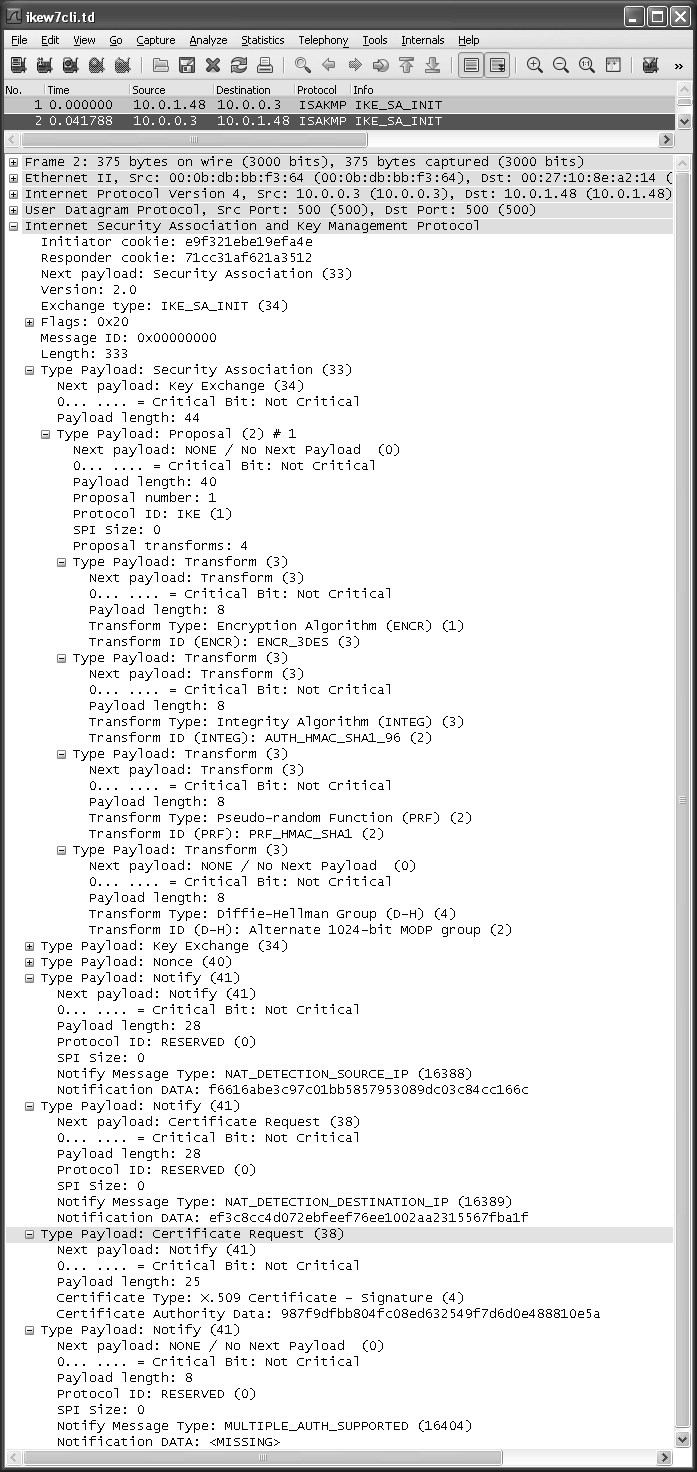
\includegraphics[width=0.7\textwidth]{imgs/18/18-23.png}
	\caption{SA\_INIT 交换包括响应者的SPI(标记次“cookie”)、与转换相关的唯一建议、DH参数、
            随机数值以及 NAT转换地址参数。这条消息还包括一个 CERTREQ 负载,用于指明并请求
            可接受的证书;一个通知负载,用于指明所支持的多个(成系列)认证方法}
\end{figure}

图 18-23 中剩余的数据包包含了加密的\verb|IKE_AUTH|消息。它们使用4500而不是500
作为源与目的端口号,并采用特的包含4字节0\href{https://www.rfc-editor.org/rfc/rfc3947}{[RFC3947]}的“非ESP 标记”封装,从
而指明流量是IKE而非ESP。标记与端口号还用于我们之前讨论的 INFORMATIONAL 交
换中。
如果提供合适的密钥与 SPI 值,Wireshark 能够解密已加密的IKE 流量。通过为Wireshark
提供 IKE 服务器上的日志跟踪文件副本(位于 Edit | Preferences | Protocols | ISAKMP 路径下),
我们能够查看加密的IKE 负载信息。(Wireshark 开发者倾向于使用协议的原始名称,比如用
ISAKMP 与 SSL代替IKE 与TLS,
因此 Wireshark 的输出结果也会使用这些名称。)
图18-22中的第3个数据包是UDP/IP 数据报的第一个分片。当接收到第2个分片(数
据包 4)后,Wireshark 将会重组这个数据报。图18-24显示了解密与重组后的结果。
\begin{figure}[!htb]
    \centering
	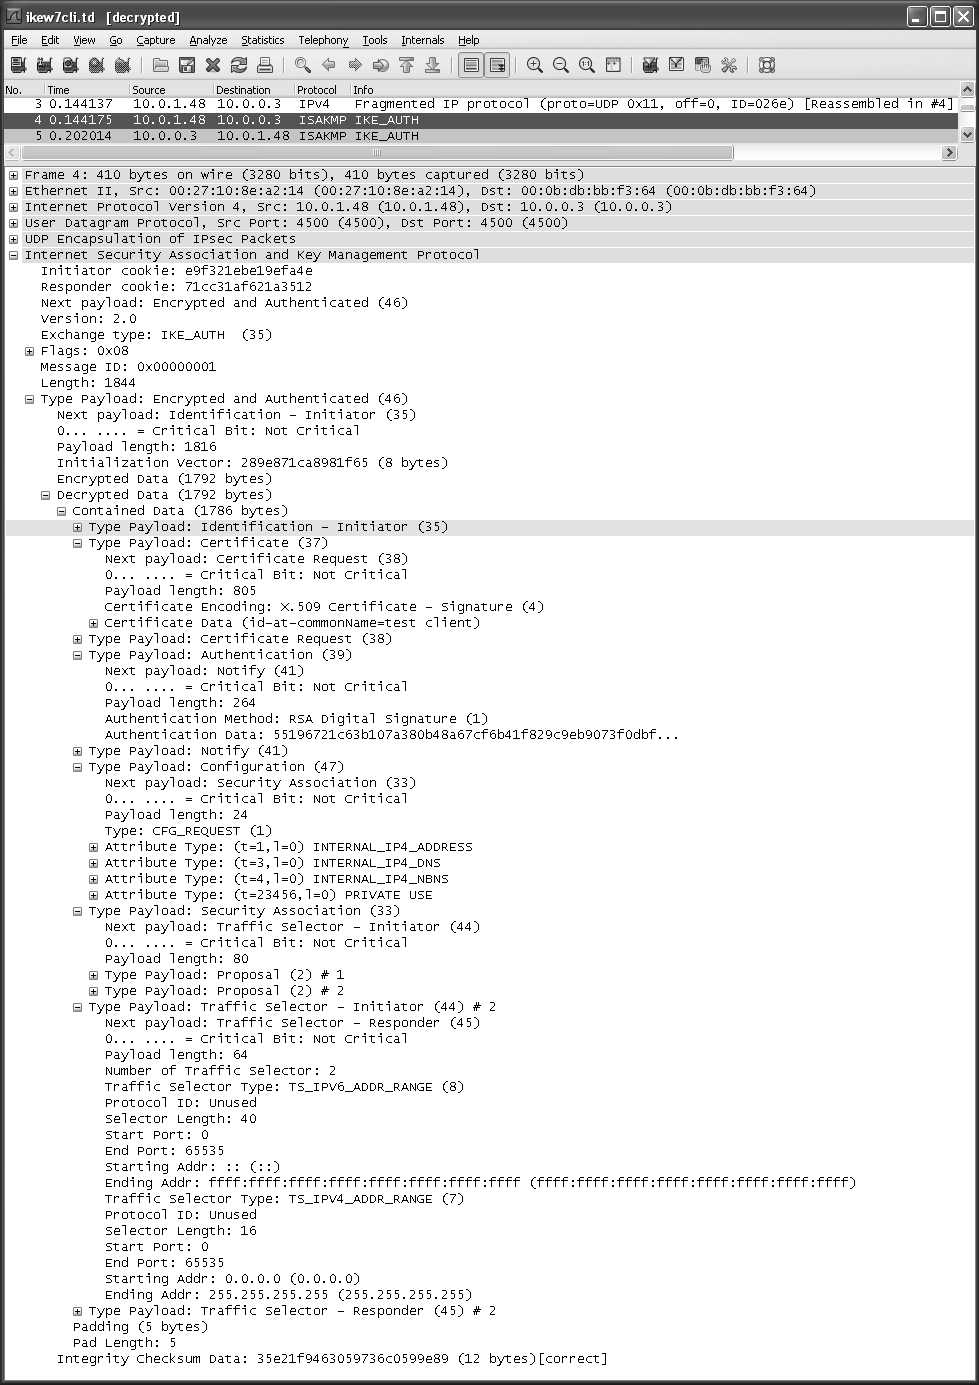
\includegraphics[width=0.7\textwidth]{imgs/18/18-24.png}
	\caption{IKE\_AUTH 交换包含加密信息,并运行在UDP 4500端口。通过重组2个分片可以生成一条
            带有加密/认证数据负载的IKE消息。这条消息包含以下负载:发起者标识符(IDi)、证书
            (CERT)、证书请求(CERTREQ)、认证(AUTH)、通知(N)、配置(CP)、安全关联(SA)、
            流量选择器发起者(TSi)以及流量选择器响应者(TSr)}
\end{figure}
图18-24

安全:可扩展身份认证协议、IP安全协议、传输层安全、DNS 安全、域名密钥识别邮件 619
UDP/IPv4分片在经过重组与解密之后,我们能看到\verb|IKE_AUTH| 交换中第一个数据包的
构成内容。客户端提供了下述IE负载:IDi、CERT、CERTREQ、AUTH、N(\verb|MOBIKE_SUPP|)、
CP、SA、TSi以及TSr。IDi负载包含了发起者与测试客户端的名称。CERT负
载包含了一个客户端证书。该证书是由测试证书颁发机构签署的,因此相关服务器会接
受(根据配置要求)。CERTREQ负载包含了对测试CA以及其他21个 Windows 7 客户端已
知的CA 的请求(这里未显示)。AUTH负载包含了一个使用发起者的 RSA私钥签名的数据
块(参见\href{https://www.rfc-editor.org/rfc/rfc5996}{[RFC5996]}的2.15节),它能够提供原始的认证。N(\verb|MOBIKE_SUPPORTED|)指明
客户端是否愿意遵循MOBIKE 协议。CP(\verb|CFG_REQUEST|)负载(未详细描述)包含了以下
属性:\verb|INTERNAL_IP4_ADDRESS|、\verb|INTERNAL_IP4_DNS|、\verb|INTERNAL_IP4_NBNS| 与一个
\verb|PRIVATE_USE| 类型(23456)。这些负载用于帮助配置 VPN访问,或者服务于DHCP 本地配
置信息等目的(参见第6章)。NBNS指的是一个 NetBIOS 名称服务器。NetBIOS 是一个可执
行在若干网络协议之上的API,并且在 Windows 环境下是通用的。

图18-24中的SA负载描述了构成\verb|CHILD_SA| 的信息。其中有两个建议(未详细描述),
每一个建议针对使用32位SPI 值的ESP(注意IKE使用64位的SPI值),它使用\verb|AUTH_HMAC_SHA1_96|
 作为完整性算法,并且不使用扩展序列号(指明使用建议转换)。第一
个建议提出使用\verb|ENCR_AES_CBC|(256位密钥)用于加密,而第二个建议则提出使用
\verb|ENCR_3DES|。由于没有提出 N(\verb|USE_TRANSPORT_MODE|)负载,我们认为每一条建议都会
在默认的隧道模式下使用ESP。

图18-24中的流量选择器(TSi 与TSr)负载指出允许用于形成 SA 的IPv4 与IPv6地址
范围。TSi 既包含 \verb|TS_IPv6_ADDR_RANGE|,又包含\verb|TS_IPv4_ADDR_RANGE|,这样就包含
了全部的地址与端口号范围。TSr(不详细描述)包含相同的值。
之前讨论的第一个 \verb|IKE_AUTH| 消息相对复杂并且需要不止一个1500字节的UDP/
IPv4 数据报。在响应者处理之后,会产生交换过程中的最终消息。图18-25展示了这条
消息。
在图18-25中,服务器发送的响应包含以下负载:IDT、CERT、AUTH、CP(\verb|CFG_REPLY|)、
SA、TSi、TSr、N(\verb|AUTH_LIFETIME|)、N(\verb|MOBIKE_ SUPPORTED|)以及N(\verb|NO_ADDITIONAL_ADDRESSES|)。
IDr 负载包含了一个DER编码的服务器名称。CERT 负载
包含了与之匹配的(服务器)证书。AUTH负载指出相关私钥的信息。CP(\verb|CFG_REPLY|)负
载包括一个用于VPN配置的\verb|INTERNAL_IP4_ADDRESS| 属性。SA负载与图18-24中客
户端的SA负载类似,并包含唯一一条能够实现 \verb|ENCR_AES_CBC|(256位密钥)、\verb|AUTH_HMAC_SHA1_96|
以及非ESN之间转换的建议。

数据包中TSi与TSr的数值被“压缩”在比客户端的\verb|IKE_AUTH| 消息更小的范围之
内。在这种情况下,TSi被限制在唯一的IPv4地址10.100.0.1,TSr 被限制在10.0.0.0/16。
它们都能够使用完全的端口范围0~65535。这是一个相对简单的压缩情况。在有些情况中
会出现多个由发起者指出的间断的范围子集,因此就需要生成一个 N(\verb|ADDITIONAL_TS_POSSIBLE|)
负载。使用压缩的方法是为 SA 人工地协商地址范围。

N(\verb|AUTH_LIFETIME|)负载指出认证过程将持续至多2.8小时(10 154秒,在跟踪文件
中表示为000027aa)。N(\verb|MOBIKE_SUPPORTED|)负载指出了响应者是否支持 MOBIKE协议。
\verb|NNO_ADDITIONAL_ADDRESSES|)负载(不详细描述)与MOBIKE 协议一起使用指出除
了交换中使用的地址之外不再需要额外的IP 地址。
\begin{figure}[!htb]
    \centering
	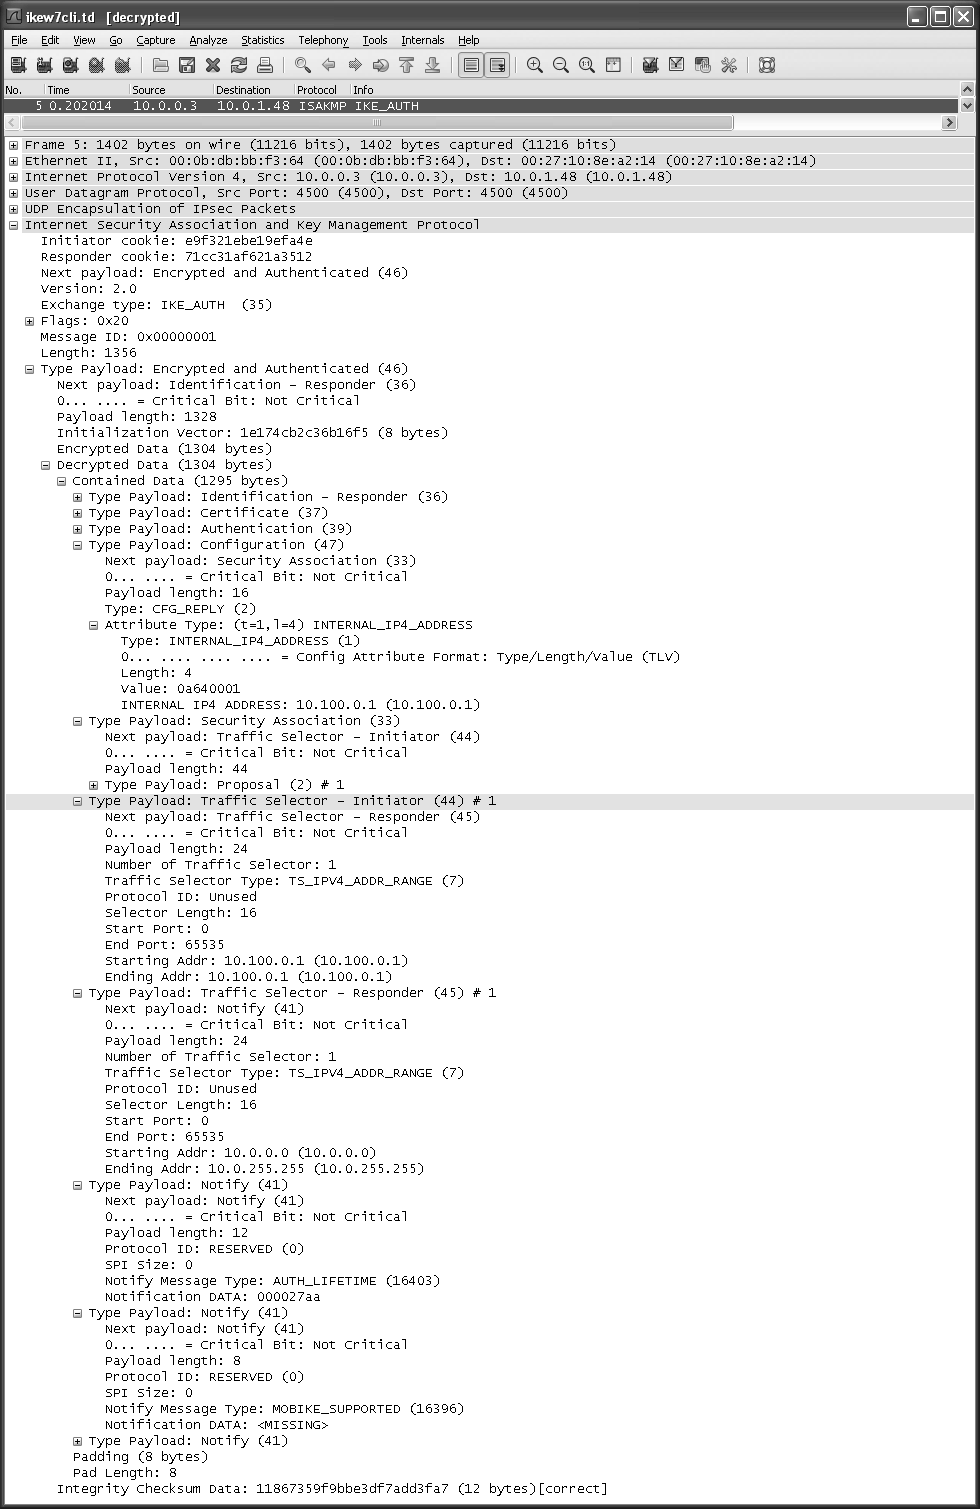
\includegraphics[width=0.7\textwidth]{imgs/18/18-25.png}
	\caption{在完成 IKE\_AUTH 交换过程中,响应者产生一个已加密/认证的数据负载。该负载包含以下
            负载:响应者标识符(IDr)、CERT、AUTH、CP(CFG\_REPLY)、SA、压缩的TSi与TSR,以
            及 N(AUTHL LIFETIME)、NCMOBIKE\_SUPPORTED) 和 NONO\_ADDITTIONAL\_ADDRESSES)。
            第一个 CHILD\_SA 现在可以开始操作}
\end{figure}

至此,一个隧道模式的ESP \verb|CHILD_SA| 已成功建立,并且数据流能够得到传输。我们
安全:可扩展身份认证协议、IP 安全协议、传输层安全、DNS 安全、域名密钥识别邮件 621
不再详细地介绍包含 ESP数据包的流量(它们相对简单),而是跳至SA的删除。它是通过两
套包含删除负载的 INFORMATIONAL 交换实现的,其中一个用于 ESP SA,而另一个用于
IKE SA。图18-26展示了关闭ESP SA 的请求。
\begin{figure}[!htb]
    \centering
	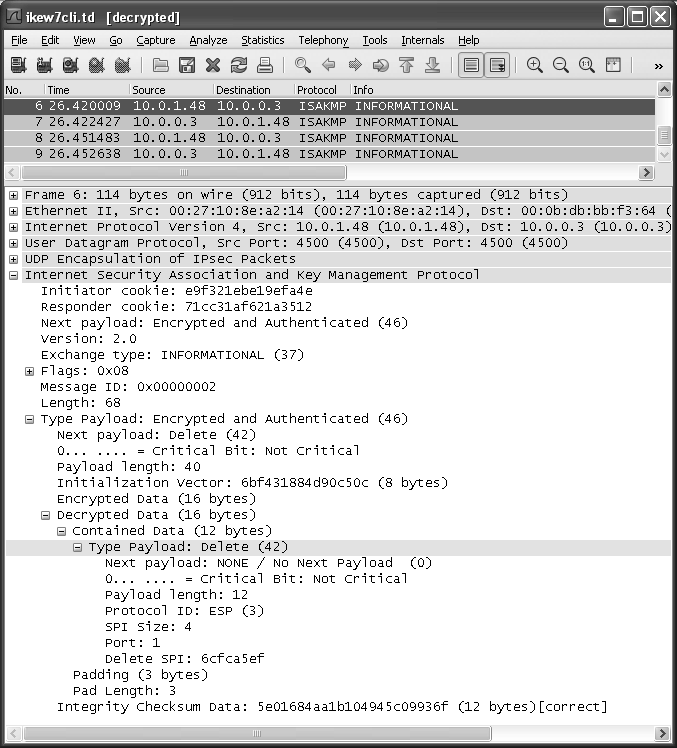
\includegraphics[width=0.7\textwidth]{imgs/18/18-26.png}
	\caption{删除子 ESP SA 的请求(通过在 IKE SA 中包含 SPI 值 6cfcaSef)。删除负载显示端口号为1,
            Wireshark 并没有对此进行标记(它应该是 SPI 的数值:1)}
\end{figure}

在图 18-26中可以看到,将要删除的SA 基于一个来自客户端的关闭请求。与其他IKE
数据流类似,它包含了一个已加密与认证的负载。这个加密的负载依次包含了一个删除负
载。删除负载可指出不止一个 SPI 将被删除,但在本例中它指的是数值为 Ox6cfcaSef的 SPIo
来自响应者的数据包7大致相同,但是在标志位字段拥有不同的设置(响应者代替发起者,
响应代替请求),同时在加密IV 与完整性校验数据部分也有不同的内容。数据包7还在删除
负载部分指出了一个不同的SPI(数值內c348faf2)。
要关闭 IKE-SA,还需要另一个 INFORMATIONAL 消息的交换。发起者首先发送图
18-27中的数据包。我们可以看到一个关闭IKE SA 的请求。删除负载需要与其他流量一样
进行加密,但是因为是通过IKE SA 来传输删除请求,所以不需要包含一个 SPI数值。为
了完成IKE SA删除,响应者将在数据包9中包含一个空的加密/认证负载类型的IKE消
息。它的下一个负载类型字段设置为NONE(0)。这样就表明已经完成了 IKE SA 的删除。
875
622
第18章
\begin{figure}[!htb]
    \centering
	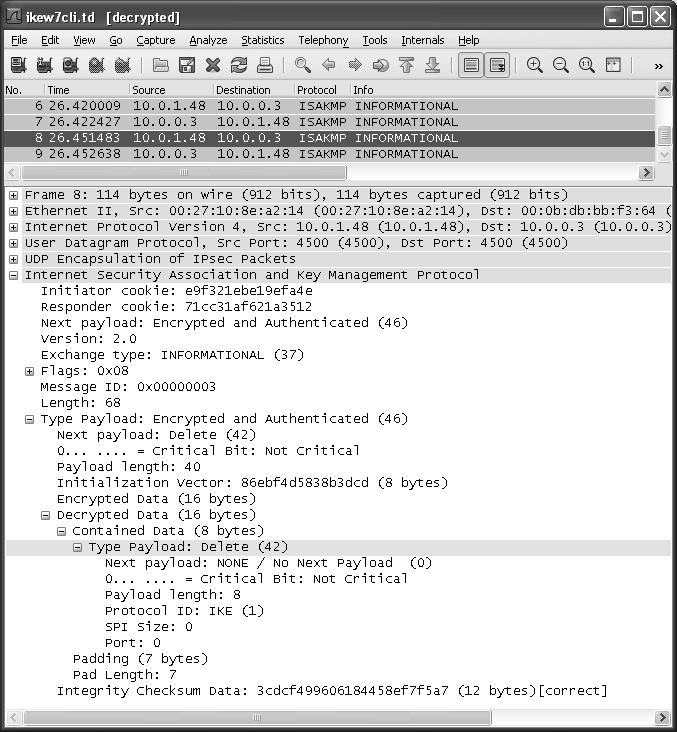
\includegraphics[width=0.7\textwidth]{imgs/18/18-27.png}
	\caption{删除 IKE SA 的请求。由于整条消息都是通过 IKE SA 传输的,
            所以不需要SPI 数值,而且不会存在不明确之处}
\end{figure}

\section{传输层安全(TLS 和 DTLS)}
之前已经讨论过第2层与第3层的安全协议。运行在传输层之上的最流行的安全协议是
传输层安全(Transport Layer Security,TLs)。TLS 用于保证 Web 通信以及其他流行协议的
安全,比如POP、IMAP(当使用TLS保护后,它们被分别称为POP3S与IMAPS)。TLS 流
行的一个原因是它能够在应用程序内部或底部实现,而这些应用程序是运行于底层之上的。
一些协议比如 EAP与 IPsec通常要求在操作系统内部或者主机与嵌人式设备的协议上来实现
功能。

TLS 以及它的前身安全套接字层(Secure Sockets Layer,SSL \href{https://www.rfc-editor.org/rfc/rfc6101}{[RFC6101]}) 有多个版本。
本书将关注最近起草的 TLS 1.2版本\href{https://www.rfc-editor.org/rfc/rfc5264}{[RFC5264]}。TLS 1.2支持向下兼容大多数旧版本的 TLS
与 SSL(例如,TLS 1.0,1.1以及 SSL3.0)然而,TLS 1.2对SSL 2.0的支持较弱,但是它们
之间的互操作是可以实现的。现在SSL 2.0已经禁止使用\href{https://www.rfc-editor.org/rfc/rfc6176}{[RFC6176]}。TLS 1.2运行在面向流
的协议(通常为 TCP)之上。在完成对它的讨论之后,本书将介绍面向数据报的版本,称为
数据报传输层安全(DatagramTransport Layer Security,DTLS \href{https://www.rfc-editor.org/rfc/rfc4347}{[RFC4347]})。DTLS正逐步在
一些不使用 IPsec 的应用程序中流行起来,比如VPN实现。它当前的草案是基于 TLS1.1版
本\href{https://www.rfc-editor.org/rfc/rfc4346}{[RFC4346]},但是更新工作也正在进行中[IDDTLS]。

\subsection{TLS 1.2}
TLS 的安全目标与 IPsec类似,但TLS运行在更高的层次之上。它在多种加密套件的基
础上提供机密性与数据完整性(这些加密套件往往会使用PKI提供的证书)。TLS 还能够在
两个匿名通信方之间建立安全连接(不使用证书),但这一应用很容易受到 MITM 攻击(由
于双方没有更好地进行身份识别,所以受到此类攻击也不足为奇)。TLS 协议本身分为两层,
称为记录层与上层。记录协议实现记录(下)层,并假设位于一个可靠的底层协议之上(例
如TCP)。图 18-28展示了基本的组织形式。
\begin{verbatim}
    密码变更
    协议
    警告协议
    握手协议
    应用数据
    协议
    上层
    协议
    分片
    压缩
    加密与完整性保护
    记录层
    (记录协议)
\end{verbatim}
图 18-28
TLS协议“栈”包括位于底部的记录层以及上层协议(称为信息交换协议)中的三个协议。
第4个上层协议是使用TLS的应用协议。记录层提供分片、压缩、完整性保护以及加密功
能。握手协议 TLS 完成的许多工作类似于IKE 为 IPsec 所做的工作
TLS是一个客户端/服务器协议,设计用于为两个应用程序的连接提供安全。记录协议
提供分片、压缩、完整性保护以及对客户端与服务器之间所交换数据的加密服务。信息交换
(handshaking)协议负责建立身份、进行认证、提示警报,以及用于每一条连接的记录协
议提供唯一的密钥材料。信息交换协议包含了4个特殊的协议:握手协议、警告协议、密码
变更协议以及应用数据协议。与IPsec类似,TLS 是可扩展的,能容纳当前或未来的加密套
件—TLS 称其为密码套件(Cipher Suite,CS)。目前已经定义了多种组合,IANA 维护了
当前集合的注册表[TLSPARMS]。当前 TLS 的版本都基于 SSL 3.0,源自 Netscape。 TLS与
SSL 并不能直接进行互操作,但是一些协商机制允许客户端与服务器在连接首次建立时动态
地发现该使用哪一种协议。
密码变更协议用于改变当前运行的参数。它首先通过握手协议建立 “挂起”状态,随后
通过一个指示从当前状态切换至挂起状态(稍后又会返回当前状态)。这些切换只有在挂起
状态准备完毕后才被允许。TLS 基于5个加密操作:数字签名、流密码加密、分组密码加密、
认证加密相关的数据(AEAD)以及公钥加密。为实现完整性保护,TLS 记录层使用基于散
列的消息认证码(HMAC)。为生成密钥,TLS 1.2使用一个基于HMAC(它采用SHA-256
算法)的伪随机函数族(PRF)。TLS 还整合了一个可选的压缩算法——该算法在连接首次建
立时由双方协商。

\subsubsection{TLS 记录协议}
记录协议使用一个可扩展的记录内容类型值集合来识别可多路复用的消息类型(即高层
协议是哪一种)。在任何给定的时间点,记录协议有一个活跃的当前连接状态和一组被称为
挂起连接状态的状态参数。每一个连接状态又进一步被划分为读状态与写状态。每一个状态
都会指定一个压缩算法、加密算法以及用于通信的MAC算法,同时还包括必需的密钥与参
数。当一个密钥被交换时,TLS 首先会使用握手协议建立挂起状态,然后通过一个同步操作
(通常使用密码变更协议完成)将当前状态设置为挂起状态。当首次被初始化时,所有状态被
设置为未加密、未压缩以及无 MAC过程。

记录协议的处理流程如图18-29所示。它将高层信息块(分片)划分为称作TLS明文
记录的记录。该记录最长为24字节(但通常远小于这个数值)。对记录大小的选择仍保留
在TLS中,高层消息的边界不会被保留。TLS明文记录一旦形成,就会使用一种能在当前
连接状态中识别的压缩算法\href{https://www.rfc-editor.org/rfc/rfc3749}{[RFC3749]}进行压缩。总有一种压缩协议是有效的,虽然它可能
(通常)是 NULL压缩协议(不提供任何压缩也不足为奇)。压缩算法将TLS明文记录转换为
TLS压缩结构。压缩算法应该是无损的,产生的输出结果不能大于输入记录1KB。为了防止
负载被披露或修改,加密与完整性保护算法会将 TLS压缩结构转换为能够在底层传输层连接
上发送的 TLS 密文结构。

\begin{verbatim}
    0
    15 16
    内容类型(8位)
    主要版本(8位)次要版本(8位) 长度(高8位)
    长度(低8位)
    负载分片
    (可变,最大2 4字节)
    0
    内容类型(8位)
    15 16
    主要版本(8位)次要版本(8位)
    长度(高8位)
    长度(低8位)
    31
    从高(上)层
    TLS明文
    31
    压缩
    (可选)
    压缩负载分片
    (可变,最大1024+2 字节)
    TLS压缩结构
    0
    内容类型(8位)
    长度(低8位)
    1516
    主要版本(8位)
    次要版本(8位)
    已加密/受保护的负载
    (加密+MAC+[填充/填充长度])或
    (随机数+被签名加密部分)
    31
    加密/证
    长度(高8位)
    / TLS密文
    发送至传输层
\end{verbatim}
图18-29
TLS记录层开始于TLS明文记录。它通过一个无损的压缩算法生成一个TLS 压缩记录。
TLS压缩记录经过加密(包括 MAC)生成一个可用于传输的TLS密文记录。传统的流或分
组密码要求一个 MAC,分组密码可能会包含填充数据。当使用AEAD 密码时,加密与完整
性保护的内容中会包含一个随机数,并且不需要单独的 MAC
参照图 18-29,当产生一个 TLS密文结构时,首先会计算一个序列号(但不放在消息
中),然后会根据需要计算一个消息认证码(MAC),最后进行对称加密。在加密之前,消
息可能会被填充(多达255字节)以满足加密算法所要求的分组长度(例如,分组加密)。
AEAD算法(例如,CCM、GCM)不需要MAC 就能够提供完整性保护与加密功能,但它需
要一个随机数。
记录协议的密钥源自于一个主密钥(master secret)——它是通过记录协议之外的其他方
法提供的,绝大多数情况下使用握手协议。根据主密钥以及在连接开始时由客户端与服务器
应用程序提供的随机值可以生成下面的密钥:
\begin{equation}
    , = PRF(master_secret, "key expansion",
    server_random + client_random)
\end{equation}
在上述表达式中,“|”是分隔运算符,“+”是连接运算符。M。表示用于客户端的 MAC
写密钥,Ms表示用于服务器的MAC写密钥,D。表示客户端的数据写密钥,D。表示服务
器的数据写密钥,IV。表示客户端的初始向量(IV),IV。表示服务器的初始向量。通过“|”
运算符,每个密钥使用了 PRF函数要求的多个字节。MAC、加密以及IV 密钥在使用时会
根据选择的加密套件而固定长度。最后两个值只用于 AEAD加密中隐式地产生随机数(参
见[RFCS116]3.2.1节)。根据\href{https://www.rfc-editor.org/rfc/rfc5246}{[RFC5246]},加密套件需要的最常见材料是 \verb|AES_256_CBC-SHA256|。
它要求4个32字节的密钥,合计128字节。

\subsubsection{TLS 信息交换协议}
TLS有3个子协议,它们的主要任务与IPsec中的IKE大致相同。更具体地说,这些协
议是通过数字分辨的。这些数字被记录层用于多路复用与多路分解,比如握手协议(22)、
警告协议(21)、密码变更协议(20)。密码变更协议非常简单。它包括一个单字节的消息,
该字节的数值为1。该消息的目的在于指出通信一方希望将当前状态修改为挂起状态。如果
收到这条消息,就将读挂起状态作为当前状态,并指示记录层尽快转换至挂起写状态。这条
消息将同时用于客户端与服务器。

警告协议用于从TLS连接的一端向另一端传递状态信息。它可以包括一些终止条件(无
论是致命的错误或是可控的关机)或非致命的错误条件。在公布的\href{https://www.rfc-editor.org/rfc/rfc5246}{[RFC5246]}中,将24条
警告消息定义为标准。其中有超过一半的消息始终是致命的(例如,坏的MAC、丢失或来
历不明的消息、算法故障)。

握手协议建立了与连接相关的运行参数。它允许 TLS端点完成6个主要目标:协商加
密算法并交换形成对称密钥时使用的随机值;建立算法运行参数;交换证书并执行互相认证;
生成特定的会话密钥;为记录层提供安全参数;验证所有的操作都已正确执行。图18-30展
示了需要的消息。

图18-30展示的握手过程是以 Hello消息开始的。通常由客户端向服务器发送第一条
客户端Hello(ClientHello)消息。该消息包含一个会话标识符、建议的加密套件编号(图
18-30中的CS)以及一套可接受的压缩算法(虽然\href{https://www.rfc-editor.org/rfc/rfc3749}{[RFC3749]}也定义了 DEFLATE,但通常
为NULL)。TLS 支持超过250个加密套件选项 [TLSPARAMS]。

客户端Hello 消息还包含 TLS的版本号与一个称为 ClientHello.random 的随机数。接收
到客户端 Hello消息,服务器会检查其中的会话标识符是否在其缓存中。若是,则服务器可
能会通过一个简化的握手过程继续之前已有的连接(称为“重新开始”)。该简化的握手过
程是影响 TLS性能的关键。它可以避免重复认证端点身份的工作,但它也要求通信两端具
有相同的密码协议。服务器 Hello (ServerHello)消息通过将服务器的随机数(ServerHello.
random)传递至客户端完成了交换的第一部分。这条消息也包含了一个会话标识符。如果它
的数值与客户端的数值相同,则表明服务器愿意重新开始。否则,它的数值为0表示需要开
启一个完整的握手过程。

如果执行一个完整的(无简化)握手过程,交换Hello消息会使得每一端都能够了解加
密套件、压缩算法以及它们的随机值。服务器会在客户端指出的加密套件中进行选择。如果
服务器需要通过身份验证,会要求它在证书(Certificate)消息中提供自己的证书链(这是安
全Web 与HTTPS中的典型情况)。如果证书的签名是无效的,那么服务器可能还需要发送
一个服务器密钥交换消息,使其在没有证书的情况下通过一个暂时的或短暂的密钥生成会话
\begin{verbatim}
    密钥。
    客户端
    服务噩
    简化的握手
    (重新开始)
    ClientHello
    (session ID, CS, Comp)
    {extensions}
    ServerHello
    -(session ID, CS, Comp)-
    {extensions}
    - Certificate(Server)
    ServerKeyExchange
    CerificateRequest
    -ServerHelloDone.
    Certificate (Client)
    - ClientKeyExchange
    -CertificateVerify-
    [ChangeCipherSpec]
    -Finished-
    简化的握手
    (重新开始)
    -[ChangeCipherSpec]
    - Finished
    数据交换(受保护的)
    图18-30
\end{verbatim}
正常的 TLS连接初始交换包括若干条消息,按流水线的方式排列。需要的消息用实心箭头
与黑体字表示。如果之前存在的连接能够重新启动,那么就使用简化的交换过程。这样就避
免了端点的认证工作,使处理能力有限的系统能够节省资源
\begin{tcolorbox}
    服务器密钥交换消息(ServerKeyExchange)仅用于证书(服务器)消息没有包
    含足够的信息来建立预置密钥(premaster secret) 的情况。这种情况包括匿名或短暂
    的 DH 密钥协议(即密码套件以\verb|TLS_LDHE_anon|、\verb|TLS_DHE_DSS| 以及 \verb|TLS_DHE_RSA|
    开头)。服务器密钥交换消息不用于其他套件,包括那些以 \verb|TLS_RSA|、\verb|TLS_DH_DSS| 或 \verb|TLS_DH_RSA| 开头的套件。
\end{tcolorbox}
此时,服务器可能会要求对客户端进行身份验证。如果是这样,它将会产生一个
证书请求消息。一旦这条消息发送出去,服务器通过发送强制性的服务器Hello完成
(ServerHelloDone)消息完成交换的第二部分。当接收到来自服务器的这一条消息(可能是
管道传输的),客户端可能会被要求证明自己的身份(即,拥有与证书相对应的密钥)。如果
是这样,它首先通过一条与服务器格式相同的证书消息发送自己的证书,然后发送强制性的
客户端密钥交换(ClientKeyExchange)消息。这条消息的内容依赖于使用的密码套件,但它
通常包含一个 RSA加密的密钥,或用于创建新密钥种子的 Diffie-Hellman 协议参数(被称
预置密钥)。最后,它发送一个证书验证(CertificateVerify)消息以证明在服务器要求客户端
验证身份的情况下自己拥有与之前提供的证书对应的私钥。这条消息包含对一个散列值的签
名。该散列值是根据客户端之前收到的以及发送的所有握手消息生成出来的。

交换的最后一部分包含一个修改密码协议(ChangeCipherSpec)消息,这是一个独立的
TLS 协议内容类型(即,从技术上看不是一个握手协议消息)。然而,只能在成功交换修改
密码协议消息后才能进一步交换强制性的握手协议已完成(Finished)消息。已完成消息是迄
今为止第一批通过使用已交换的参数来保护的消息。已完成消息本身包含“验证数据”,由
下面的值组成:

\begin{equation}
    verify_data = PRF(master_secret, finished_label, Hash(handshake_messages))
\end{equation}

其中 \verb|finished_label| 可取两个值,值 “client finished”用于客户端,而值 “server finished”
用于服务器。特定的散列函数Hash与在初始Hello消息交换阶段PRF的选择密切相关。
TLS 1.2 提供了可变长度的验证数据,但是之前所有的版本与当前加密套件都产生12字节的
验证数据。48字节的 \verb|master_secret| 值根据下式进行计算:
\begin{equation}
    master_secret = PRF(premaster secret, "master secret",
    ClientHello.random + ServerHello.random)
\end{equation}
此处+是连接运算符。已完成消息是十分重要的,这是由于它在很高程度上证实了握手协议
已经成功完成,并允许之后的数据交换。

\subsubsection{TLS扩展}
迄今止,本书已经介绍了IKE与TLS。如果比较它们的功能,我们会发现IKE 携带
的信息能够超出建立基本SA所需的信息。这是通过使用IKE 通知与配置负载完成的。为
了提供类似的扩展机制,TLS 1.2消息以一种标准的方式包含了多种扩展。TLS的基准规范
\href{https://www.rfc-editor.org/rfc/rfc5246}{[RFC5246]}包括一个“签名算法” 扩展。这样客户可以用它来为服务器指出自己可提供的散
列与签名算法类型(用于散列的MDS、SHA-1、SHA-224、SHA-256、SHA-384、SHA-512
以及用于数字签名的RSA、DSA、ECDSA)。由于一些系统只允许特定的组合,这些扩展会
按照偏好程度降序排列。文档[TLSEXT]给出了当前的扩展列表。

TLS之前的版本大约有6个扩展,\href{https://www.rfc-editor.org/rfc/rfc6066}{[RFC6066]}将这些扩展都更新至TLS 1.2中。它定义
了下列扩展:\verb|server_name|(按照 DNS风格显示的服务器名称),\verb|max_fragment_length|(一条
消息的最大长度为2'字节,n的值为9~12),\verb|client_certificate_url|(指明支持证书URL 握
手消息,该消息用于发送证书的URL 而不是一个完整的证书),\verb|trusted_ca_keys|(散列值,或
受信任的CA公钥名称以及证书),\verb|truncated_hmac|(只使用HMAC的前80位进行计算),以
及 \verb|status_request|(请求服务器使用OCSP协议,并在证书状态握手消息中提供DER编码的
响应来验证一个证书)。每一个扩展都可能出现在一个(扩展的)客户端Hello消息中,在某
些情况下可能会出现在服务器Hello消息中来表示同意。除了这些扩展与已经提到的两个握
手消息,\href{https://www.rfc-editor.org/rfc/rfc6066}{[RFC6066]}还定义了4个警告消息:\verb|certificate_unobtainable|、\verb|unrecognized_name|、
\verb|L_certificate_status_response| 以及 \verb|bad_certificate_hash_value|。它们都是自说明的,除非节
点已经证明能够理解扩展的客户端Hello类型消息,否则它们不会被发送出去。
其他几个扩展也已被定义或保留。\verb|user_mapping| 扩展\href{https://www.rfc-editor.org/rfc/rfc4681}{[RFC4681]} 提供了一种用户标
识符(例如,Windows 域)提供内容的方法。另一个 \verb|cert_type| 扩展不仅包括X.509证书,还
包括 OpenPGP 证书\href{https://www.rfc-editor.org/rfc/rfc6091}{[RFC6091]}。信息文档\href{https://www.rfc-editor.org/rfc/rfc4492}{[RFC4492]}描述了椭圆曲线密码套件。根据信息
文档\href{https://www.rfc-editor.org/rfc/rfc5054}{[RFC5054]}定义的方法,安全远程密码协议(Secure Remote Password protocol, SRP)
能够与TLS结合。\href{https://www.rfc-editor.org/rfc/rfc5764}{[RFC5764]}定义了一个 \verb|use_srtp |扩展,该扩展被设计用于生成一个基于
DTLS(参见18.9.2节)的安全实时协议(Secure Real-Time Protocol, SRTP)。 SessionTicket
TLS扩展\href{https://www.rfc-editor.org/rfc/rfc5077}{[RFC5077]}定义了一种方法,用于消除服务器上必须存储的用于恢复会话的状态。
它涉及将必要的状态以一种加密形式放人客户端中。最后,一个重要的\verb|renegotiation_info| 扩
展用于应对重新协商的漏洞。我们将在下面的章节对其进行详细介绍。

\subsubsection{重新协商}
TLS 支持在保持同一连接的同时重新协商加密连接参数。这一功能能够通过服务器或客
户端发起。如果服务器希望重新协商连接参数,它会生成一个 Hello 请求消息,而客户端会
响应一个客户端Hello消息以开启重新协商过程。客户端也能够自发地生成一个客户端Hello
消息,而无须服务器的提示。

虽然是否支持重新协商是可选的,但“强烈推荐”使用,例如,在对序列号进行封装的
情况下。可以通过生成一个 \verb|no_renegotiation|(类型100)警告来拒绝进行协商。虽然这类警
告不要求终止连接,但根据本地策略在收到它们之后将会终止连接。

2009年,一个使用重新协商功能的TLS攻击被成功实施。我们将会在18.12节对其
进行详细描述。这一漏洞允许攻击者与服务器建立一个恶意的TLS会话。客户端能够通过
MITM攻击将该会话转接到一个后续的合法会话中。服务器只会认为发生了一个符合标准的
重新协商。\href{https://www.rfc-editor.org/rfc/rfc5764}{[RFC5764]}给出了这一问题的解决方案,即利用一个称为 \verb|renegotiation_info|(类
型 0xffO1)的TLS扩展将重新协商与当前会话更紧密地绑定在一起。当创建一个新连接时,
\verb|renegotiation_info| 扩展为空,当客户端进行重新协商时,它包含 \verb|client_verify_data|;而当服
务器进行重新协商时,它包含 \verb|client_verify_data| 以及 \verb|server_verify_datao| \verb|client_verity_data|
是客户端在完成最后一次握手时所发送的已完成消息中包含的\verb|verify_data|。在TLS 中,这是
一个 12字节的数值(SSL v3 中36字节)。\verb|server_verify_data| 是服务器在完成最后一次握
手时所发送的已完成消息中的\verb|verify_data|。

一些已部署 TLS(与SSL)的服务器会在出现未知扩展时终止连接。为了在部署(相对
新的)renegotiationinfo 扩展时能够处理这一问题,需要提供另一种可用选择。在连接建
立过程中,TLS密码套件 \verb|TLS_EMPTY_RENEGOTIATION_INFO.SCSV| 可用于指出一个
空 \verb|renegotiation_info| 扩展的等价情况。它使用一个信号密码套件值(Signaling Cipher Suite
Value,SCSV)来指出一组特定的功能,而不是去编码真正的密码套件(类似的方法还用在
DNSSEC 中用于 NSEC3记录,参见18.10.1.3节)。
\subsubsection{示例}
在图18-31的例子中,我们能够看到在连接建立过程中使用TLS 1.2 时交换的消息,该
过程会在本地环回接口上使用TCP/IP。客户端与服务器都有RSA证书,并将它们提供给通
信对方。初始的TCP握手与窗口更新以及127.0.0.1的源与目的IPv4地址都没有显示出来。
为了更清楚地表达,跟踪过程已用左右箭头进行注释。指向右边的箭头表明TCP报文段至
少包含一个 TLS消息,该消息由客户端发往服务器。指向左边的箭头表示消息是从服务器发
往客户端。为了显示这些输出结果,我们首先通过在 Analyze | Decode As ...菜单下选择 SSL
来要求 Wireshark 软件解码跟踪记录。

如图18-31所示,在初始的TCP层握手之后,TLS 交换开始于一个客户端Hello 消息。
纯的TCP ACK 穿插于TLS消息中。在修改密码协议消息被处理之后,后续信息开始被加
密。为了更详细地查看发生的细节,我们将展开前面若干个TLS 消息。图18-32展示客户端
Hello 消息的细节内容。

安全:可扩展身份认证协议、IP安全协议、传输层安全、DNS 安全、域名密钥识别邮件 629
\begin{figure}[!htb]
    \centering
	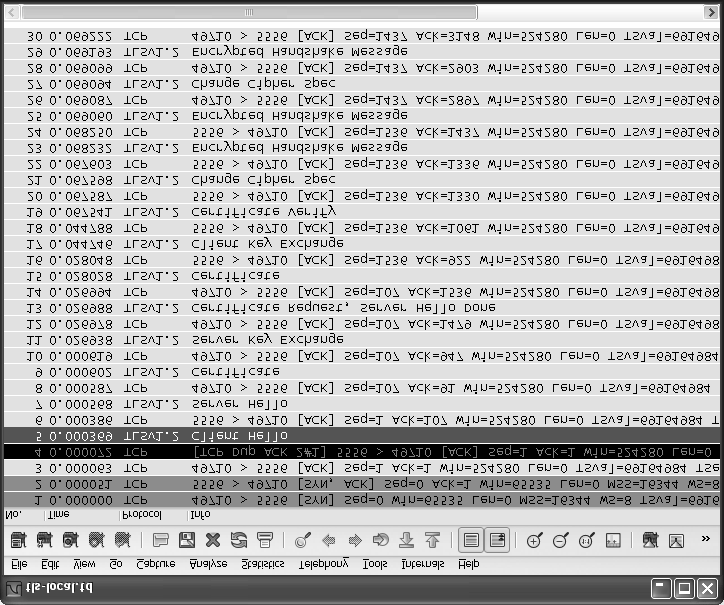
\includegraphics[width=0.7\textwidth]{imgs/18/18-31.png}
	\caption{利用 Wireshark 软件显示了一个正常的TLS 1.2 连接建立过程。服务器运行在5556端口。发
            送给服务器的客户端消息由指向右边的箭头标记。发送给客户端的服务器消息由指向左边的
            箭头标记。TCP的ACK 穿插于 TLS 消息中。在修改密码协议消息(报文段21)之后,其他
            的消息被加密与认证。报文段 13还包含 ServerHelloDone 消息}
\end{figure}
图 18-32详述的客户端Hello消息是一条承载 ClientHello 握手消息的记录协议消息。它
包含一个32位的UNIX时间戳,以秒为单位,从1970年1月1日的午夜12点开始计时。
此外,客户端Hello 消息还包含一个随机的28字节数值(ClientHello.random)用于形成密
钥。由于这是一个全新的连接,它的会话ID 为0。6个字节专门用于承载客户端支持的3个
密码套件,并按照推荐程度排序(最优推荐排在最前面)。每一套件都使用一个16位的数
值进行编码,该数值由[TLSPARAMS]中的TLS密码套件注册表指定。图中消息只支持一
种压缩方法—NULL 方法。该方法不会产生任何压缩结果,并已成为一种典型情况。此
外,消息还包含50个字节用于扩展。\verb|cert_type| 扩展指出使用的是X.509证书还是 OpenPGP
证书。\verb|server_name|扩展包含服务器提供给客户端应用程序的名称127.0.0.1。由于是第一次
握手,\verb|renegotiation_info| 扩展为空。SessionTicket TLS扩展也属于相同的情况。\verb|signature_algorithms|
扩展指出客户端能够处理的算法集合:shal-rsa、shal-dsa、sha256-rsa、sha384-
rsa 以及 sha512-rsa。

在这个简单的交换中,服务器被配置为只有一个密码套件:\verb|TLS_DHE_RSA_WITH_AES_256_CBC_SHA256|(0x006b)。
如图18-33所示,当通过一个服务器 Hello消息来响应客户端 Hello 消息时,服务器会指明这一事实。

在图18-33中,服务器用一条服务器 Hello 消息来响应客户端Hello 消息。服务器会提
供它的当前时间副本以及一个28字节的随机值。它还包括一个随机的32字节的会话ID。
服务器只支持一个密码套件(使用RSA证书的DH密钥协商,CBC模式的AES-256算法用
于加密,SHA-256算法用于完整性保护)。与客户端类似,服务器不支持任何压缩算法。服
务器还包含一个空的 \verb|renegotiation_info|与一个空的 SessionTicket TLS 扩展。在第一条消息之
后,服务器会继续发送一条证书消息,如图 18-34所示。
\begin{figure}[!htb]
    \centering
	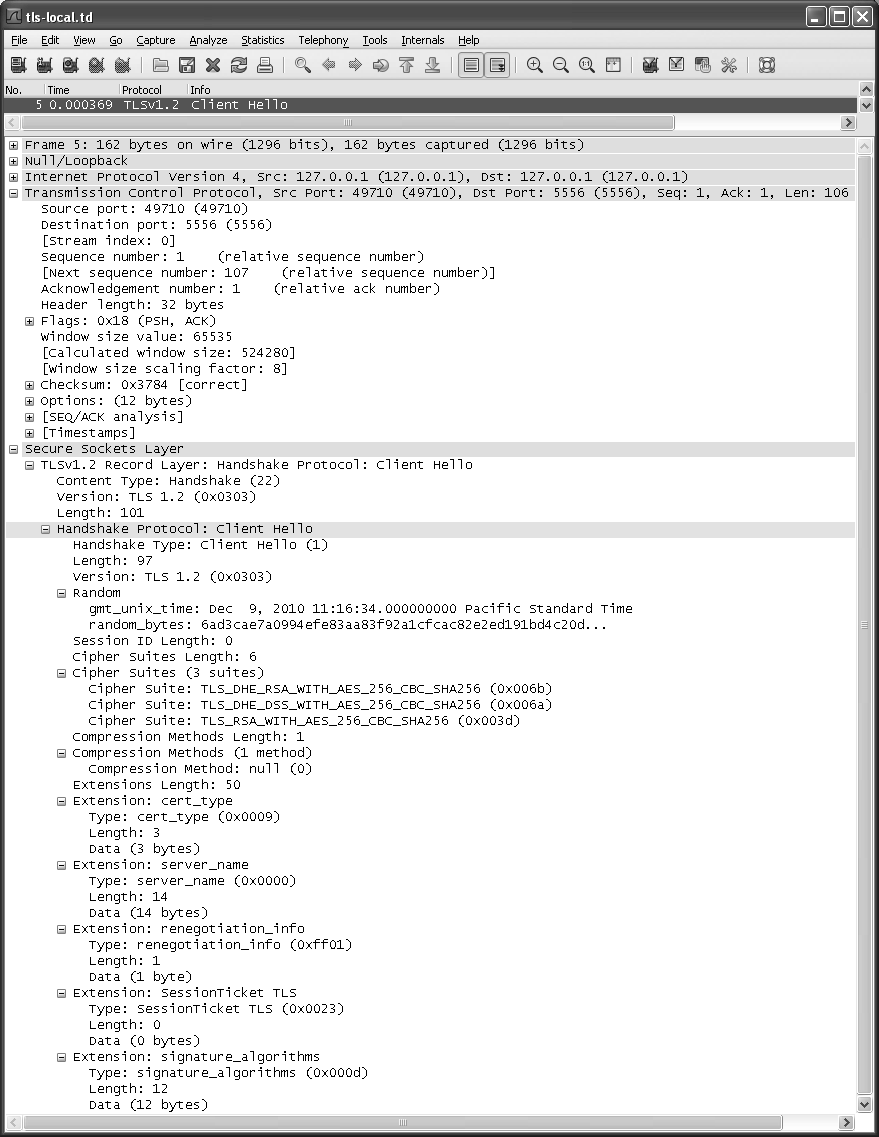
\includegraphics[width=0.7\textwidth]{imgs/18/18-32.png}
	\caption{TLS 1.2中一个客户端Hello 消息包括版本信息、所支持的密码套件与压缩算法、随机数据
            以及一些扩展。此处客户端支持 Diffie-Hellman 密钥协议以及使用RSA 的密钥交换。它使
            用CBC模式的AES-256算法用于加密,SHA-256算法用于完整性保护}
\end{figure}

图18-34中的消息将服务器的841字节的X.509v3证书传输至客户端。它是由一个称
为测试CA的样本证书颁发机构签署的。测试CA位于发布者(Issuer)字段。该字段被称力
SubjectPublickeyInfo,包含了服务器的270字节的RSA公钥。客户端会使用它来完成对服
安全:可扩展身份认证协议、IP安全协议、传输层安全、DNS 安全、域名密钥识别邮件 631
务器的身份认证。证书中有6个扩展:basicConstraints(关键的)、subjectAltame(包含使
用证书的服务器的DNS名称)、extKeyUsage(扩展的密钥用途,指出密钥的用途在于认证
服务器的身份)、keyUsage(关键的,指出可能用于密钥加密或生成数字签名的已关闭密钥)、
subjectKeyIdentifier(一个20字节的数字,用于识别已签名的公钥)以及 authorityKeyIdentifier
(一个20字节的数字,用于识别证书颁发机构用来生成当前证书的密钥)。

\begin{figure}[!htb]
    \centering
	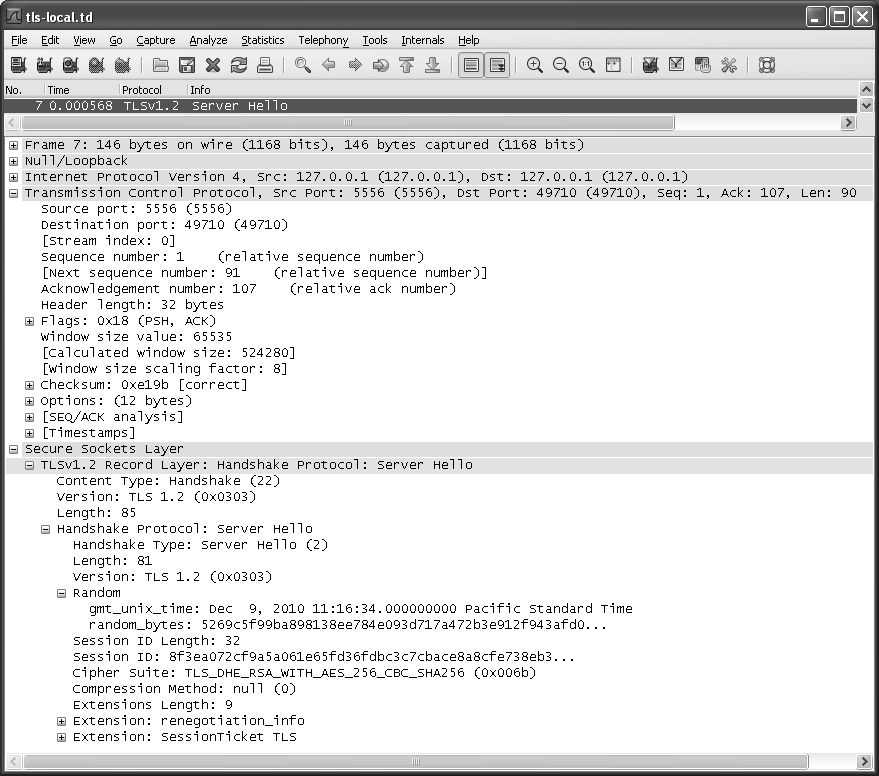
\includegraphics[width=0.7\textwidth]{imgs/18/18-33.png}
	\caption{TLS 1.2 中一个 ServerHello消息包含版本信息、所支持的密码套件与压缩算法以及一些扩
            展。此处,客户端支持 Diffie-Hellman 密钥协商。它使用AES-256算法用于加密,SHA-256
            算法用于完整性保护}
\end{figure}

由于 ClientKeyExchange 消息大多包含用于形成DH交换的二进制信息,所以不再对
其进行详细描述。下一条有趣的消息是报文段 13,它是一个包含 CertificateRequest 消息与
ServerHelloDone 消息的TCP 报文段。图18-35显示了它的内容。
图 18-35展示了一个包含 CertificateRequest 消息与 ServerHelloDone 消息的TCP报文
段。CertificateRequest 用于要求客户端提供证书,并使用后续的 CertificateVerify 消息认证它
的身份。应该使用RSA算法或来自测试CA证书颁发机构的DSS算法对要求的证书类型进
行签名。列出的签名算法包括 shal-rsa、shal-dsa、sha256-rsa、sha384-rsa 以及 sha512-rsa。
数据包15(未显示细节)所包含的证书消息拥有针对客户端与其公钥的证书链。在这种
情况下,主题字段包括“测试客户端”以及作为发布者的测试CA。因此客户端与服务器的
证书是被同一个CA签署的,而所谓的证书链只包含一个证书。对于客户端而言,如果要证
明自己拥有对应的私钥,它会生成一条 Certificate Verify 消息(数据包 19)。CertificateVerify
消息包含一个签名,它是通过客户端的私钥对迄今为止所有发送与接收的会话握手消息的散
列值进行签名。这样不仅能够证明客户端是真实的,还表示到目前为止客户端已经正确地参
与到TLS交换中,并没有丢失或重新排序任何消息。在 CertificateVerify 之后,更改密码消
息出现在随后的通信(已加密)中。

\begin{figure}[!htb]
    \centering
	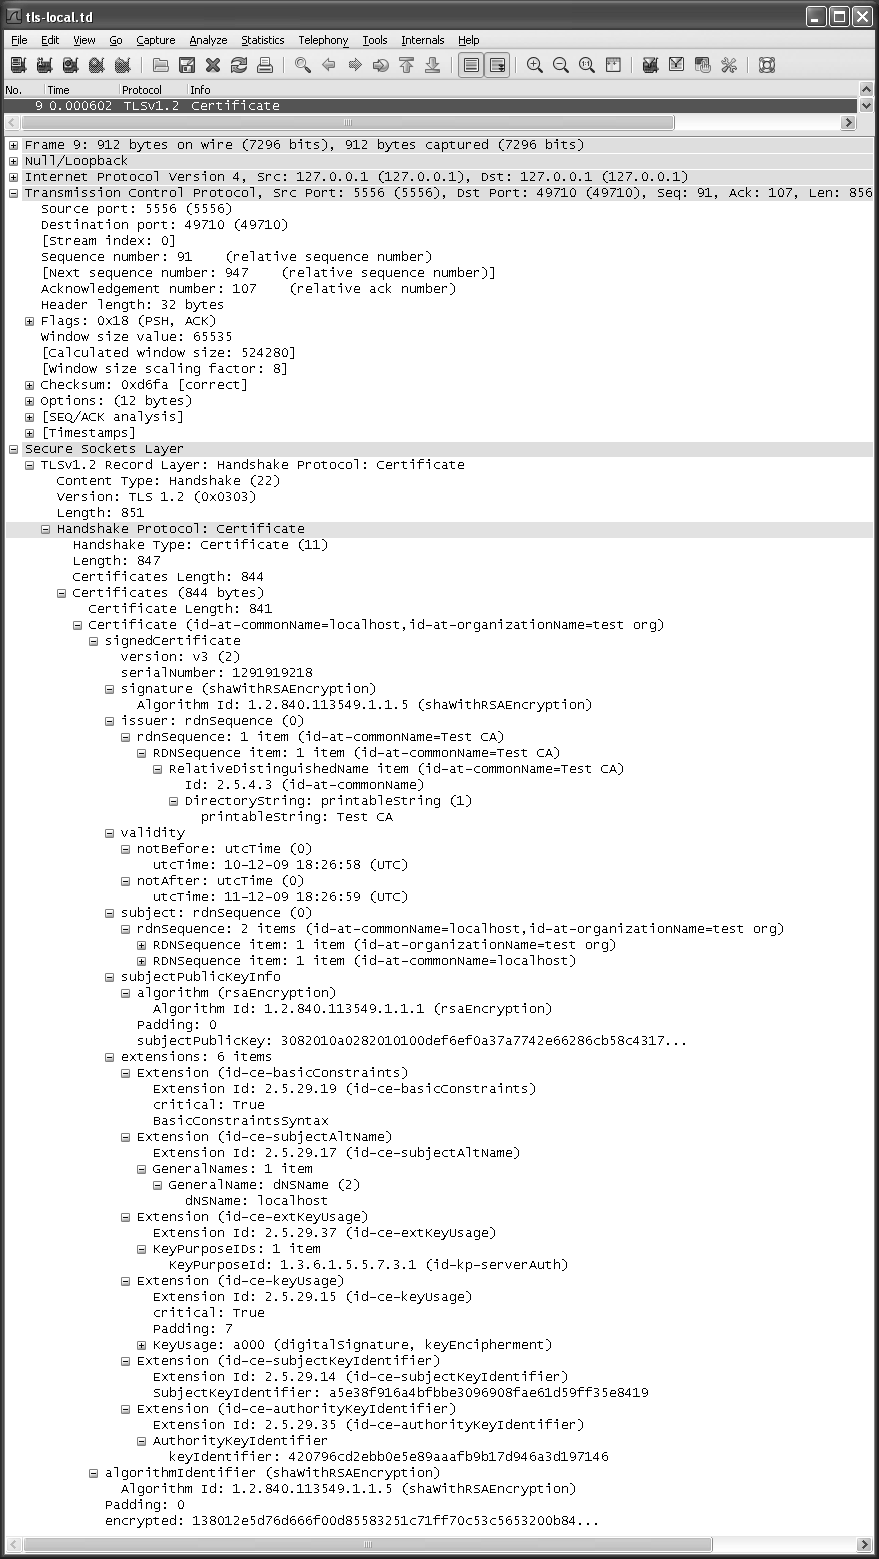
\includegraphics[width=0.7\textwidth]{imgs/18/18-34.png}
	\caption{服务器的 CertificateRequest 与 ServerHelloDone 消息都包含在相同的TCP 报文段中。客户端
            能够使用证书来认证服务器的身份。当服务器认证客户端的身份时也会使用相同的消息格式}
\end{figure}

\subsection{DTLS}
TLS 协议假设了一个基于流的底层传输协议来传输它的消息。数据报 TLS(DTLS)版
本放宽了这一假设,旨在使用与TLS 基本相同的消息格式但以其他方式达到相同的安全
目标。最初它是由那些诸如运行在UDP 协议上的SIP 协议引发的,但它不使用IPsec协议
\href{https://www.rfc-editor.org/rfc/rfc5406}{[RFC5406]}。DTLS 还可经过修改用于 DCCP \href{https://www.rfc-editor.org/rfc/rfc5238}{[RFC5238]}与 SCTP \href{https://www.rfc-editor.org/rfc/rfc6083}{[RFC6083]}。当前正在编写
的版本 DTLS1.0\href{https://www.rfc-editor.org/rfc/rfc4347}{[RFC4347]},基于 TLS 1.1。一个更新的基于TLS 1.2的版本正在制定中
[IDDTLS]。新版本还会使用图18-28所示的相同的协议分层,并采用绝大多数相同的消息交
换方式。

在缺乏可靠传输层的情况下提供类似TLS服务的主要挑战在于数据报可能会丢失、重
新排序或重复。这些问题会影响到加密与握手协议,这两者都依赖于 TLS协议。为了处理这
些问题,DTLS为记录层承载的每一条记录添加了一个明确的序列号(它们在普通TLS 中是
隐式的),并且借助(不同于)握手协议所使用的序列号制定出一个基于超时的重传方案。
\subsubsection{DTLS记录层}
在 TLS 中,由于计算一条记录的 MAC依赖于前一条记录,因此记录的顺序是非常重要
的。更特别的是,MAC 的计算依赖于每一条记录的隐式64位序列号。如果数据报乱序或丢
失,那么该序列号将会报错。为了补救这一问题,DTLS 在记录层使用明确的序列号。在每
一条 ChangeCipherSpec 消息发送之后,这些序列号被重置为数值0。它们也可以与一个附加
的16位历元数(epoch number)结合使用。历元数包含在每一条记录的头部。密码状态的每
一次变化都会使历元数加1。这样就解决了由于多个接近的握手产生多条包含相同序列号的
消息并出现传输冲突的问题。

DTLS 中的MAC 计算修改了对应的TLS版本,包含了一个由两个新字段(历元数在先,
后面是序列号)组成的64位块。这样就允许单独处理每一条记录。需要注意的是:在TLS
中一个错误的MAC会导致连接终止;而在DTLS中,终止一个完整的连接是没有必要的,
接收者会选择简单地丢弃包含错误 MAC的记录,或是发送一条警告消息(如果产生,必须
是终端)。

重复的消息会被简单地丢弃,或者被视为一个潜在的重放攻击。如果支持重放检测,那
么将会在接收端设置一个当前序列号窗口。要求该窗口至少容纳32条消息,但建议至少为
64条。这一方案与IPsec 中针对AH与ESP 的方案非常相似。如果到达记录的序列号小于窗
口左边沿对应的数值,那么会将它视为旧的或重复的记录而默默地丢弃。那些在窗口之内的
记录也会被检查,看是否出现重复。如果一条消息在窗口之内并且拥有正确的序列号,即便
出现顺序错乱的情况,也会将其保留下来。而那些拥有错误MAC的消息会被丢弃。那些拥
有正确 MAC却超出窗口右边沿的消息会使得右边沿增加。因此,右边沿代表已验证消息的
最高序列号。
一个数据报可能会包含多个 DTLS 记录,但是一条记录不可能跨越多个数据报。记录层
允许应用程序实现一个类似TCP的(参见第15章)PMTUD过程,并且在认可能被分片
时避免发送数据报。事实上,如果应用程序尝试发送的消息超过了PMTU或最大应用数据
报大小(PMTU 减去 DTLS 的负载),那么它应该收到一条错误提示。这条规则的一个例外是
DTLS在处理握手协议时,此时会包含比较大的消息。

\subsubsection{DTLS 握手协议}
握手协议的消息最大为224-1字节,但实际上大约为几千字节。这样就会超过典型的最
大UDP数据报大小的1.5KB。为了处理这一问题,握手协议的消息可能会通过分片过程跨
越多个 DTLS记录。每一个分片都包含在一条记录中,这些记录会包含在底层的数据报中。
为了实现分片,每一个握手消息都包含一个 16位的序列号字段、一个24位的分片偏移字段
以及一个24位的分片长度字段。

为了实现分片,原始消息的内容被分为多个连续的数据范围。每一个范围都要小于最大
分片大小,而且都包含在一个消息分片中。每一个分片都包含了与原始消息相同的序列号。
安全:可扩展身份认证协议、IP安全协议、传输层安全、DNS安全、域名密钥识别邮件635
分片偏移与分片长度字段都以字节表示。发送者会避免重叠数据范围,但接收者应具备处理
这一潜在问题的能力。因为发送者可能需要随时间推移而不断调整自己的记录大小,并且在
必要的时候进行重传。

为了处理消息丢失的问题,DTLS 具有简单的超时与重传功能。重传功能是以消息组的
形式运行的,也被称为“班次”。图18-36显示了完整的(左)与简化的(右)交换建立过程,
以及 DTLS 握手协议的状态机。

\begin{verbatim}
    完整交换
    客户端
    服务噐
    ClientHello
    (Session ID, CS, Comp)
    HelloVerifyRequest
    (Cookie)
    ClientHello
    (Cookie,.)
    ServerHello
    (Session ID, CS, Comp)
    Certificate(Server)
    ServerKeyExchange
    CertificateRequest
    ServerHelloDone
    Certificate (Client)
    ClientKeyExchange
    CertificateVerify
    -[ChangeCipherSpec]
    Finished
    -[ChangeCipherSpec]
    Finished
    3
    4
    简化交换
    (重新连接)
    客户端
    服务骼
    ClientHello
    (Session ID, CS, Comp)
    ServerHello
    (Session ID, CS, Comp)
    -[ChangeCipherSpec]
    Finished
    -[ChangeCipherSpec]
    Finished
    数据交换
    接收下一个
    班次
    各户端
    准备
    缓存
    班次
    发送
    接收RTX
    班次
    计时器
    超时
    没置RTX
    计时器
    等待
    发送上
    一个
    班次
    接收上一个
    班次
    发送或接收
    HelloRequest
    服务器
    启动
    结束
    图18-36
\end{verbatim}
在DTLS 中,必须处理丢失数据报的问题。初始的完整交换(左)包括6个班次的信息。每
个班次都能够重新传输。DTLS 简化交换(右上)只使用3个班次,并且与TLS 略不相同。
DTLS 在处理协议时保持一个3状态的有限状态机(右下)

在图 18-36中,班次号显示在完整交换与简化交换的中间区域。除了附加的HelloVerify
Request 与第2个 ClientHello 消息之外(现在包含cookie),完整交换与图18-30中完整的
TLS 交换非常类似。然而,简化的交换则不相同。在 DTLS 中由服务器发送第一条 Finished
消息,而在 TLS 中则是由客户端发送第一条 Finished 消息。
图18-36的右下部分描绘了在执行握手协议时 DTLS实现所使用的状态机。它包含3个
主要的状态:准备、发送与等待。客户端通过创建自己的 ClientHello 消息从准备状态启动。
服务器从等待状态启动,并且未缓存任何消息或启动重传计时器。在发送时,重传计时器会
被设置。在传输完成之后,协议会再次进人等待状态。如果重传(RTX)计时器超时,会使
协议重新回到发送状态来执行一次重传操作。当接收到来自对方的重传班次时也会出现同样
的状况。在后一种情况中,本地系统会以之前的传输部分丢失或完全丢失为理由而重传自己
的班次。这与端点重传所介绍的类似。如果一切顺利,一个班次在被接收后,本地系统结束
或返回到准备状态去形成下一个传输的班次。
状态机是由一个重传计时器驱动的,它的默认建议值1秒。如果在超时期限内接收
不到某一班次的响应,就会使用相同的握手协议序列号重新传输这一班次。然而需要注意的
是,记录层序列号仍然会向前增加。后续重传如果没有获得响应将会使 RTX的超时值加倍,
至少高达60s。在一次成功传输或一个长的空闲期之后,会重新设置该数值(10倍于当前计
时器的数值或更多)。

\subsubsection{DTLS DoS 保护}
当数据报用于替代可靠的字节流协议时,一些额外的安全考虑需要关注。特别值得关注
的是两个潜在的DoS攻击。攻击者在发送一个 ClientHello消息时伪造源IP 地址是很简单的
事情。许多这样的消息就会造成对DTLS服务器的DoS攻击,耗尽用于形成响应处理的资
源。该攻击的一个变种会包括多个拥有相同伪造IP 源地址的攻击主机。响应服务器会向这
些受害者的IP地址发送响应,这样这些受害主机就完成了对服务器的DoS 攻击。
包含于Hello交换中的一个无状态的cookie 验证过程能够帮助抵御 DoS攻击。当一台
服务器接收到一条 ClientHello 消息,它会生成一条新的包含32位 cookie(它可能是一个秘
密的函数、客户端的IP地址以及连接参数)的HelloVerifyRequest 消息。后续的 ClientHello
消息必须包含正确的 cookie,否则服务器会拒绝交换。这样服务器就能迅速摒弃那些未提供
正确 cookie的请求。这种方法并不能抵御来自多个合法IP 地址的协同攻击,因为这些IP地
址的主机都能够成功地完成cookie 交换。

\section{DNS 安全(DNSSEC)}
我们已经讨论了链路层、网络层与传输层流行的安全协议,本节我们开始讨论应用层。
虽然在作者撰写本书的时候还未广泛部署,但我们应该关注如何为域名系统(DNS)提供
增强的安全。DNS 安全不仅指 DNS中的数据(资源记录,RR)安全,还包含在同步或更
新 DNS服务器内容时的传输安全。鉴于 DNS 在 Internet 运行中的重要作用,针对其部署安
全机制会有深远的影响。这些机制称域名系统安全扩展(Domain Name System Security
Extensions,DNSSEC)。一系列 RFC 文档\href{https://www.rfc-editor.org/rfc/rfc4033}{[RFC4033]}\href{https://www.rfc-editor.org/rfc/rfc4034}{[RFC4034]}\href{https://www.rfc-editor.org/rfc/rfc4035}{[RFC4035]}对这些机制进行
了深人讨论。这些RFC文档有时被称为 DNSSECbis,这是因为它们取代了 DNSSEC早期的
规范文档。在我们进一步讨论 DNSSEC之前,先回顾一下 DNS 的基本描述(参见第11章)
是十分必要的。

安全:可扩展身份认证协议、IP安全协议、传输层安全、DNS 安全、域名密钥识别邮件 637
这些扩展提供了 DNS数据的源认证与完整性保护,以及(有限的)密钥分发设施。也
就是说,扩展提供了一种加密的安全方式来确定实体是否已对一块 DNS信息授权,以及接
收到的信息是否被篡改。DNSSEC还能够进行不存在性验证。DNS 响应能够指出某一受保
护的特定域名是不存在的并对此提供保护,就像保护那些指出某一个域名存在的响应一样。
DNSSEC 不能为DNS 信息提供保密性、DoS攻击保护以及访问控制。DNSSEC的传输安全性
是被单独定义的,我们将在讨论完 DNSSEC的核心数据安全功能之后对其进行简短的介绍。
DNSSEC是通过对“已知的”安全进行分层来调整解析器的。一个验证已知安全的解析
器(也称为验证解析器)会检查加密的签名,从而保证其处理的DNS数据是安全的。其他的
解析器,包括主机上的存根解析器以及递归域名服务器的“解析方”,可能已知安全但无法
进行密码验证。相反,这种解析器应当建立与验证解析器的安全关联。我们将关注验证解析
器,因为它们是最复杂、有趣的。在运行时,它们能够确定 DNS信息是否安全(所有的签
名都经检查有效)、不安全(签名有效地指出有些数据不应该存在,但却已经出现)、虚假(数
据出现在合理的位置,但是由于某些原因不能被验证)以及不确定(真实性无法得到验证,
通常是因为无法得到签名)。当没有其他可用信息时,不确定的情况是默认情况。
只有在域管理员签署了一个区域后 DNSSEC 才会安全地工作,它涉及一些信任基础,
服务器与解析器软件都参与其中。验证解析器会检查签名以保证 DNS信息是安全的,而且
它们必须配置一些初始信任锚点,这些锚点类似于PKI中的根证书。然而值得注意的是,
DNSSEC 不是一个 PKI,它只会提供有限的签名与密钥撒销功能。它不能够模拟证书撤销列
表\href{https://www.rfc-editor.org/rfc/rfc5011}{[RFC5011]}。

当执行一个带有 DNSSEC 的DNS查询时,一个已知安全的解析器就会使用DNS扩展
机制(EDNSO),并且将请求中一个 OPT元资源记录的DO 位置位(表示 DNSSEC OK)。该
位指出客户端不仅有兴趣而且有能力来处理与 DNSSEC相关的信息,并支持 EDNSO。DO
位在EDNSO元资源记录(参见\href{https://www.rfc-editor.org/rfc/rfc3225}{[RFC3225]}的第3节与\href{https://www.rfc-editor.org/rfc/rfc2671}{[RFC2671]}的第4节)的“扩展的
RCODE 与标志”部分,是其中第2个 16位字段的第1位。接收到那些DO 位未置位(或不
存在)请求时,会禁止服务器返回18.10.1节讨论的大多数资源记录,除非这些记录是在请
求中明确要求的。由于避免了承载那些与安全相关却又不被未知安全的解析器处理的资源记
录,所以这样做有助于提高 DNS的性能。由于 DNS通常会使用相对小的UDP数据包并且
常退回用TCP协议,而TCP 的3次握手就会增加对大响应的延迟,因此上述方法是十分有
益的。

当服务器处理来自一个 DNSSEC可用解析器的请求时,它会检查 DNS请求的CD
(Checking Disabled)位(参见第11章)。如果该位置位,那么表明客户端愿意接收包含未验
证数据的响应。在准备一个响应时,服务器通常会利用密码方法验证要返回的数据。成功的
验证结果会使得响应中的AD(Authentic Data,真实数据)位置位\href{https://www.rfc-editor.org/rfc/rfc4035}{[RFC4035]}。如果拥有一
条到达服务器的安全路径,那么一个安全已知但未验证的解析器在原则上是能够信任这条
信息的。然而,最好的情况是使用验证存根解析器——它能够进行加密验证,从而将查询的
CD 位置位。这样不仅提供了端到端的 DNS安全(即中间解析器不需要是可信的),还减少
了中间服务器的计算负担;否则,这些中间服务器不得不进行密码验证。

\subsection{DNSSEC资源记录}
如\href{https://www.rfc-editor.org/rfc/rfc4034}{[RFC4034]}所指定的,DNSSEC使用4个资源记录与两个消息头位(CD 与AD)。它
还需要支持EDNSO并且使用我们之前提到的DO位。在4个资源记录中,2个用于包含对
DNS域名空间的签名,另外2个用于帮助分发与验证密钥。\href{https://www.rfc-editor.org/rfc/rfc5155}{[RFC5155]}中有一处修改,新增
了2个资源记录,意在代替原始4个资源记录中的一个。

\subsubsection{DNS 安全(DNSKEY)资源记录}
首先,我们将查看 DNSSEC 是如何存储和分发密钥的。DNSSEC使用 DNSKEY 资源记
录来维护公钥。这些密钥只能与 DNSSEC一起使用;其他的资源记录(例如,\href{https://www.rfc-editor.org/rfc/rfc4398}{[RFC4398]}中
的证书资源记录 CERT RR)可能用于维护针对其他用途的密钥或证书。图18-37展示了一条
DNSKEY 资源记录中 RDATA 部分的格式。
0
15 16
31
标志
(16位)
协议
(8位)
算法
(8位)
图18-37
公钥
(长度可变)
DNSKEY资源记录的RDATA 部分包含一个只用于DNSSEC的公钥。标志字段包含了一
个区域密钥指示符(第7位)、一个安全入口点指示符(第15位)、一个撤销指示符(第8
位)。一般来说,区域密钥位是为所有的 DNSSEC密钥设置的。如果公开的SEP位也被置
位,那么该密钥通常被称为密钥签名密钥,并用于验证对子区域的授权。如果没有置位,该
密钥通常是一个区域签名密钥,拥有更短的验证周期,通常用于签名区域的内容但不授权。
DNSKEY 资源记录所包含的密钥会与其算法字段指定的算法一同使用
图18-37中的标志字段目前定义了3位。第7位是区域密钥位字段。如果置位,那么
DNSKEY 资源记录拥有者的名称必须为区域的名称,并且所包含的密钥也被称为区域签名
密钥(Zone Signing Key,ZSK)或密钥签名密钥(Key Signing Key,KSK)。如果没有置位,
那么记录将会维护另一种不能用于验证区域签名的DNS密钥。第15位称安全入口点
(SEP)位。它作为调试或签名软件时的一条提示,能够根据密钥的用途做出明智的猜测。签
名验证不会解释SEP位,但该位置位的密钥通常为KSK,并通过验证子区域的密钥来确保
DNS层次结构的安全(借助DS记录,参见18.10.1.2节)。第8位是撤销位\href{https://www.rfc-editor.org/rfc/rfc5011}{[RFC5011]}。如
果该位置位,则表示密钥不能用于验证。协议字段维护的数3用于这一版本的 DNSSEC。
算法字段指出了签名算法 [DNSSECALG]。根据\href{https://www.rfc-editor.org/rfc/rfc4034}{[RFC4034]},只有DSA 与具有 SHA-1 的 RSA
(数值分别为3和5)才被定义用于 DNSKEY 资源记录,但是其他的规范能够支持其他算法
(例如,针对ECC-GOST 的\href{https://www.rfc-editor.org/rfc/rfc5933}{[RFC5933]}(数值为12),针对 SHA-256 的\href{https://www.rfc-editor.org/rfc/rfc5702}{[RFC5702]}(数值为8))。
这些数值还可以与其他若干 DNSSEC资源
0
15 16
31
记录一起使用。公钥字段维护了一个公钥,
密钥标签
(16位)
摘要类型
(8位)
它的格式依赖于算法字段。
18.10.1.2 授权签名者资源记录
授权签名者(DS)资源记录用于指定
一条 DNSKEY 资源记录,通常从一个父区
域到一个子区域。这些记录在授权过程中
用来验证公钥(参见18.10.2节)。DS资源
记录的格式如图18-38所示。
算法
(8位)
摘要
(长度可变)
图18-38
DS 资源记录的RDATA 部分在密钥标签
字段包含了对一条 DNSKEY 资源记录的
非唯一参考,还包含了对 DNSKEY 资源
记录及其所有者的消息摘要。此外,还有
对摘要类型与算法的说明
安全:可扩展身份认证协议、IP安全协议、传输层安全、DNS 安全,域名密钥识别邮件
639
图18-38中的密钥标签字段是一条 DNSKEY 资源记录的参考,但它不是唯一的。多条
DNSKEY 资源记录可能会拥有相同的标签值,因此该字段只能作为查找的提示(确认验证仍
然是必要的)。该字段的数值是作为16位的未签名数据之和来计算的,其中包含了图18-37
中所示的 DNSKEY 资源记录的RDATA 部分(负载被忽略)。算法字段使用了与 DNSKEY
资源记录的算法字段相同的数值。摘要类型字段指出了所用的签名类型。\href{https://www.rfc-editor.org/rfc/rfc4034}{[RFC4034]}中只定
义了数值1(SHA-1),而SHA-256(数值2)是通过\href{https://www.rfc-editor.org/rfc/rfc4509}{[RFC4509]}指定的。当前的列表包含在
DS 资源记录类型摘要算法注册表中[DSRRTYPES]。摘要字段包含了将要引用的 DNSKEY
资源记录的摘要。具体地说,该摘要的计算方法如下:
摘要=摘要算法(DNSKEY 所有者名|DNSKEY RDATA)
此处|是连接运算符,而DNSKEY RDATA 的数值是根据引用的DNSKEY 资源记录来计算
的。它的计算方法如下:
DNSKEY RDATA=标志| 协议 | 算法 | 公钥
在SHA-1 的情况下,摘要的长度为20字节,而在SHA-256 的情况下,长度32字
节。DS资源记录用于在跨越区域边界的认证链中提供一个下行链路,所以引用的DNSKEY
资源记录必须是一个区域密钥(即,在 DNSKEY 资源记录中标识符字段的第7位必须置位)。
注意在作者撰写本书时,一个称为DS2的DS资源记录的变种正在商定中
[IDDS2]。它在DS资源记录中引入了一个典型签名者名称,这样拥有相同内容的
多个区域可以被命名为不同的名称,并被多个签名者签署。此外,还有一个 DLV
资源记录[RFC44311用于提供授权,以免一个父区域未被签名或未被 DS 资源记录
发布。DLV 资源记录的格式与 DS资源记录相同,只是解释不同。
18.10.1.3 下一步安全(NSEC 和 NSEC3)资源记录
我们已经看到,除了维护资源记录之外还要保障相关密钥的安全,本节我们将继续讨论
验证区域结构的记录与其所包含的资源记录。下一步安全(NextSECure)资源记录(NSEC)
用于在规范有序的名称(参见18.10.2.1 节)或一个NS类型的RRset(资源记录集)授权点中
维护“下一个”RRset所有者的域名(回忆一下,一个 RRset 是一组具有相同所有者、类、
TTL 或类型但拥有不同数据的资源记录)。
它还维护位于 NSEC资源记录的所有者名
0
31
称中的RR类型列表。这样能够为区域结
构提供认证与完整性验证。NSEC资源记
录的格式如图 18-39所示。
NSEC 资源记录用于在一个区域中形
成一条与资源记录集(RRset)相关的链。
因此,一个不在链上的 RRset 会被显示
不存在。这种方法提供了前文提到的可认
15 16
下一个域名
(长度可变)
类型位图
(长度可变)
图 18-39
NSEC 资源记录的RDATA 部分包含了下
一个 RRset 所有者在规范有序的区域中的
名称。它也指出了哪一种 RR类型出现在
NSEC资源记录所有者的域名中
证的拒绝存在特性。下一个域名字段维护
一个区域的规范有序的域名链中的下一个条目,并且没有使用第11章介绍的域名压缩技术。
链中最后一条 NSEC记录在这一字段的数值区域顶点(区域的SOA 资源记录的所有者
名称)。
NSEC资源记录的类型位图字段维护了一张关于 RR类型的位图。这些RR类型记录在
NSEC资源记录所有者的域名中。最多有64K个可能的类型,其中大约有100种限定了日期
[DNSPARAMS]。只有一小部分被广泛使用。例如,Internet 的根区域(域名为“”),它与
DNSSEC一起从2010年7月15日开始工作,包含了ac(一个国家及地区代码顶级域名)的
下一个域名字段与一张指出当前记录类型(包括NS、SOA、RRSIG、NSEC 以及 DNSKEY)
的位图。

为了对存在的类型进行编码,整个资源记录类型的空间被划分为256个“窗口块”,编
号从0到255。对于每一块的序号而言,用1位掩码最多能够对256个资源记录类型进行编
码。假设一个块的编号为 N并且位位置P,那么相关的资源记录类型编号为(N*256+ P)。
例如,在块1中,与资源记录类型258(目前尚未定义的一种类型)相关的位位置是2。编码
的字段如下:

类型位图=(窗口块号 | 位图长度|位图)

其中,|为连接运算符,而*代表克林(Kleene)闭包(即,0个或多个)。窗口块号的每一个
实例都包含了一个0~255的数值,位图长度包含了对应位图的字节长度(最大值为32)。
窗口块号与位图长度均为一个字节,而位图可以到32字节(256位,每一位对应窗口中可能
的资源记录类型)。不存在资源记录类型的块是不包含在内的。针对那些跨越多个块并且稀
疏出现的类型,已对编码进行了优化。例如,如果只有资源记录类型1(A)与15(MX)出现,
该字段的编码如下:

0x00024001=(0x000x02|0x4001)

定义在\href{https://www.rfc-editor.org/rfc/rfc4034}{[RFC4034]}中的NSEC记录的原始结构造成了这样一种情况:任何人都能通过
遍历 NSEC链而列举出一个区域中的权威记录。这种情况称为区域列举。这在许多部署中
是一种不希望有的信息“泄露”机会。因此
0
15 16
31
[RFCS155]定义了一对资源记录,意在取代
NSEC。第一条记录称为 NSEC3,它使用资
源记录所有者域名的加密散列值来取代未编
散列算法
(8位)
混淆值长度
(8位)
标志
(8位)
迭代次数
(16位)
码的域名。图18-40显示了它的格式。
混淆值
(长度可变)
在NSEC3记录中,散列算法字段标识
了应用于下一个所有者名称的散列函数,以
散列长度
(8位)
产生下一个散列的所有者字段。只有 SHA-1
下一个散列所有者
(长度可变)
(数值 1)限定了日期[NSEC3PARAMS】。
标志字段的低比特位包含了一个 opt-out 标
志。如果置位,它将指出 NSEC3记录可能
包含未签名的授权。它用于对一个没有被要
求或不希望被签名的子区域授权(NS RRset)
的情况。迭代次数字段指出散列函数使用了
多少次。较大的迭代次数有助于防止找到与
NSEC3 记录中的散列数值相关的所有者名
称(宇典攻击)。混淆值长度字段给出了混
淆值字段的字节长度。混淆值字段包含了一
个在计算散列函数之前附加于原所有者名称
的数值。它的目的在于帮助抵御字典攻击。
类型位图
(长度可变)
图18-40
NSEC3 资源记录的 RDATA 部分包含了
下一个 RRset 所有者在规范有序区域中
的名称的散列值。迭代次数字段指出了
散列函数使用的次数。在使用散列函数
之前,长度可变的混淆值(Salt,“盐”)
被附加到名称上,以抵御字典攻击。类
型位图字段使用与 NSEC RR 相同的结
构。NSEC3PARAM 记录非常相似,但
只包含散列参数(不是下一个散列所有
者或类型位图字段)
安全:可扩展身份认证协议、IP安全协议、传输层安全、DNS 安全、域名密钥识别邮件 641

\href{https://www.rfc-editor.org/rfc/rfc5155}{[RFC5155]} 指出的第2条资源记录被称为 NSEC3PARAM 资源记录(未单独显示)。除
了不包含散列长度、下一个散列的所有者以及类型位图字段外,它使用与NSEC3资源记录
相同的格式。权威的名称服务器在为否定的响应选择NSEC3记录时使用 NSEC3PARAM资
源记录。NSEC3PARAM 资源记录为计算一个散列所有者名称提供了所需的参数。
为了获得下一个散列所有者字段的散列值,需要进行以下计算:
IH(0) =H(所有者名称 | 混淆值)
IH(k)=H(IH(k-1) |混淆值),若k>0
下一个散列所有者=H(IH(迭代次数)|混淆值)
其中H是散列算法字段指定的散列函数,所有者名称必须按照标准的格式。迭代次数与混淆
值取自 NSEC3资源记录的相关字段。
为了避免混淆 NSEC与NSEC3 资源记录类型,\href{https://www.rfc-editor.org/rfc/rfc5155}{[RFC5155]} 在 NSEC3 资源记录的区域中
分配并要求使用特殊的安全算法编号6和7,作为标识符3(DSA)和5(SHA-1)的别名。
不知道 NSEC3记录类型的解析器在接收到这些数值后会将它们作为不安全的记录处理。这
样就提供了一种有限的向后兼容能力(即失败,但这样做并没有错误地解释资源记录数据)。
18.10.1.4 资源记录签名资源记录
从DNS的结构到它的内容,我们需要一种方法为资源记录提供源认证与完整性保护。
DNSSEC 使用名为资源记录签名(Resource
0
15 16
31
Record Signature,RRSIG)的资源记录来
签署并验证 RRset 中的签名。区域中每一
覆盖类型
(16位)
算法
(8位)
标签
(8位)
条授权的资源记录都必须签名(父区域中出
现的粘贴记录与授权 NS记录不需要签名)。
一条RRSIG 资源记录包含了某一特定
RRset 的数字签名,以及使用哪一个公钥来
源TTL
(32位)
签名到期
(32位)
签名成立
(32位)
验证签名的信息,如图18-41 所示。
覆盖类型字段指出了签名适用的 RRset
密钥标签
(16位)
签名者名称
(长度可变)
类型。它的数值来自标准的RR类型集合
[DNSPARAMS]。算法字段指出了签名算
签名
(长度可变)
法。根据\href{https://www.rfc-editor.org/rfc/rfc4034}{[RFC4034]},只有DSA与带有
SHA-1的RSA(数值分别为3与5)才能
图18-41
RRSIG 资源记录的 RDATA 部分包含了一
用于 RRSIG 资源记录,但是\href{https://www.rfc-editor.org/rfc/rfc5702}{[RFC5702]}涵
个 RRset 的签名。RRset 出现在授权域中
盖了SHA-2算法,而\href{https://www.rfc-editor.org/rfc/rfc5933}{[RFC5933]}涵盖了
的TTL 也包含在内。此外,还指出了算
GOST 算法(来自于俄罗斯)。标签字段给
法与签名的有效期。密钥标签字段指出那
出了在 RRSIG 资源记录的原所有者名称中
些包含公钥的 DNSKEY 资源记录(该公
的标签数目。原TTL 字段维护了一份 TTL
钥用于验证签名)。标签字段指出有多少
副本,这份副本是当RRset 出现于授权区
标签构成了资源记录的原所有者名称
域时保留下来的(缓存名称服务器能够减少 TTL)。签名到期与签名成立字段指出了一个签
名有效期的开始与结束时间,从世界协调时间(UTC)的1970年1月1日0点0分0秒开始
以秒为单位显示。密钥标签字段标识那些用于获得某种特殊公钥的 DNSKEY 资源记录。这
种公钥对于验证签名字段所包含的签名而言是必需的。密钥标签字段将使用之前DS资源记
录所使用的格式。

\subsection{DNSSEC运行}
现在我们已经讨论了 DNSSEC需要的所有资源记录,知道如何使用面向安全区域的
DNSSEC。如前文所述,在定义 NSEC与NSEC3的记录类型时,首先需要一个规范有序的
定义。针对某一区域定义规范顺序的目的是为了以一种能够被签名的可重现方式来列举区域
的内容(好的散列函数会根据同一内容的不同顺序产生出不同的数值)。

\subsubsection{规范顺序与形式}
有3种规范顺序引起我们重视:一个区域中规范的名称顺序,一条资源记录中规范的形
式,以及一个 RRset 中的规范顺序\href{https://www.rfc-editor.org/rfc/rfc4034}{[RFC4034]}。在第11章已经介绍过,每一条资源记录都
有一个包含多个标签的所有者名称(所有者域名)。通过将名称中的每一个标签作为左对齐
的字符串,同时将大写的US-ASCII 字母作为小写字母,我们能够形成一个名称列表。首先
通过它们最重要(最右边)的标签进行排序,然后根据次重要的标签排序,依次类推。在一
个0值字节之前将缺省一个字节。一个正确的规范顺序将会使用com,例如company.com、
*.company.com、UK.company.COM、usa.company.com 等。此外,还可以使用通配符。
对于一个特的资源记录而言,需要有一个定义良好的规范形式。这一形式要求资源记
录遵循以下规则:

1. 每一个域名都是一个完全限定域名并被完全展开(无压缩标签)。
2. 在所有者名称中的所有大写的US-ASCII 码字符都需要被它们的小写版本代替。
3. 对于任何类型号为2~9、12、14、15、17、18、21、24、26、33、35、36、39以
及38的记录,在它们的RDATA 部分出现的域名中,所有大写的US-ASCII 码字符都需要被
它们的小写版本代替。
4. 任何通配符都不会被取代。
5. 当出现在原权威区域或覆盖 RRSIG 资源记录的原TTL字段,TTL 将会设置为原始
数值。

注意 一些说明与重要修改目前正应用于 DNSSECbis 族的基本文件中。读者可以
查阅最新版本的[IDDCIN]来获得具体的细节。

一个 RRset 中的资源记录的规范顺序遵循与所有者名称相同的规则,只不过所有者名称
以规范形式应用于资源记录的 RDATA 内容,就像对待左对齐的字节串那样。

\subsubsection{签署区域与区域削减}
DNSSEC依赖于签名区域。这样的区域包括 RRSIG、DNSKEY 以及 NSEC(或NSEC3)
资源记录,而且如果有一个签名授权点,它可能还会包含 DS资源记录。签名使用公钥加密,
公钥的存储与分发通过DNS来完成。图18-42展示了位于父子区域之间的抽象授权点。
在图18-42 中,父区域包含了自己的 DNSKEY 资源记录,它能够提供与使用 RRSIG资
源记录(可能出现多个 DNSKEY)来签名一个区域中的所有授权 RRset 的私钥相关的公钥。
父区域中的一条 DS资源记录提供子顶点的一条 DNSKEY 资源记录的散列值。这样就建立
起一条从父区域到子区域的信任链。一个信任父区域的DS资源记录的验证解析器也能验证
子区域的DNSKEY 资源记录,以及最终的 RRSIG 和子区域中签名的RRset。这种情况只会
在验证者拥有一个与父区域 DSNKEY 资源记录相连的信任根节点时才会发生。
安全:可扩展身份认证协议、IP 安全协议、传輸层安全、DNS安全、域名密钥识别邮件
: 643
签名
RRSIG资源记录
(用于DNSKEY RRset)
DNSKEY资源记录
(在父区域)
RRSIG资源记录
(用于DS RRset)
验证
RRSIG资源记录
(用于NSEC RRset)
签名
签名
NSEC资源记录
(位于顶点的类型)
DS资源记录
(子区域的DNSKEY
资源记录的散列值)
示例
父区域
授权点
(父区域名称)
(同一所有者)
散列
区域划分
区域顶点
(子区域名称)
DNSKEY资源记录
(位于顶点)
签名
RRSIG资源记录
(用于DNSKEY)
子示例
子区域
NSEC资源记录
(SOA类型位置位)
签名
RRSIG资源记录
(用于NSEC)
NS资源记录
(位于顶点)
签名
RRSIG资源记录
(用于NS)
图18-42 对一个已认证授权的区域的区域划分包括父区域的一条DS 资源(父区域包含了子区域
DNSKEY 资源记录的散列值)。所有的 RRset 都使用相关的RRSIG 资源记录进行签名,除
了父区域的授权NS资源记录(与粘贴记录)。NSEC资源记录能用于验证区域中的类型,并
包含一个 SOA 资源记录类型来指出子区域的顶部
\subsubsection{解析器操作示例}
给定一条关于签名区域的链与一个安全已知的验证解析器,我们能看到一个 DNS响
应的内容是如何验证的。在最好的情况下,能够通过一条信任链从根区域到达一个区域。
ICANN通过根区域中的DS记录与已签名的 DNSKEY 资源记录[TLD-REPORT]来维护一个
DNSSEC 已启用的区域列表。
假设我们希望为域名www.icann.org 处理并验证一个A 资源记录类型。从根区域出发向
下,我们首先需要根的信任锚点(即 DNSKEY资源记录)、包含于根名称服务器中的org.的
DS记录,还可能需要 RRSIG 与 NSEC(NSEC3)记录。然后,我们利用域名 org.与 icann.
org.以及相关的 DNS服务器重复这一过程。我们开始于根区域:
\begin{verbatim}
    Linux8 dig ea.root-servers.net.•dnskey +noquestion +nocoments\
    ;; Truncated,retrying in rCP mode.
    ; <<>> DiG 9.7.2-P3 <<>> ea.root-servers.net.•dnskey
    +noquestion +nocomments +nostats +multiline
    ;(1 server found)
    iiglobal options:
    8( AWEAAagAIK1 ••);key
    id=
    19036
    903
    904
    905
    644
    第18章
    86400
    86400
    IN
    IN
    DNSKEY
    DNSKEY
    256
    8(AWEAAb5gVAz •.);key id = 21639
    8( AWEAACAPhPM
    ; key id = 40288
\end{verbatim}
此处我们看到根区域的信任锚点,它构成 Internet 中所有 DNSSEC信任关系的根部。第
一个密钥是 KSK,由数值257指出(SEP位为1),它是用于构成信任链的主要成员之一。
其他的密钥被标记为ZSK。接下来,我们希望看到的所有记录都应该是存在的并且拥有合适
的签名。根证书中有趣的 RRSIG 记录如下所示:
\begin{verbatim}
    Linux8 dig @a.root-servers.net.• rrsig +noquestion +nocomments\
    +nostats +noauthority +noadditional
    ii Truncated,retrying in rCP mode.
    ;<<>> DiG 9.7.2-P3 <<>> ea.root-servers.net.• rrsig +noquestion
    +nocomments +nostats
    +noauthority +noadditional
    ;(1 server found)
    ii global options: +cmd
    • 86400 IN
    RRSIG NSEC 80 86400 20101228000000 20101220230000
    40288•RyoGBldxxX..
    RRSIG DNSKEY
    8 0 86400 20110105235959 20101221000000
    19036• f8bzNvPmHR.•.
\end{verbatim}
包含 DNSKEY 记录的 RRSIG 使用密钥标签19036,它与根区域的 DNSKEY 资源记录
所包含的KSK 相匹配。根区域包含了其他 RRSIG 记录(用于它的SOA与NS记录),但我
们更关心的是用于 DNSKEY 与NSEC 资源记录的 RRSIG。只要额外地确保 DNSKEY 资源
记录存在,我们就能够检查根的NSEC资源记录,从而验证它的类型是否存在。
\begin{verbatim}
    Linux& dig @a.root-servers.net. • nsec +noquestion +nocomments\
    +nostats +noauthority +noadditional
    ;<<>> DiG 9.7.2-P3 <<>> @a.root-servers.net.• nsec +noquestion
    +nocomments +nostats +noauthority +noadditional
    ; (1 server found)
    ii global options:+cmd
    86400 IN
    NSEC ac.NS SOA RRSIG NSEC DNSKEY
\end{verbatim}
这就确认了根区域正式包括的RRset类型包括:NS、SOA、RRSIG、NSEC 以及
DNSKEY,因此我们到目前为止都处于良好的状态(还要注意的是,ac.是根区域的规范顺序
中的第一个TLD)。接下来,我们需要检查从根到域名 org.授权的签名。可以按照下述过程
操作:
\begin{verbatim}
    Linux8 dig @a.root-servers.net. org. rrsig +noquestion +nocomments\
    +nostats +noadditional +dnssec
    ;<<>> DiG 9.7.2-P3 <<>> @a.root-servers.net. org. rrsig +noquestion
    +nocomments +nostats +noadditional +dnssec
    ;(1 server found)
    i;global options: +cmd
    org• 172800
    IN
    do.org.afilias-nst.org.
    org. 172800
    IN
    b2.org.afilias-nst.org.
    org. 172800
    IN
    org. 172800
    a0.org.afilias-nst.info.
    • IN
    bo.org•afilias-nst.org•
    org. 172800
    IN
    a2.org.afilias-nst.info.
    org•172800
    IN
    co.org.afilias-nst.info.
    org. 86400
    IN.
    21366 7 2 96EEB2FFD9 •••
    org. 86400
    IN
    21366 7 1 E6C1716CFB
    org• 86400 IN
    RRSIG
    86400 20101228000000 20101220230000
    • jpcJOGclvvlnx9Kvz5
\end{verbatim}
DS RRset 的存在以及它相关的 RRSIG 表明确实有一个 DNSSEC安全授权。RRSIG资
安全:可扩展身份认证协议、IP安全协议、传输层安全、DNS 安全、域名密钥识别邮件645
源记录包含密钥标签 40288,它指出了我们之前在根区域(ZSK)看到的第三个 DNSKEY资
源记录。在查询中NS记录为我们提供了下一步需要使用的服务器名称。通过重复在根区域
做出的查询,我们可以继续下去,但这一次使用org.。我们在一台NS资源记录指出的服务
器中为根区域的org.进行这些查询。
\begin{verbatim}
    Linux8 dig edo.org.afilias-nst.org.org.dnskey +dnssec +nostats\
    +noquestion +multiline
    ; <<>> DiG 9.7.2-P3 <<>> edo.org.afilias-nst.org.org•dnskey +dnssec
    +noquestion tmultiline
    ;(1 server found)
    i;global options:
    i; Got answer:
    >>HEADER<- opcode:QUERY,status:NOERROR,id:8061
    ;;flags:gr aa rd; QUERY:1,ANSWER:6,AUTHORITY:0,ADDITIONAL: 1
    ;;WARNING:recursion requested but not available
    ii OPT PSEUDOSECTION:
    ;EDNS:version: 0,Elags:do: udp: 4096
    ;; ANSWER SECTION:
    org.
    900
    DNSKEY
    256 3 7 (AWEAAZTErUF •);key id = 1743
    Org•
    900 IN
    DNSKEY
    256 3 7( AWEAAazTpnm••.
    );key id = 43172
    Org.
    900
    IN
    DNSKEY
    257
    3 7 ( AWEAAYpYfj3 •);key id = 21366
    org.
    900
    IN
    •DNSKEY
    257 3 7(AWEAAZTjbIO •);key id = 9795
    Org•
    900 IN
    RRSIG DNSKEY 7 1 900 20101231154644
    20101217144644 21366 org.
    aIZgEsoJO+08ZXM
    org•
    900 IN
    RRSIG DNSKEY 71 900 20101231154644
    20101217144644 43172 Org•MWWOsWBdEmM8CiM••
\end{verbatim}
此处我们看到有4个 DNSKEY 资源记录,其中两个为KSK(数值为257),而另外两个
为ZSK(数值256)。列出的第三个 DNSKEY 资源记录(21366)与我们在根区域中发现
的DS资源记录相关。RRSIG 资源记录使用这一密钥,再加上ID 为43172的ZSK。为了验
证它们存在的合法性,可以查看也许 org. 中存在的 NSEC或 NSEC3 记录:
\begin{verbatim}
    Linux&
    dig edo.org.afilias-nst.org. org. nsec +dnssec +nostats\
    +noquestion
    ; <<>> DiG 9.7.2-P3 <<>> edo.org.afilias-nst.org. nsec org. +dnssec
    +nostats +noguestion
    ; (1 server found)
    ii global options:
    +cmd
    i; Got answer:
    ii->>HEADER<<- opcode: QUERY,
    status:NOERROR,id:61632
    i; flags:qr aa rd; QUERY:1,ANSWER: 0,AUTHORITY:4,ADDITIONAL:1
    ;;WARNING:recursion requested but not available
    ii OPT PSEUDOSECTION:
    ;EDNS:version:0,flags: do; udp: 4096
    ;;AUTHORITY SECTION:
    h9p7u7tr2u91dov01js911gidnp9ou3h.org. 86400 IN NSEC3 1 1 1
    D399EAAB
    H9RSFB7FPF2L8HG35CMPC765TDK23RP6
    NS SOA RRSIG DNSKEY NSEC3PARAM
    h9p7u7tr2u91d0v0ljs911gidnp90u3h.org.
    86400 IN RRSIG NSEC3 7 2
    86400 20110105003654
    20101221233654
    43172 org.eBtna4fok
    •••
\end{verbatim}
此处,可以看到一条带有所有者名称的NSEC3记录等同于 org.的散列版本。它指出存
在一条 DNSKEY与一条 RRSIG 记录,以及NS与NSEC3PARAM 记录。根据最后一个类
型,我们能够判断 NSEC3的信息。
\begin{verbatim}
    Linux&•ldig Cao.org.afilias-nst.info.org. nsec3param +dnssec\
    +nostats +noadditional +noauthority +noquestion
    ; <<>> DiG 9.7.2-P3 <<>> ea0.org.afilias-nst.info.org.nsec3param
    +dnssec tnostats +noadditional +noauthority +noquestion
    ;(1 server found)
    iiglobal options: +cmd
    ;; Got answer:
    ;->>HEADER<<- opcode:QUERY,status:NOERROR,id: 38602
    ii Flags: qr aa rd: QUBRY:1,ANSWBR: 2, AUTHORITY: 7,ADDITIONAL: 13
    ;;WARNING:recursion requested but not available
    i; OPT PSEUDOSECTION:
    ;EDNS:version:0,flags:do; udp: 4096
    i; ANSWER SECTION:
    org•
    Org•
    900
    900
    IN
    IN
    NSEC3PARAM 1 0 1 D399EAAB
    RRSIG NSEC3PARAM 7 1 900 20101231154644
    20101217144644 43172 org.ES2kFw53elY ...
\end{verbatim}
可以看到(签名)数值D399EAAB是匹配的,因此NSEC3PARAM 的资源记录是与
NSEC3资源记录匹配的。我们还发现 RRSIG 资源记录中的签名来自与DNSKEY(ID为
43172)相关的私钥。如果所有的签名都匹配,那么至此我们已得到一个正确的信任链。为
了完成这一条链,我们还需要 icann.org 的信息:
\begin{verbatim}
    Linux8 dig @ao.org.afilias-nst.info.icann.org. any +dnssec +nostats\
    +noadditional
    ;<<>> DiG 9.7.2-P3 <<>> @a0.org.afilias-nst.info.icann.org. any
    tdnssec +nostats +noadditional
    ;(1 server found)
    :;global options:tcmd
    ;;Got answer:
    ii >HEADER- opcode:QUERY,status:NOERROR,id:61234
    i;flags:ar rd; QUERY:1,ANSWER:0,AUTHORITY:8,ADDITIONAL:3
    ;;WARNING: recursion requested but not available
    ;;OPT
    PSEUDOSECTION:
    ;EDNS: version: 0,flags:;udp: 4096
    i; QUESTION
    SECTION:
    ;icann.org•
    IN
    ANY
    i; AUTHORITY SECTION:
    icann.org.
    86400 IN
    icann.org.
    86400 IN
    icann.org
    86400 IN
    icann.org•
    86400 IN
    icann.org•
    86400 IN
    icann.org•
    86400 IN
    icann.org•
    86400 IN
    icann.org•
    86400 IN
    NS
    a.iana-servers.net.
    NS
    b.iana-servers.org•
    NS
    c.iana-servers.net.
    NS
    d.iana-servers.net.
    NS
    ns.icann.org•
    DS
    41643 7 1 93358DB•
    DS
    41643 7 2 B8AB67D
    RRSIG DS 72 86400 20101231154644
    20101217144644 43172 org.CZ1230w/1 ...
\end{verbatim}
可以看到DS资源记录指出对icann.org.已签名的授权。针对DS RRset 的 RRSIG 是在
ID 43172 的ZSK 的基础上签署的。通过NS记录中的一台服务器,我们能够查看最终的
服务器:
\begin{verbatim}
    Linux8 dig ea.iana-servers.net. icann.org.dnskey +dnssec +nostats\
    +noquestion +multiline
    ; <<>> DiG 9.7.2-P3 <<>> ea.iana-servers.net.icann.org.dnskey +dnssec
    安全:可扩展身份认证协议、IP安全协议、传輸层安全、DNS 安全、域名密钥识别邮件647
    tnostats +noquestion +multiline
    ;(1 server found)
    i;global options: +cmd
    ;; Got answer:
    i;->>HBADER<<- opcode:QUERY,status:NOERROR,id:22065
    ii flags:gr aa rd; QUERY:1,ANSWER:5,AUTHORITY:0,ADDITIONAL:1
    ;;WARNING:recursion requested but not available
    :; OPT PSEUDOSECTION:
    ;EDNS:version:0,flags:i udp:4096
    i; ANSWER SECTION:
    icann.org. 3600 IN
    DNSKEY 256 3 7
    (AWEAAbDmrVc ••);key id = 41295
    icann.org. 3600 IN
    DNSKEY 256 3
    7(AWEAAbgrrzd ••);key id = 55469
    icann.org. 3600 IN
    DNSKEY 257 3 7(AWEAAZuSdr4 •);key id = 7455
    icann.org. 3600 IN
    DNSKEY 257 3 7(AWEAACYgUBH
    icann.org•3600 IN
    RRSIG DNEKEY 7 2 3600 20101229153632
    •);key id = 41643
    20101222042536 41643 icann.org.
    UxR/5vyOIS
\end{verbatim}
此处可以看到存在4个 DNSKEY 资源记录,其中两个为KSK,而另外两个为ZSK。列
出的第4个 DNSKEY 资源记录与 org.区域的DS资源记录相关。RRSIG 资源记录使用这一
密钥。为了找到最终查询的答案,我们请求了记录A:
\begin{verbatim}
    Linux8 dig ea.iana-servers.net. www.icann.org. a +dnssec +nostats\
    +noquestion
    +noauthority +noadditional
    ;<<>> DiG 9.7.2-P3 <<>> @a.iana-servers.net. www.icann.org. a +dnssec
    +nostats +noquestion +noauthority +noadditional
    ;(1 server found)
    iiglobal options:+cmd
    i; Got answer:
    i HEADER opcode:OUERY,status:NOERROR,id:56258
    :;
    flags:gr aa rd: QUERY: 1,ANSWER:2,AUTHORITY:6,ADDITIONAL: 3
    ;; WARNING:recursion
    requested but
    not available
    ii OPT
    PSEUDOSECTION:
    ;EDNS:version:0,flags:;
    udp:
    4096
    ;; ANSWER SECTION:
    www.icann.org.
    www.icann.org.
    600
    600
    IN
    IN
    192.0.32.7
    RRSIG A 7 3 600 20101229143630
    20101222042536 55469 icann.org.
    YRh1L/RA •.
\end{verbatim}
在不断追逐www.icann.org.的资源记录A后,我们最终到达了终点。它包含了IP地址
192.0.32.7,由 RRSIG 资源记录使用ID 为55469的密钥签署。该密钥来自位于 icann.org. 区
域顶部的第4条DNSKEY 资源记录。因此,在这一点上它会显示所有的顺序。然而,我们
已经证明所有的签名数值都是正确的。为了进行验证,需要执行以下代码:
\begin{verbatim}
    Linux8 aig ea.root-servers.net. www.icann.org. a +sigchase +topdown\
    +trusted-key=trusted-keys
\end{verbatim}
如果dig 程序按照编译时选项\verb|-DDIG_SIGCHASE=1|被编译,开且信任密钥文件包含
根的DNSKEY 资源记录集,那么上述命令将会执行。在输出许多行之后,我们发现它确实
能够指出正确的签名。一种更简单的检查有效性的方法是使用 DNS/DNSSEC检查网站,比
如 http://dnsviz.net。图 18-43显示了一个查询的输出结果。
此处我们看到针对域名www.icann.org.的A 与AAAA 资源记录类型的成功认证。每一
个矩形代表一个区域,包含了它的名称与被分析的时间。每个区域中的椭圆形代表信任链上
的元素,它们或者是 DNSKEY 资源记录,或者是DS资源记录。虚线椭圆指出不用于感兴
趣签名的密钥。椭圆之间的箭头指出 RRSIG或DS摘要。两种类型的算法被选作代表。在根
区域,“alg =8”指出使用 RSA/SHA-256 签名\href{https://www.rfc-editor.org/rfc/rfc5702}{[RFC5702]}。在另一些区域,“alg=7”指出
RSA/SHA-1 允许使用 NSEC3记录\href{https://www.rfc-editor.org/rfc/rfc5155}{[RFC5155]}。对于根区域中的DS资源记录,“digest algs=
1,2”指出 SHA-1 算法\href{https://www.rfc-editor.org/rfc/rfc4034}{[RFC4034]}与 SHA-256 算法\href{https://www.rfc-editor.org/rfc/rfc4509}{[RFC4509]} 是被支持的。

\begin{figure}[!htb]
    \centering
	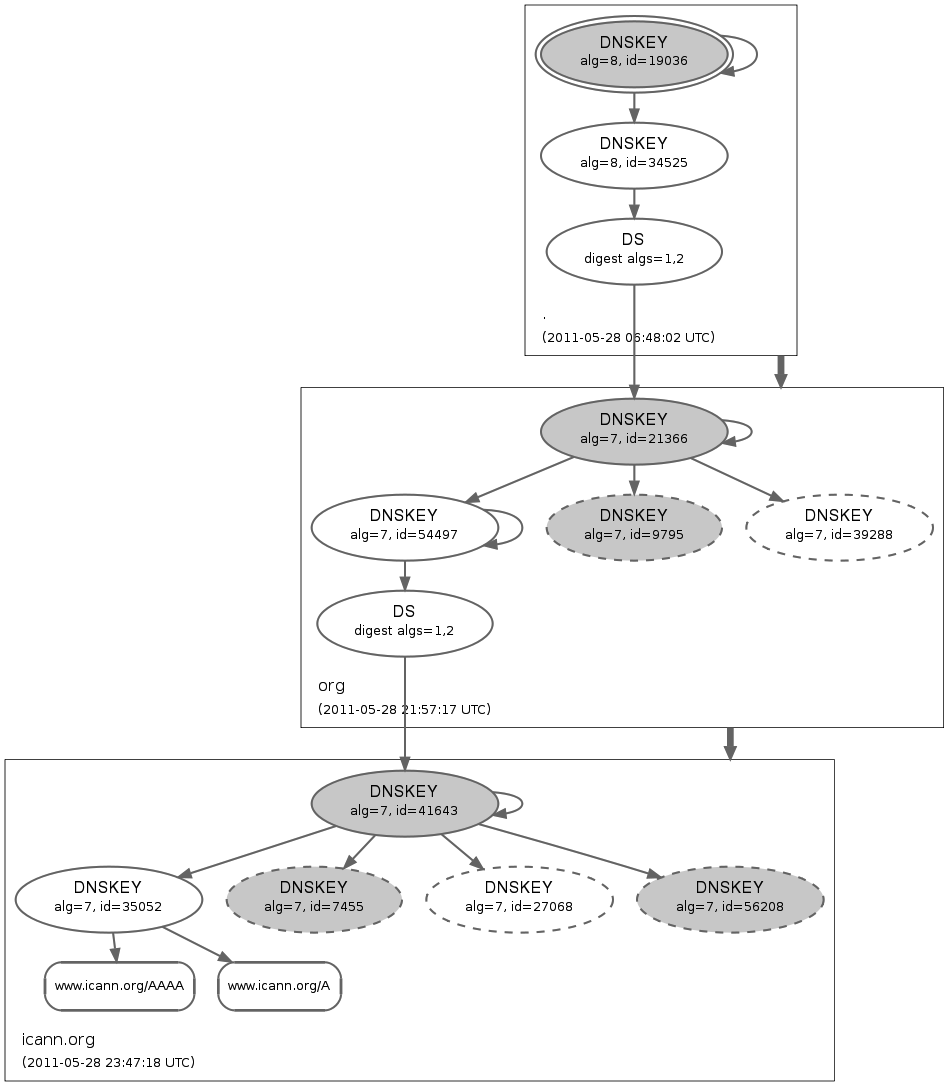
\includegraphics[width=0.7\textwidth]{imgs/18/18-43.png}
	\caption{一条可见的 DNSSEC信任链。矩形代表区域,椭圆形代表链的节点,带阴影的椭圆表示
            SEP 位置位。箭头指出了有效的 RRSIG记录或DS摘要。双圈椭圆指出了信任锚点
            18.10.3 事务认证(TSIG, TKEY, SIG(O))}
\end{figure}

\subsection{事务认证(TSIG,TKEY SIG(0))}

DNS中的一些事务,比如区域传输与动态更新,如果使用不当,可能会危害 DNS的结
构与内容。因此,它们要求某种形式的认证。如果一个解析器希望依赖于已验证的DNS解
安全:可扩展身份认证协议、IP安全协议、传輸层安全、DNS 安全,域名密钥识别邮件 649
析,但不能实现所有的 DNNSEC处理过程,那么即使是传统的DNS解析可能也需要认证。
借助交换认证,某一特定解析器与服务器之间(或在服务器之间)的交换是受保护的。需要
注意的是事务的安全并不能像 DNSSEC一样直接保护 DNS的内容。因此,DNSSEC与事务
认证是互补的,并且能够被一同部署。DNSSEC提供了数据的源认证与区域数据的完整性保
护,而事务认证客户端与服务器之间不检查交换内容正确性的特殊事务提供了完整性保护
与认证。

有两种主要的方法来认证 DNS的事务:TSIG 与 SIG(0)。TSIG 使用共享密钥而SIG(0)
使用公钥/私钥对。为了缓解部署的负担,可以使用TKEY 资源记录类型来帮助形成 TSIG
或 SIG(0)的密钥(例如,通过维护公共的DH数值)。我们将从 TSIG 开始讨论,然后研究
比较常见的交换安全机制。

\subsubsection{TSIG}
针对DNS或事务签名的密钥事务认证(TSIG)\href{https://www.rfc-editor.org/rfc/rfc2845}{[RFC2845]}使用基于共享密钥的签名为
DNS交换添加事务认证。TSIG 使用一个按需计算并且只用于保障一次事务的 TSIG 伪资源
记录。TSIG 伪资源记录中 RDATA 部分的格式如图18-44所示。
0
15 16
31
算法名称(编码为域名,长度可变)
签名时间(48位)
MAC大小(16位)
更新(16位)
MAC(长度可变)
源ID(16位)
其他长度(16位)
错误(16位)
其他数据
(长度可变,用于错误)
图18-44
TSIG 伪资源记录 RDATA 部分包含一个签名算法 ID、签名时间与时间更新参数,以及一个
消息认证码。鼓初,只使用基于MDS 的签名,但现在基于SHA-1与SHA-2 的签名已经标
准化。TSIG 端点必须在更新字段给出的秒数内完成时间同步。TSIG资源记录是由DNS消
息的附加数据部分传输的

图18-44展示了TSIG 伪资源记录的格式。这些资源记录是包含在 DNS 请求与响应的附
加数据部分发送的。\href{https://www.rfc-editor.org/rfc/rfc2845}{[RFC2845]}指出的原MAC算法是基于 HMAC-MDS 的,但更新的GS-
API(Kerberos) \href{https://www.rfc-editor.org/rfc/rfc3645}{[RFC3645]}与基于SHA-1 和SHA-256的算法已由\href{https://www.rfc-editor.org/rfc/rfc4635}{[RFC4635]}指定;当前
的列表可以在[TSIGALG]中找到。设想算法名称被编码为域名(例如,HMAC-MDS.SIG-
ALG.REG.INT),但现在大部分使用描述字符串(例如,hmac-shal,hmac-sha256)。48位的
签名时间字段是按照 UNIX 系统的时间格式(世界协调时间,从1970年1月1日开始,以
秒计时)组织的,并且给出了消息内容被签署的时间。此字段隐藏在数字签名中,被设计用
于检测并抵御重放攻击。此处使用一个绝对时间的结果是,使用TSIG 的端点必须在更新字
段指定的秒数内对时间达成一致。MAC大小字段给出了 MAC 字段中包含的MAC与其依赖
的特殊 MAC算法所需要的字节数。其他长度字段给出了其他数据字段的字节数。它们一般
只用来运送错误的消息。

为了验证 TSIG 的有效性,我们构建了一个样例区域(称 dynzone.),然后尝试进行一
次签名的动态更新。我们使用 BIND9支持的 nsupdate 程序来进行更新:
\begin{verbatim}
    Linux* nsupdate
    > zone dynzone.
    > server 127.0.0.1
    > key tsigkey.dynzone. 1234567890abcdef
    > update delete two.dynzone.
    > send
\end{verbatim}
这一系列指令形成一个使用TSIG 签名的DNS更新消息,一旦发送指令发布,TSIG就
会被发送至服务器端。图18-45显示了请求。

\begin{figure}[!htb]
    \centering
	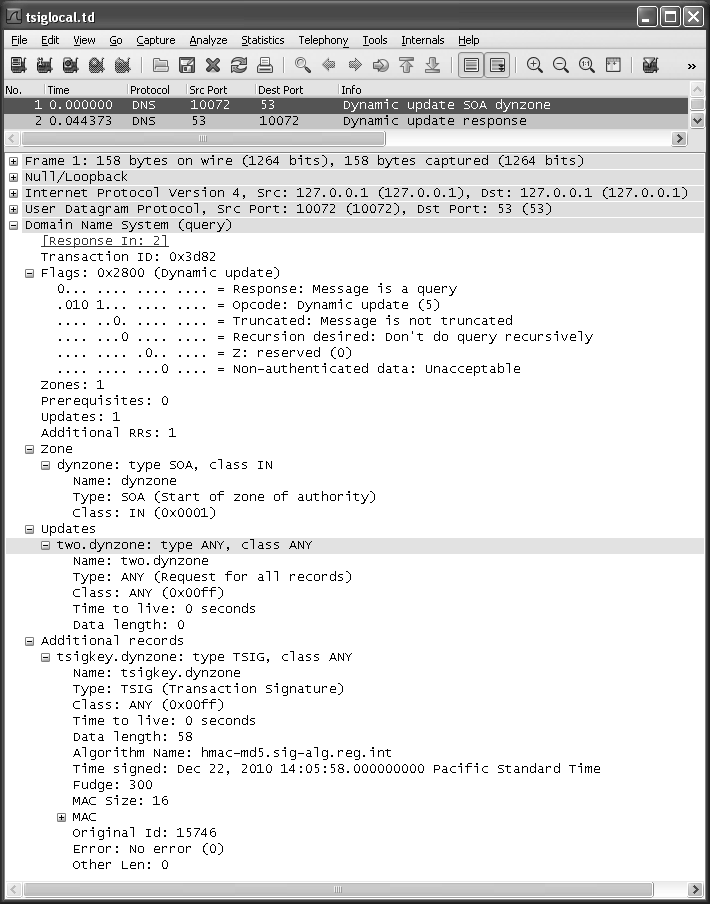
\includegraphics[width=0.7\textwidth]{imgs/18/18-45.png}
	\caption{TSIG 签署的一个 DNS动态更新请求。该请求要求删除two.dynzone.的资源记录。请求是由
            名为 tsigkey.dynzone. 的密钥签名的。签名算法HMAC-MDS,它会产生一个128位(16
            字节)的签名}
\end{figure}

在图18-45中,一个动态的DNS更新请求已由HMAC-MDS 算法签名。签名密钥的名
安全:可扩展身份认证协议、IP安全协议、传输层安全、DNS安全、域名密钥识别邮件651
称为 tsigkey. dynzone.。请求通过移除two.dynzone.这一行来更新 dynzone. 区域。签名算法
的名称次 HMAC-MDS.SIG-ALG.REG.INT,是这个软件包所支持的唯一签名算法。需要注
意的是原ID 字段(十进制15746)与交换ID 字段(0x3d82)的数值匹配。如图18-46所示,
响应确认更新已经成功。

图18-46展示了针对一个使用TSIG 签名的DNS动态更新请求做出的成功响应。标志字
段指出一个动态更新响应未包含错误。TSIG 伪资源记录又一次包含在附加信息区域中。

\begin{figure}[!htb]
    \centering
	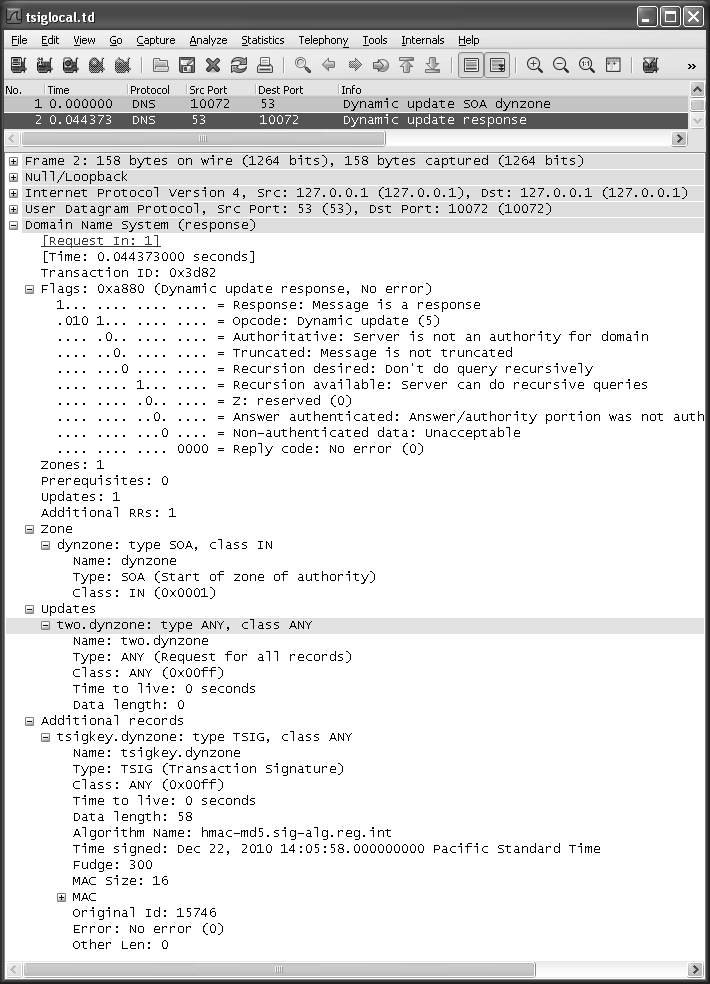
\includegraphics[width=0.7\textwidth]{imgs/18/18-46.png}
	\caption{TSIG 签署的一个 DNS动态更新响应。资源记录集 two.dynzone.已经通过动态更新成功地移除}
\end{figure}

\subsubsection{SIG(O)}
DNSSEC 的早期版本包含了与前文所讨论的现代RRSIG 资源记录相关的签名(SIG)资
源记录。然而,一种特的称为 SIG(O)的SIG 资源记录\href{https://www.rfc-editor.org/rfc/rfc2931}{[RFC2931]}没有覆盖 DNS 中静态的
记录,而是为交换动态地生成。SIG(O)的0部分指一条被签署资源记录中数据的长度。因此,
原则上 SIG(O)记录能够替代 TSIG 资源记录,并达到相同的结果。然而,它们是以不同的方
式实现的。更重要的是,SIG(0)将信任基础放置于公钥中来代替共享密钥。TSIG 被支持后
SIG(O)的流行度出现下滑,因此我们不再进一步对其进行讨论。

\subsubsection{TKEY}
TKEY元资源记录类型旨在简化 DNS 交换安全的部署,比如 TSIG 与 SIG(O)\href{https://www.rfc-editor.org/rfc/rfc2930}{[RFC2930]}。
为了完成这项工作,会动态创建TKEY 资源记录并添加到 DNS请求与响应的附加信息部分
发送出去。它们能够包含密钥或者用于形成密钥的资料,比如 DH公共数值。它可能在本地
部署中十分有用,但缺乏广泛性。
\subsection{带有 DNS64 的 DNSSEC}
第11章我们介绍了 DNS64,它能够将IPv6的DNS请求转换为IPv4 的DNS请求,并
且在IPv4 DNS中的A记录基础上合成AAAA记录。可采用一种方案,以允许只使用IPv6
的主机访问IPv4服务器与服务。DNS64通过合成 AAAA 记录进行工作。然而在 DNSSEC
中,DNS 资源记录需要被签名机构(通常为域名所有者或区域管理员)签署。这样就提出了
一个挑战:如果缺少能够生成与 DNSSEC兼容的签名的密钥,DNS64 怎样才能合成资源记
录?答案从本质上讲是否定的(参见\href{https://www.rfc-editor.org/rfc/rfc6147}{[RFC6147]}的5.5节与6.2节)。

为了在运行 DNS64时结合 DNSSEC,需要在主机端(其中 DNS64要能够实现)或
DNS64设备上执行验证函数,并且假设在存根解析器与作为递归名称服务器的 DNS64之间
有一条安全的通道。验证 DNS64 也称为vDNS64。VDNS64会解释到达请求的CD位与DO
位。如果它们都没有被置位,VDNS64 将会执行合成与验证,但是不会在(已验证的)响应
中将AD位置位。如果 DO位被置位而CD 位未被置位,VDNS64将会执行验证与合成,并
且返回一个 AD 位被置位的已验证响应(客户端大概能推测出这表示返回的资源记录是可信
的)。需要注意的是DNS64首先请求IPv4端的AAAA记录,并且在验证出这些AAAA记录
没有相同的所有者之后才合成A记录。如果 DO位与CD位均被置位,DNS64 可能会进行验
证,但不会合成。在这种情况下,客户端被认会执行验证。这种情况代表了一个潜在的问
题,如果客户端是已知安全的,但不能清楚地完成转换,那么返回的资源记录可能不能用于
IPv6 的地址域中。

\section{域名密钥识别邮件}
域名密钥识别邮件(DomainKeys Identified Mail, DKIM)\href{https://www.rfc-editor.org/rfc/rfc5585}{[RFC5585]} 意在提供一个实体
与一个域名之间的关联,从而决定哪一方发送初始消息,特别是以电子邮件的形式。它提供
了一种方法来帮助验证消息的签名者(签名者不一定是消息的发送者)。此外,它还能用于
在电子邮件分发的层面上(即,邮件代理之间)帮助治理垃圾邮件。这一工作是通过在基本
的Internet 消息格式中添加一个 DKIM 签名字段实现的[RFCS322],该字段包含了对消息头
部与消息体的数字签名。DKIM 取代了早期称为域名密钥的标准,该标准使用域名密钥签名
字段。
\subsection{DKIM签名}
为了生成一条消息的数字签名,签名域标识符(SDID)会使用RSA/SHA-1或RSA/
SHA-256算法以及相关的私钥。SDID 是来自 DNS的域名,并用于检索以TXT 资源记录存
储的公钥。一个 DKIM签名会通过Base64(比如PEM)被编码为一个消息头部字段。该签
安全:可扩展身份认证协议、IP安全协议、传输层安全、DNS 安全、域名密钥识别邮件 653
名能够签署一个明确列出的消息字段与消息体集合。例如,当接收到一封电子邮件时,邮
件传输代理会使用SDID 来实现一个 DNS查询,从而找出相关的公钥。该公钥会在之后用
于验证签名。这样就避免了请求一个 PKI 的工作。所拥有的域名是由域本身和选择器(公钥
选择器)一起构成的。例如,在域 example.com 中的选择器 key35 的公钥是一条由key35.
domainkey.example.com拥有的TXT 资源记录。

消息头部添加了DKIM 签名字段\href{https://www.rfc-editor.org/rfc/rfc6376}{[RFC6376]},而该字段又包含若干子字段(参见
[DKPARAMS]中的完整列表)。DKIM 的运行在概念上类似于 DNS 的发件人策略框架(SPF,
参见第11章),但会因为加密数字签名而变得更强大。DKIM 与 SPF 能够一起使用。
DKIM可用的域能够选择加人作者域签名实现 (Author Domain Signing Practices,
ADSP) \href{https://www.rfc-editor.org/rfc/rfc5617}{[RFC5617]}。ADSP 涉及创建一个针对某个域的机器可读的签名实现声明。这些记录
放置在使用TXT资源记录的DNS 中,所有者的名称为\verb|_adsp-_domainkey.domain.|。目前的
ADSP 记录比较简单,仅指出授权域是如何使用DKIM签名的。数值可以是未知的、全部的
或可丢弃的。这些都是接收代理对一个收到的消息可能做出操作的提示。未知的表示没有特
殊声明;全部的表示授权者签名所有的消息,但未签名的消息可能仍有价值;可丢弃的表示
未签名的消息应该考虑丢弃。可丢弃的是最严格的级别。

\subsection{例子}
为了让读者了解DKIM签名是如何出现在电子邮件中的,我们简单地抽取了一封电子邮
件的DKIM签名字段。该电子邮件来自一个大的电子邮件提供商,比如 Google 的Gmail:
\begin{verbatim}
    DKIM-Signature: v=1;a=rsa-sha256;c=relaxed/relaxed;
    d=gmail.com; s=gamma;
    h=domainkey-signature:mime-version:received:
    sender:received:date
    :X-google-sender-auth:message-id:subject:from:to:content-type;
    bh=PU2XIErWsXvhvt1W96ntPWZ2VImjVZ3VBY2T/A+WA3A=;
    b=WneQe6kpeu/BfMfa2RS1A11TVYKEIKmoORXNC
    IOJDIVoE38+fGDaj0uhNm8vXp/8kJ
    I8HqtkV4/P6/0VPMN+/5bs5dsnlhz0s/YoP
    bzx0Lt2bD67G4HPsvm6eLsaIC9rQECUSL
    MdaTBK3BgFhYo3neng3+8GxTe9I+zBCgWAVPU=
\end{verbatim}
此例指出 DKIM签名的版本号为1,而且 SHA-256摘要算法使用RSA签名。消息头与
消息体的规范算法都是“不严格的”,如“c=”字段所示。规范算法用于按照一致的形式重
写消息。当前的选项为“简单”(默认设置),它不会改变文本。“不严格的”表示能够按照常
用的方法重写输人,比如更改空格与封装较长的头部行。选择器(s=) gamma,而域(d=)
为gmail.com。稍后我们将使用这些来检索合适的公钥。用于计算签名的头字段(由“h=”
表示)包括域密钥签名(DKIM的前身)、MIME 的版本、接收发送日期、x-go0gle 发送者认证、
消息ID、主题、源以及内容类型。“bh =”子字段指出按 Base64压缩的消息体的散列值。
“b=”子字段包含了针对“h=”子字段中所列出头部的散列值而做出的RSA签名。
为了检索出公钥来验证签名,我们可以形成下面的查询:
\begin{verbatim}
    Linux8 dig gamna._domainkey.gmail.com. txt +nostats +noquestion
    i <<>> DiG 9.7.2-P3 <<>> gamma. domainkey•gmail.com.txt
    +nostats
    +noquestion
    冫冫
    global
    options: +cmd
    i; Got answer:
    i;
    ->>HEADER<<- opcode: QUERY,status: NOERROR,id: 17372
    ii flags:qr rd ra; QUERY: 1,ANSWER:1,AUTHORITY:0,ADDITIONAL:0
    :; ANSWER SECTION:
    gamma. domainkey•gmail.com. 296
    "k=rsal;t=yl;P=MIGEMAOGCS
    qGSIb3DQEBAQUAA4GNADCBiQKBgQDIhyR3oItOy2220aBrIVe9m/iME3RqOJeasANSpg2YTHTYV
    +xtp4xwE5gTjCmHQEMOsOgYuOFYiNOP0ogJ2tOMfx9zNu06rfRBDjiIU9tpx2T+NG1WZ8ghbiLo
    5By8apJavLygTLavyPSrvsxOB3YzC63T4Age2CDqZYA+OwSMWQIDAQAB"
\end{verbatim}
结果说明密钥是一个 RSA公钥。t=y条目表示域正在测试DKIM。这意味着任何 DKIM
验证的结果不应该最终影响消息的传递过程。为了查看一个ADSP的例子,我们可以执行下
面的命令:
\begin{verbatim}
    Linux& host -t txt adsp._domainkey.paypal.com.
    -adsP•_domainkey•Paypal.com
    descriptive text "dkim=discardable"
\end{verbatim}
此处我们能看到Paypal已使用最严格的DKIM签名策略,并建议丢弃 DKIM验证失败
的消息。鉴于多种的电子邮件系统与多种邮件代理重写消息的方式,使用ADSP的声明目前
是十分少见的。

\section{与安全协议相关的攻击}
有关安全协议的攻击与之前我们在其他章节中看到的协议攻击有些不同。其他章节讨论
的攻击往往会利用协议在设计与执行上的一些漏洞,从而造成危害。这些协议其实并没有真
正地进行安全设计。安全协议的攻击不仅会采用上述这些方式,而且会包含一些破坏安全所
依赖的数学基础的加密攻击。攻击能够成功地破坏较差的算法、弱的或太短的密钥,或由多
种组件构成却使得安全系统更弱的差劲组合(一个经典而有趣的例子是 VENONA 系统的密
码分析 [VENONA])。

为了理解一些针对安全协议的攻击,我们从最底层开始逐渐向上介绍。大量针对802.11
与EAP的攻击已经出现。802.11(如 WEP 和 WPATKIP)中的早期安全性已被证明是容易破
解的[TWP07][OM09]。虽然 WPA2-AES算法选择的预共享密钥(PSK)会暴露出一个巨大
的漏洞给字典攻击,但是从本质上看它是更具弹力的。

EAP 没有自己的身份认证方法,但是却继承了自己所依赖的身份认证方法的脆弱性。
此外,那些使用密钥的基于EAP 的系统,如果密钥是源于用户密码的(例如,EAP-GSS、
EAP-LEAP、EAP-SIM),也容易受到字典攻击。802.1X/EAP 容易受到包含隧道身份验证协
议的MITM 攻击(参见[ANN02])。这一问题涉及在连接双方中只有一方通过身份认证之后
如何派生出一个会话密钥。例如,如果服务器验证了一个客户端,并将这次交换作为基础通
过一个派生的会话密钥来形成一个安全的隧道,而其他验证相反方向的协议将会在隧道内运
行,那么一个扮演合法客户端的 MITM 攻击是有可能的。

已发布大量针对IPsec 的攻击,包括利用无完整性保护加密的一类攻击[PY06]。这是一
个 IPsec 文档支持但不鼓励的配置选项。从本质上看,在不被发现的前提下使用位翻转攻击
修改密文的能力,可以将加密数据报解密为那些通过可预测的方式损坏的数据报。例如,一
个正确设置了位翻转的处于隧道模式的ESP数据报可能会解码出一个数据报,该数据报通过
人为地增长 Internet 头部长度(HL)字段而使负载被当作(无效的)IP选项处理,最终产生
一条对攻击者有用的ICMP 消息。

在传输层,SSL 2.0被证明在密码套件回滚攻击中是脆弱的。在该攻击中,中间人能够
使SSL 连接的每一端都只包含一个具有弱加密能力的节点。这样就会使节点采用一个不安全
安全:可扩展身份认证协议、IP安全协议、传输层安全、DNS 安全、域名密钥识别邮件655
的密码套件,而攻击者可以利用这些密码套件。一个基于SSL/TLS的更复杂的攻击会利用
在接收端的运行顺序:解密、删除填充数据、检查 MAC。如果填充长度或消息认证码MAC
是不正确的,将会产生一条SSL 错误消息。通过观察这些错误消息的时序,就能够发起一个
Padding Oracle 攻击(参见[CHVV03])从 OpenSSH 中恢复出明文。Padding Oracle 攻击能够
分辨出明文是否用于创建一个具有有效填充量的密文。如前文所述,一个更新的攻击(TLS
1.2的)涉及中间人攻击,该攻击将一个任意长度的前缀注人一个TLS关联中,当一个合法
的客户端到达之后[RD09],该关联会被重新协商(但不会继续)。上述攻击的解决方法是将
之前的信道参数绑定到使用 TLS关联的子信道中。关于信道绑定与安全的问题在\href{https://www.rfc-editor.org/rfc/rfc5056}{[RFC5056]}
中有详细的介绍。

保障 DNS的安全已经提出很长时间,但是它的重要性通过第11 章介绍的Kaminsky缓
存位置攻击才得以重视。另一个提出较早的问题是可以利用NSEC记录发起枚举攻击,并且
还可以利用 NSEC3记录应对该攻击[BM09]。2009年年底,丹•伯恩斯坦在一次研讨会上
提出了若干关于 DNSSEC 的问题[B09]:它能够作为扩大 DoS 攻击的基础,即使在 NSEC3
中,它也会泄露区域数据,它的实现包含了可利用的错误与不能撒销的签名,加密可能会受
到密码分析,一些NS与A记录会造成漏洞。在撰写本书时,根区域只在最近才被签名,而
很少有组织会完整地采纳 DNSSEC。因此,在未来几年一些改进与修订可能会逐步实施。

18.13 总结
安全的主题是广泛而有趣的,本章只涉及了一些简单的内容。我们希望了解安全通信的
几个重要属性,通常这些属性是由机密性、可认证性、完整性以及不可否认性组合构成的。
加密是实现上述信息安全属性最重要的工具。它包含一套算法与密钥。两种重要的加密方式
是对称或“密钥”加密技术与公钥(非对称密钥)加密技术。前者拥有良好的计算性能但要
求密钥保密,而后者要求每一个个体都拥有一对密钥,并将其中之一作为公钥。公钥密码技
术能够提供认证与保障机密性的功能,并且还可以与对称密钥加密技术结合使用,从而获
得更好的性能。其他与加密技术相关的数学算法还包括用于建立对称密钥的 Diffie-Hellman
密钥协商协议,为密钥选择随机组件的伪随机函数,用于检验消息完整性的消息验证码
(MAC)。使用随机数的协议试图保证消息的时新性,它通过要求请求与响应都维护一个最近
生成的公共数值来抵御重放攻击。混淆值(在加密的意义上讲)用于干扰算法或算法的输出,
从而使字典攻击更加难以实现。

在使用公钥时,通常希望公钥能够信任的实体或组织签名认证。包含一个或多个证书颁
发机构的公钥基础设施(PKI)通常用于实现上述目标,此外信任网络模型也是一种可行的
方法。维护 PKI公钥(以及其他材料)的最常见格式是基于 PKI与证书的ITU-T X.509标准。
证书通常会被递归地签署,从而形成一棵树。整个过程以到达最高层的信任根(或信任锚点)
为结束。为了保证信任链的正确性,证书必须经过验证,从而保证证书链没有断裂,并且每
一个链节点也没有被撤销。证书的状态可以通过广泛分布的证书撤销列表(CRL)或在线协
议(比如 OCSP)来评估。整个证书验证过程也可以通过SCVP协议授权给另一方。SCVP是
专为验证证书设计的协议。

有许多用于维护证书与密钥的文件格式。DER 或CER 是一种基于 ASN.1 的二进制编
码。PEM 格式以 ASCII码形式将 DER编码表示出来,因此对应的文件易于编辑和检查。
\verb|PKCS#12|(微软PFX的前身)格式能够同时维护证书和私钥,并且它通常会被加密以保护私
钥材料。许多应用程序(比如 openssl)具有格式转换功能。

有些安全协议会针对某一个协议层,而有一些安全协议则会跨越多个协议层。虽然不会
像TCP/IP 协议那样被经常讨论,但是一些链路技术(包括它们自己的加密与认证协议)从第
2层起就开始了保障安全的工作。在TCP/IP 协议中,EAP用于建立包含多种机制的身份验
证,比如机器证书、用户证书、智能卡、密码等。EAP常用于拥有后台认证或AAA服务器
的企业设置。EAP 还可以用于其他协议的认证,比如 IPsec。

IPsec 是一个提供第3层安全的协议集合,其中包括IKE、AH以及ESP。IKE建立并
管理双方之间的安全关联。安全关联涉及认证(AH)或加密(ESP),并且能够运行于传输
或隧道模式。在传输模式中,会修改IP 头部以进行认证或加密,而在隧道模式中,IP数
据报会被完全放置在一个新的IP 数据报中。ESP 是IPsec 最流行的协议。所有的IPsec 协
议能够使用不同的算法与参数(加密套件)进行加密、完整性保护、DH密钥协商以及身份
认证。

沿协议栈向上查看,传输层安全(当前版本为 TLS 1.2)保护了两个应用程序之间的信
息。它拥有自己的内部分层,包含一个记录层协议和三个信息交换协议:密码更改协议、警
告协议、握手协议。此外,记录协议支持应用数据。记录层负责根据握手协议提供的参数
加密数据并保障它们的完整性。密码更改协议用于将之前设定的挂起协议状态更改为活动协
议状态。警告协议会指出错误或连接问题。与TCP/IP一起使用的TLS 是使用最广泛的安全
协议,并且它还支持加密的web 浏览器连接(HTTPS)。TLS的一个变种称为DTLS,它将
TLS应用于数据报协议,比如 UDP与DCCP。

为了更好地保护主机名与 Web 的安全,DNSSEC致力于为DNS提供安全保障。2010
年7月15日,Internet 的签名根区域投人运行,从而满足了全球部署的一个先决条件。
DNSSEC借助DNS中的几个新资源记录工作,其中包括 DNSKEY、DS、NSEC/NSEC3/
NSEC3PARAM以及 RRSIG。前两个资源记录用于指出并维护负责签名某一区域结构与内容
的公钥。NSEC或NSEC3/NSEC3PARAM记录有助于提供一个规范有序的名称和域名的类型
列表。RRSIG 记录维护了其他记录中的签名与签署区域,区域中所有的权威资源记录必须有
相关的RRSIG 资源记录。一旦被设置,DNS 查询的安全性会被一个 DNS验证解析器或请求
一个信任锚点的名称服务器检查。这样的系统通过检查来保证数字签名与 DNS提供的公钥
相匹配。当发现一些记录不一致时,它允许生成错误,同时,它也能够抵御那种攻击者伪装
成合法主机的域名劫持攻击。在一些情况下,DNS交换也会受到安全保护。TSIG 与 SIG(O)
协议提供了一种信道认证形式,但只适用于DNS交换的范围。这些协议用于诸如 DNS动态
更新和区域转移之类的交换。

安全协议的攻击不仅包含了那些常见的利用实现漏洞和不安全的设计的攻击,还包含
了数学危害以及用于发现秘密信息的“侧信道”攻击(例如,密钥的比特位)。多年来,在
用于安全通信的密码技术中,满足灵活性的需求已经成为明确的共识,因此我们讨论的绝
大多数协议都提供了加密套件。这些加密套件会随着计算能力的提高与额外经验的获取而
不断发展。许多看似安全的协议,即便受到专家的广泛审查,也已经成为一帮精力充沛的
分析者的“猎物”。这些分析者会寻找可以利用的错误,尤其是那些使中间人或其他主动
攻击成为可能的错误。在设计新的安全协议及按照安全的方式运行现有协议时,需要格外
小心。


18.14 参考文献

\begin{verbatim}
    [802.1X-2010]'TEEE Standard for Port-Based Network Access Control," IEEE Std
    802.1X-2010, Feb.2010.
    [AKNTO4] Y. Amir, Y. Kim, C. Nita-Rotaru, and G. Tsudik, "On the Performance
    of Group Key Agreement Protocols.” ACM Transactions on Information and System
    Security, 7(3), Aug. 2004.
    IANNO2] N.Asokan, V. Niemi, and K. Nyberg, "Man-in-the-Middle in Tunnelec
    Authentication Protocols (Extended Abstract)" Proc. 11th Security Protocols Work.
    shop/LNCS 3364 (Springer, 2003).
    [B06] M. Bellare, "New Proofs for NMAC and HMAC: Security without
    Collision-Resistance" (preliminary version in CRYPTO 06), June 2006.
    [B09] D. Bernstein, "Breaking DNSSEC." keynote talk at Workshop on Offensive
    Technologies (WOOT), Aug. 2009.
    [BCK96] M. Bellare, R. Canetti, and H. Krawczyk, "Keying Hash Functions for
    Message Authentication" (abridged version in CRYPTO 96/LNCS 1109), June
    1996.
    [BM09]J. Bau and J. Mitchell, "A Security Evaluation of DNSSEC with NSEC3"
    Network and Distributed System Security Symposium (NDSS), Feb.-Mar. 2010.
    [BOPSW09] R. Biddle et al., "Browser Interfaces and Extended Validation SSL
    Certificates: An Empirical Study" Proc. ACM Cloud Security Workshop, Nov. 2009.
    [CABF09] CA/Browser Forum, "Guidelines for the Issuance and Management
    of Extended Validation Certificates (v1.2),” 2009,http://www.cabforum.org/
    Guidelines_V1_2.pdf
    ICHP] National Institute of Standards and Technology, Cryptographic Hash
    Project, Computer Security Division—Computer Security Resource Center,
    http://csrc.nist.gov/groups/ST/hash
    [CHVV03] B. Canvel, A. Hiltgen, S. Vaudenay, and M. Vuagnoux, "Password
    Interception in a SSL/TLS Channel/" CRYPTO 2003/LNCS 2729.
    [DH76] W. Diffie and M. Hellman,"New Directions in Cryptography."IEEE
    Transactions on Information Theory, IT-22, Nov. 1976.
    IDKPARAMS] http://www.iana.org/assignments/dkim-parameters
    [DNSSECALG] http://www.iana.org/assignments/dns-sec-alg-numbers
    [DOW92] W. Diffie, P. Oorschot, and M. Wiener, "Authentication and uthenti-
    cated Key Exchanges"' Designs, Codes and Cryptography, 2,June 1992.
    [DSRRTYPES] http://www.iana.org/assignments/ds-rr-types
    [FIPS186-3] National Institute for Standards and Technology, "Digital Signature
    Standard (DSS)" FIPS PUB 186-3, June 2009.
    [FIPS197] National Institute for Standards and Technology, "Advanced Encryp-
    tion Standard (AES)" FIPS PUB 197, Nov. 2001.
    TFIPS198] National Institute for Standards and Technology, "The Keyed-Hash
    Message Authentication Code (HMAC)" FIPS PUB 198, Mar. 2002.
    【FIPS800-38B] National Institute for Standards and Technology, "Recommenda-
    tion for Block Cipher Modes of Operation: The CMAC Mode for Authentication,"
    NIST Special Publication 800-38B, May 2005.
    [GGM86] 0. Goldreich, S. Goldwasser, and S. Micali, "How to Construct Random
    Functions," Journal of the ACM, 33(4), Oct. 1986.
    658
    第18章
    [IDDCIN] S. Weiler and D. Blacka, "Clarifications and Implementation Notes for
    DNSSECbis" Internet draft-ietf-dnsext-dnssec-bis-updates, work in progress,
    July 2011.
    [IDDS2] B. Dickson, "DNSSEC Delegation Signature with Canonical Signer
    Name" Internet draft-dickson-dnsext-ds2 (expired), work in progress, Nov. 2010.
    [IDDTLS] E. Rescorla and N. Modadugu, "Datagram Transport Layer Security
    Version 1.2" Internet draft-ietf-tls-rfc4347-bis, work in progress, July 2011.
    [IEAP] http://www.iana.org/assignments/eap-numbers
    [IK03] T. Iwata and K. Kurosawa, "OMAC: One-Key CBC MAC," Proc. Fast Soft-
    ware Encryption, Mar. 2003.
    [IKEPARAMS] http://www.iana.org/assignments/ikev2-parameters
    IIPANA]http://www.iana.org/assignments/pana-parameters
    [ITUOID] http://www.itu.int/ITU-T/asn1
    [IWESPJ http://www.iana.org/assignments/wesp-flags
    [K87] N. Koblitz, "Elliptic Curve Cryptosystems;" Mathematics of Computation, 48,
    1987.
    [LO1] C. Landwehr, "Computer Security" Springer-Verlag Online, July 2001.
    [M85| V.Miller, "Uses of Elliptic Curves in Cryptography." Advances in Cryptol-
    0gY: CRYPTO '85, Lecture Notes in Computer Science, Volume 218 (Springer-
    Verlag, 1986).
    [MSK09] S.McClure, J. Scambray, and G. Kurtz, Hacking Exposed, Sixth Edition
    (McGraw-Hill, 2009).
    [MW99】 U. Maurer and S. Wolf, "The Relationship between Breaking the Diffie-
    Hellman Protocol and Computing Discrete Logarithms," Siam Journal on Comput-
    ing, 28(5), 1999.
    [NAZ00] Network Associates and P. Zimmermann, Introduction to Cryptogta-
    phy, Part of PGP 7.0 Documentation, available from http://www.pgpi.org/doc/
    guide/7.0/en
    [NIST800-38B] National Institute for Standards and Technology, "Recommenda-
    tion for Block Cipher Modes of Operation: Galois/Counter Mode (GCM) and
    GMAC" NIST Special Publication 800-38D, Nov. 2005.
    INSEC3PARAMS] http://www.iana.org/assignments/dnssec-nsec3-parameters
    [OM09] T. Ohigashi and M. Morii, "A Practical Message Falsification Attack on
    WPA," Joint Workshop on Information Security, Aug. 2009.
    [PY06] K. Paterson and A. Yau, "Cryptography in Theory and Practice: The Case
    of Encryption in IPsec," EUROCRYPT 2006/LNCS 4004.
    [RD09] M. Ray and S. Dispensa, "Renegotiating TLS" PhoneFactor Technical
    Report, Nov. 2009.
    [RSA78] R. Rivest, A. Shamir, and L. Adleman, "A Method for Obtaining Digital
    Signatures and Public Key Cryptosystems," Communications of the ACM, 21(2),
    Feb. 1978.
    [TLD-REPORT] http://stats.research.icann.org/dns/tld_report
    [TLSEXT] http://www.iana.org/assignments/tls-extensiontype-values
    [TLSPARAMS] http://www.iana.org/assignments/tls-parameters
    [TNMOC]The National Museum of Computing, http://www.tnmoc.org
    [TSIGALG] http://www.iana.org/assignments/tsig-algorithm-names
    [TWPO7] E. Tews, R. Weinmann, and A. Pyshkin, "Breaking 104 Bit WEP in Less
    than 60 Seconds" Proc.8th International Workshop on Information Security Applica-
    tions (Springer, 2007).
    IVENONA] R. L. Benson, National Security Agency Center for Cryptologic Flis-
    tory, "The VENONA Story." http://www.nsa.gov/public_info/declass/venona
    安全:可扩展身份认证协议、IP安全协议、传输层安全、DNS 安全、域名密钥识别邮件665
    [VK83] V. Voydock and S. Kent, "Security Mechanisms in High-Level Network
    Protocols/" ACM Computing Surveys, 15, June 1983.
    [WY05] X. Wang and H. Yu, "How to Break MD5 and Other Hash Functions,"
    EUROCRYPT, May 2005.
    [X9.62-2005] American National Standards Institute, "Public Key Cryptography
    for the Financial Services Industry: The Elliptic Curve Digital Signature Stan-
    dard (ECDSA)" ANSI X9.62, 2005.
    [Z97] Y. Zheng, "Digital Signcryption or How to Achieve Cost(Signature &
    Encryption) << Cost(Signature) + Cost(Encryption)" Proc. CRYPTO, Lecture
    Notes in Computer Science, Volume 1294 (Springer-Verlag, 1997).
\end{verbatim}
缩略语
3GPP
3GPP2
6rd
6to4
A
AAA
AAAA
ABC
133
AC
ACCM
ACD
ACFC
ACK
ACL
ADSP
AEAD
AES
AF
AFTR
AH
AIA
AIAD
AIMD
ALG
A-MPDU
第三代合作伙伴计划(针对GSM、W-CDMA、LTE 等的蜂窝标准制定组织)
第三代合作伙伴计划2(针对CDMA2000、EV-DO 等的蜂窝标准制定组织)
IPv6 快速部署(一种通过IPv4 网络传输 IPv6 流量的过渡机制,它与6to4
方法类似,但在单播地址分配的基础上对IPv6 前缀进行分配)
IPv6 到IPv4(在IPv4 隧道中传输 IPv6流量,目前已遇到一些运营挑战)
地址(IPv4)(在DNS资源记录中,描述一个 IPv4地址)
认证、授权和计费(与某些访问协议相关的管理功能,例如 RADIUS与
Diameter 协议)
地址(IPv6)(在 DNS资源记录中,描述一个 IPv6地址)
适当字节计数(在TCP 拥塞控制中,一种统计确认后的字节数的方法,用
于代替执行CWND计算时的常数因子;它可以减轻由ACK 延迟而引发的
窗口缓慢增长问题)
属性证书(一种认证类型,用于包含某些属性,例如授权的证书。该证书与
PKC的不同之处在于它不包含公钥)
异步控制字符映射(在PPP 中,指出需要被转义的字节,以避免不期望的
影响)
自动冲突检测(检测与避免IP 地址分配冲突的程序)
地址和控制字段压缩(在PPP中,压缩地址和控制字段以减少开销)
确认(一种表明数据已经成功到达接收端的提示,适用于协议栈的多个
层次)
访问控制列表(一种流量过滤规则列表,例如是否允许通过防火墙)
作者域签名实现(一种关于 DKIM 如何使用或部署于特定域中的策略状态)
认证加密相关的数据(对输人的一部分进行加密和认证,对另一部分只进行
认证的算法)
高级加密标准(美国目前使用的新一代加密标准)
保证转发(一种提供流量类优先级与类间优先次序的 PHB)
地址族转换路由器(在DS-Lite 中,一种将少量IPv4地址分享给多个用户的
SPNAT)
认证头部(可选的IPsec协议对IP 流量所提供的认证服务,包括头部信息,
但它与 NAT不兼容)
权威信息访问(X.509证书的一种扩展,它在验证一个证书时指明可用的
资源)
和式增加,和式减少(TCP 中用于限制CWND的方法,在拥塞度较低时增
加该数值,在拥塞度较高时减少该数值;但它并不是标准的TCP 算法)
和式增加,积式减少(TCP 中用于限制CWND的方法,在拥塞度较低时增
加该数值,在拥塞度较高时将该数值乘以小于1的分数)
应用层网关(一种在应用层完成协议转换任务的代理,通常是软件)
聚合的MPDU(包含多个 MPDU 的帧,是【EEE 802.11n 协议的一部分)
